%%% Hlavní soubor. Zde se definují základní parametry a odkazuje se na ostatní části. %%%

%% Verze pro jednostranný tisk:
% Okraje: levý 40mm, pravý 25mm, horní a dolní 25mm
% (ale pozor, LaTeX si sám přidává 1in)
\documentclass[12pt,a4paper]{report}
\setlength\textwidth{145mm}
\setlength\textheight{247mm}
\setlength\oddsidemargin{15mm}
\setlength\evensidemargin{15mm}
\setlength\topmargin{0mm}
\setlength\headsep{0mm}
\setlength\headheight{0mm}
% \openright zařídí, aby následující text začínal na pravé straně knihy
\let\openright=\clearpage

%% Pokud tiskneme oboustranně:
% \documentclass[12pt,a4paper,twoside,openright]{report}
% \setlength\textwidth{145mm}
% \setlength\textheight{247mm}
% \setlength\oddsidemargin{14.2mm}
% \setlength\evensidemargin{0mm}
% \setlength\topmargin{0mm}
% \setlength\headsep{0mm}
% \setlength\headheight{0mm}
% \let\openright=\cleardoublepage

%% Vytváříme PDF/A-2u
\usepackage[a-2u]{pdfx}

%% Přepneme na českou sazbu a fonty Latin Modern
\usepackage[czech]{babel}
\usepackage{lmodern}
\usepackage[T1]{fontenc}
\usepackage{textcomp}

%% Použité kódování znaků: obvykle latin2, cp1250 nebo utf8:
\usepackage[utf8]{inputenc}

%%% Další užitečné balíčky (jsou součástí běžných distribucí LaTeXu)
\usepackage{amsmath}        % rozšíření pro sazbu matematiky
\usepackage{amsfonts}       % matematické fonty
\usepackage{amsthm}         % sazba vět, definic apod.
\usepackage{bbding}         % balíček s nejrůznějšími symboly
			    % (čtverečky, hvězdičky, tužtičky, nůžtičky, ...)
\usepackage{bm}             % tučné symboly (příkaz \bm)
\usepackage{graphicx}       % vkládání obrázků
\usepackage{fancyvrb}       % vylepšené prostředí pro strojové písmo
\usepackage{indentfirst}    % zavede odsazení 1. odstavce kapitoly
\usepackage{natbib}         % zajištuje možnost odkazovat na literaturu
			    % stylem AUTOR (ROK), resp. AUTOR [ČÍSLO]
\usepackage[nottoc]{tocbibind} % zajistí přidání seznamu literatury,
                            % obrázků a tabulek do obsahu
\usepackage{icomma}         % inteligetní čárka v matematickém módu
\usepackage{dcolumn}        % lepší zarovnání sloupců v tabulkách
\usepackage{booktabs}       % lepší vodorovné linky v tabulkách
\usepackage{paralist}       % lepší enumerate a itemize
\usepackage[usenames]{xcolor}  % barevná sazba

%%% Údaje o práci

% Název práce v jazyce práce (přesně podle zadání)
\def\NazevPrace{Tau Ceti f 2 – budovatelská počítačová hra se strategickými prvky}

% Název práce v angličtině
\def\NazevPraceEN{Tau Ceti f 2 – A Creative Computer Game with Strategic Elements}

% Jméno autora
\def\AutorPrace{Pavel Halbich}

% Rok odevzdání
\def\RokOdevzdani{2017}

% Název katedry nebo ústavu, kde byla práce oficiálně zadána
% (dle Organizační struktury MFF UK, případně plný název pracoviště mimo MFF)
\def\Katedra{Katedra distribuovaných a spolehlivých systémů}
\def\KatedraEN{Department of Distributed and Dependable Systems}

% Jedná se o katedru (department) nebo o ústav (institute)?
\def\TypPracoviste{Katedra}
\def\TypPracovisteEN{Department}

% Vedoucí práce: Jméno a příjmení s~tituly
\def\Vedouci{Mgr. Pavel Ježek, Ph.D.}

% Pracoviště vedoucího (opět dle Organizační struktury MFF)
\def\KatedraVedouciho{Katedra distribuovaných a spolehlivých systémů}
\def\KatedraVedoucihoEN{Department of Distributed and Dependable Systems}

% Studijní program a obor
\def\StudijniProgram{Informatika }
\def\StudijniObor{Programování a softwarové systémy}

% Nepovinné poděkování (vedoucímu práce, konzultantovi, tomu, kdo
% zapůjčil software, literaturu apod.)
\def\Podekovani{%
Děkuji mému vedoucímu Pavlu Ježkovi za pomoc s touto prací, mým rodičům za podporu a pevné nervy, mé přítelkyni Veronice taktéž za podporu a pomoc s 2D grafikou a Jiřímu Kurčíkovi za laskavé poskytnutí práv na použití jeho hudební tvorby v mé hře. 
}

% Abstrakt (doporučený rozsah cca 80-200 slov; nejedná se o zadání práce)
\def\Abstrakt{%
Abstrakt.
}
\def\AbstraktEN{%
Abstract.
}

% 3 až 5 klíčových slov (doporučeno), každé uzavřeno ve složených závorkách
\def\KlicovaSlova{%
{klíčová} {slova}
}
\def\KlicovaSlovaEN{%
{key} {words}
}

%% Balíček hyperref, kterým jdou vyrábět klikací odkazy v PDF,
%% ale hlavně ho používáme k uložení metadat do PDF (včetně obsahu).
%% Většinu nastavítek přednastaví balíček pdfx.
\hypersetup{unicode}
\hypersetup{breaklinks=true}

%% Definice různých užitečných maker (viz popis uvnitř souboru)
%%% Tento soubor obsahuje definice různých užitečných maker a prostředí %%%
%%% Další makra připisujte sem, ať nepřekáží v ostatních souborech.     %%%

%%% Drobné úpravy stylu

% Tato makra přesvědčují mírně ošklivým trikem LaTeX, aby hlavičky kapitol
% sázel příčetněji a nevynechával nad nimi spoustu místa. Směle ignorujte.
\makeatletter
\def\@makechapterhead#1{
  {\parindent \z@ \raggedright \normalfont
   \Huge\bfseries \thechapter. #1
   \par\nobreak
   \vskip 20\p@
}}
\def\@makeschapterhead#1{
  {\parindent \z@ \raggedright \normalfont
   \Huge\bfseries #1
   \par\nobreak
   \vskip 20\p@
}}
\makeatother

% Toto makro definuje kapitolu, která není očíslovaná, ale je uvedena v obsahu.
\def\chapwithtoc#1{
\chapter*{#1}
\addcontentsline{toc}{chapter}{#1}
}

% Trochu volnější nastavení dělení slov, než je default.
\lefthyphenmin=2
\righthyphenmin=2

% Zapne černé "slimáky" na koncích řádků, které přetekly, abychom si
% jich lépe všimli.
\overfullrule=1mm

%%% Makra pro definice, věty, tvrzení, příklady, ... (vyžaduje baliček amsthm)

\theoremstyle{plain}
\newtheorem{veta}{Věta}
\newtheorem{lemma}[veta]{Lemma}
\newtheorem{tvrz}[veta]{Tvrzení}

\theoremstyle{plain}
\newtheorem{definice}{Definice}

\theoremstyle{remark}
\newtheorem*{dusl}{Důsledek}
\newtheorem*{pozn}{Poznámka}
\newtheorem*{prikl}{Příklad}

%%% Prostředí pro důkazy

\newenvironment{dukaz}{
  \par\medskip\noindent
  \textit{Důkaz}.
}{
\newline
\rightline{$\square$}  % nebo \SquareCastShadowBottomRight z balíčku bbding
}

%%% Prostředí pro sazbu kódu, případně vstupu/výstupu počítačových
%%% programů. (Vyžaduje balíček fancyvrb -- fancy verbatim.)

\DefineVerbatimEnvironment{code}{Verbatim}{fontsize=\small, frame=single}

%%% Prostor reálných, resp. přirozených čísel
\newcommand{\R}{\mathbb{R}}
\newcommand{\N}{\mathbb{N}}

%%% Užitečné operátory pro statistiku a pravděpodobnost
\DeclareMathOperator{\pr}{\textsf{P}}
\DeclareMathOperator{\E}{\textsf{E}\,}
\DeclareMathOperator{\var}{\textrm{var}}
\DeclareMathOperator{\sd}{\textrm{sd}}

%%% Příkaz pro transpozici vektoru/matice
\newcommand{\T}[1]{#1^\top}

%%% Vychytávky pro matematiku
\newcommand{\goto}{\rightarrow}
\newcommand{\gotop}{\stackrel{P}{\longrightarrow}}
\newcommand{\maon}[1]{o(n^{#1})}
\newcommand{\abs}[1]{\left|{#1}\right|}
\newcommand{\dint}{\int_0^\tau\!\!\int_0^\tau}
\newcommand{\isqr}[1]{\frac{1}{\sqrt{#1}}}

%%% Vychytávky pro tabulky
\newcommand{\pulrad}[1]{\raisebox{1.5ex}[0pt]{#1}}
\newcommand{\mc}[1]{\multicolumn{1}{c}{#1}}


%% Titulní strana a různé povinné informační strany
\begin{document}
%%% Titulní strana práce a další povinné informační strany

%%% Titulní strana práce

\pagestyle{empty}
\hypersetup{pageanchor=false}

\begin{center}

\centerline{\mbox{
\includegraphics[width=166mm]{../img/logo-cs.pdf}}}

\vspace{-8mm}
\vfill

{\bf\Large BAKALÁŘSKÁ PRÁCE}

\vfill

{\LARGE\AutorPrace}

\vspace{15mm}

{\LARGE\bfseries\NazevPrace}

\vfill

\Katedra

\vfill

\begin{tabular}{rl}

Vedoucí bakalářské práce: & \Vedouci \\
\noalign{\vspace{2mm}}
Studijní program: & \StudijniProgram \\
\noalign{\vspace{2mm}}
Studijní obor: & \StudijniObor \\
\end{tabular}

\vfill

% Zde doplňte rok
Praha \RokOdevzdani

\end{center}

\newpage

%%% Následuje vevázaný list -- kopie podepsaného "Zadání bakalářské práce".
%%% Toto zadání NENÍ součástí elektronické verze práce, nescanovat.

%%% Strana s čestným prohlášením k bakalářské práci

\openright
\hypersetup{pageanchor=true}
\pagestyle{plain}
\pagenumbering{roman}
\vglue 0pt plus 1fill

\noindent
Prohlašuji, že jsem tuto bakalářskou práci vypracoval(a) samostatně a výhradně
s~použitím citovaných pramenů, literatury a dalších odborných zdrojů.

\medskip\noindent
Beru na~vědomí, že se na moji práci vztahují práva a povinnosti vyplývající
ze zákona č. 121/2000 Sb., autorského zákona v~platném znění, zejména skutečnost,
že Univerzita Karlova má právo na~uzavření licenční smlouvy o~užití této
práce jako školního díla podle §60 odst. 1 autorského zákona.

\vspace{10mm}

\hbox{\hbox to 0.5\hsize{%
V ........ dne ............
\hss}\hbox to 0.5\hsize{%
Podpis autora
\hss}}

\vspace{20mm}
\newpage

%%% Poděkování

\openright

\noindent
\Podekovani

\newpage

%%% Povinná informační strana bakalářské práce

\openright

\vbox to 0.5\vsize{
\setlength\parindent{0mm}
\setlength\parskip{5mm}

Název práce:
\NazevPrace

Autor:
\AutorPrace

\TypPracoviste:
\Katedra

Vedoucí bakalářské práce:
\Vedouci, \KatedraVedouciho

Abstrakt:
\Abstrakt

Klíčová slova:
\KlicovaSlova

\vss}\break\vbox to 0.49\vsize{
\setlength\parindent{0mm}
\setlength\parskip{5mm}

Title:
\NazevPraceEN

Author:
\AutorPrace

\TypPracovisteEN:
\KatedraEN

Supervisor:
\Vedouci, \KatedraVedoucihoEN

Abstract:
\AbstraktEN

Keywords:
\KlicovaSlovaEN

\vss}

\newpage

\openright
\pagestyle{plain}
\pagenumbering{arabic}
\setcounter{page}{1}


%%% Strana s automaticky generovaným obsahem bakalářské práce

\tableofcontents

%%% Jednotlivé kapitoly práce jsou pro přehlednost uloženy v samostatných souborech
%!TEX root = ../../prace.tex

\chapter{Úvod}

V době vzniku této práce jsou velice populární hry s~otevřeným světem. Lákají hráče na obsáhlost světa a~možnost nelineárního řešení problémů a~herních úkolů. Her s~otevřeným světem najdeme nepřeberné množství v~různých herních žánrech. My se zaměříme na podmnožinu her, které kromě otevřeného světa nabízí také možnosti budování struktur a~vyžadují od hráče netriviální styl hraní, který mu umožňuje ve hře přežít. V herním průmyslu se tyto hry často označují jako \textit{sanboxové}, \textit{s budováním}, \textit{s průzkumem prostředí}, \textit{o přežití}. Autor této práce má tento typ her v~oblibě a~rád by touto prací představil svoji vizi dalšího možného rozvoje her tohoto žánru. Cílem práce by měla být implementace nového herního principu stavění, které současné herní tituly nenabízí.

\section{Charakteristika her}
V práci se budeme zabývat několika různými hrami, které však mají několik společných vlastností. Jedním ze základních konceptů je využívání herních bloků. Dalším význačným prvkem je způsob integrace herních bloků do herního prostření. Některé hry jsou celé tvořeny bloky, jiné se snaží dosáhnout vyššího stupně realismu ve hře a~bloky využívají pouze pro konstrukci různých herních objektů. Důležitým tématem této práce tedy bude rozbor systému bloků a~práce s~nimi a~popis hráčských problémů způsobených danými koncepty. V další části práce pak navrhneme a~implementujeme vlastní řešení.




\subsection{Hry kompletně blokové}
Začněme hrami, které využívají bloků jako základního elementu celé hry. Bloky zde tvoří doslova celý svět. Mezi nejpopulárnější a~širokou veřejností nejznámější bychom měli zařadit hru \MC{}. Na obrázku z této hry \ref{fig:intro_mc} si můžeme všimnout několika zásadních faktů. Vidíme zde kostičkované listí stromů (1) či hrad na skále (2), který byl postaven z~kostiček. Taktéž slunce, měsíc a~mraky (3) jsou stylizovány do kostiček. Výrazně je kostičkovaný styl vidět na nehratelných postavách (\textit{non-playable character} -- \NPC{}) -- na obrázku ovce (4), krávy a~prasata. Stejným způsobem je pak zpracován i~hráčův charakter (5), tedy postava, kterou hráč přímo ovládá.

TODO zmínit crafting, stavěnbí

\begin{figure}[!ht]\centering
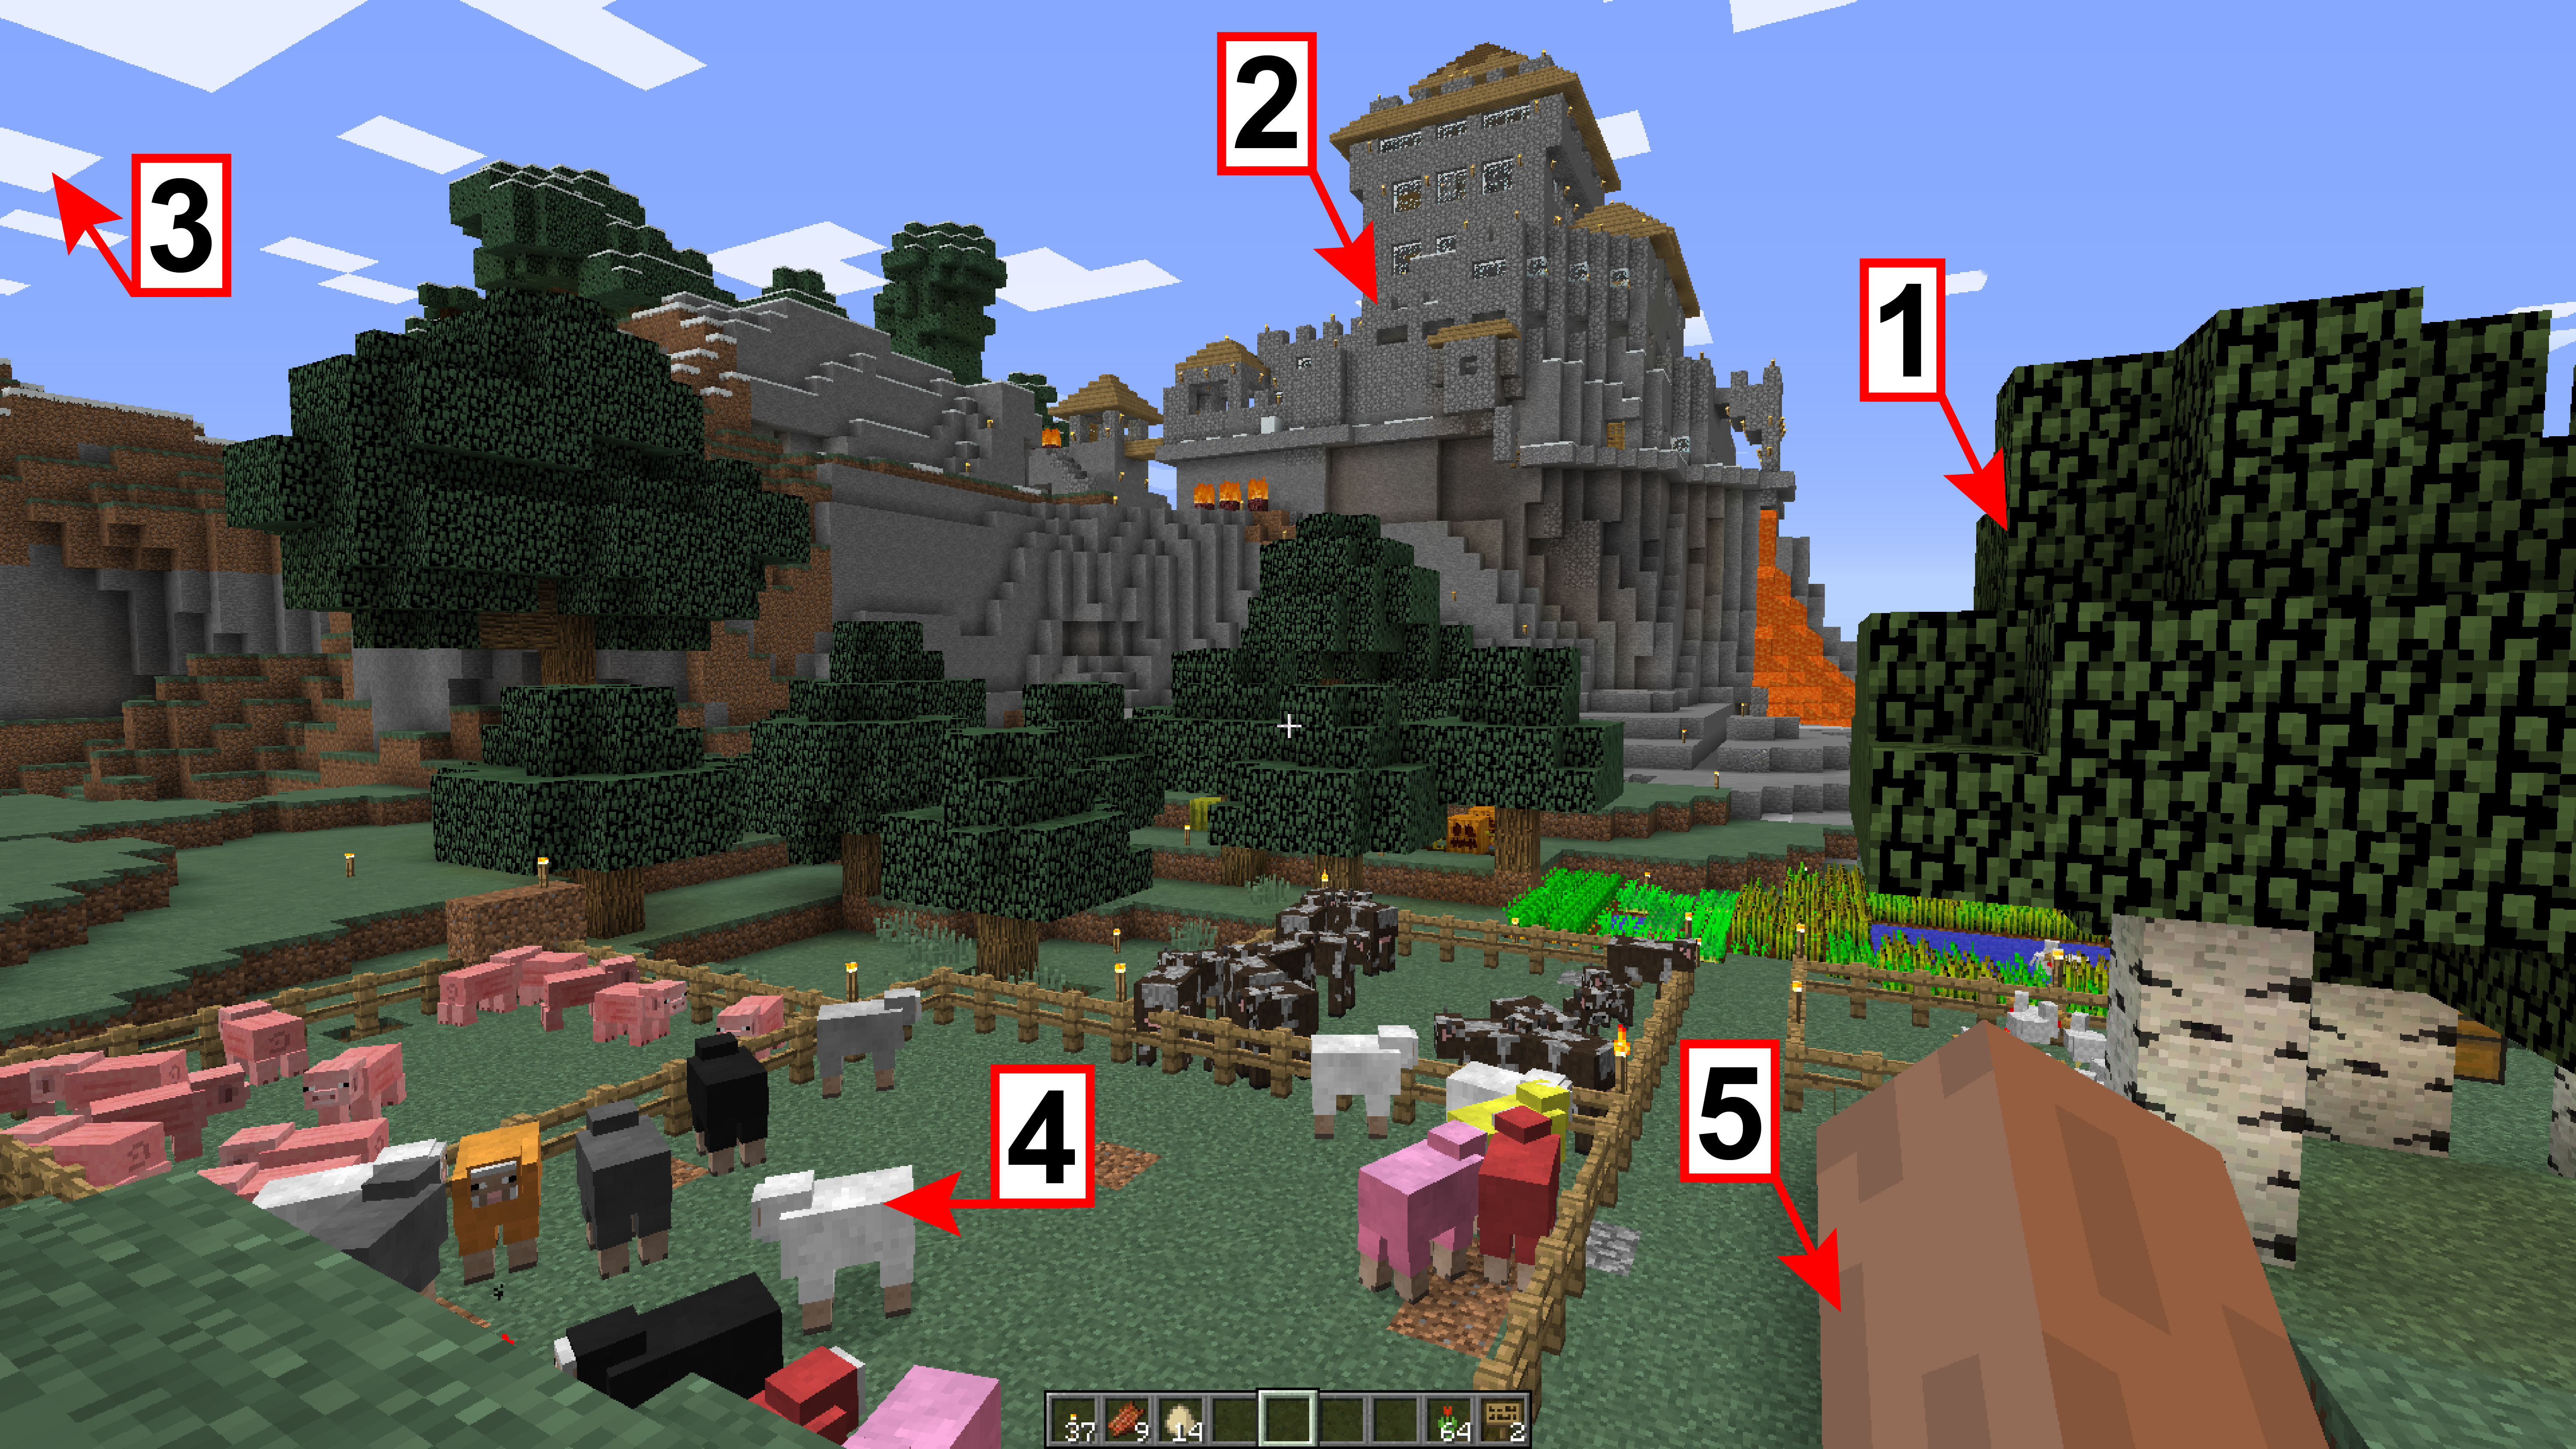
\includegraphics[ width=140mm]{../img/intro/mc}

\caption{Hra Minecraft - hrad na skále}
\label{fig:intro_mc}

\end{figure}

\FloatBarrier

Mezi dalšími hrami bychom mohli zmínit například \TE{}. Ta je o~něco mladší než \MC{}, ale je častým zdrojem diskusí, zda je lepší new \MC{}, nebo ne. Pravdou je, že obě hry mají svůj svět kompletně složený z~kostek (\TE{} je však 2D hra), ale každá si klade trochu jiné cíle. \TE{} je více orientovaná na příběh, obsahuje více \NPC{} i~bossů. Boss je v~herní terminologii významný nepřítel, obvykle je silnější než ostatní protivníci a~velmi často bývá v~závěrečných částech hry. Duel s~bossem pak obvykle od hráče vyžaduje zjištění jeho silných a~slabých stránek a~schémat jeho útoků \citep{intro_boss}. \MC{} je pak orientován spíše na stavění. (Porovnání Minecraft vs Terraria (facts) \citep{mc_te_comparsion} na Minecraftovém fóru.)


\subsection{Hry s~prvky realismu}

Mezi hry s~prvky realismu bychom mohli zařadit třeba hry \SE{} či \ME{}, využívají kombinaci herních bloků s~\textit{voxelovou} reprezentací světa. Obě hry jsou implementovány v~proprietárním enginu společnosti Keen Software House nazvaném \textit{VRAGE}\texttrademark{}. Voxelový terén je pak v~enginu za běhu hry procedurálně generován do polygonální reprezentace, kterou pak grafická karta standardním způsobem vykreslí na obrazovce (oficiální popis vlastností enginu \citep{vrage}). Během tohoto procedurálního vytváření je na třídimenzionální strukturu voxelů (které si můžeme představit jako bloky stejné velikosti) aplikován nějaký šum a~tím je možné ve hře vygenerovat prakticky neomezené množství různých objektů vycházejících z~jedné voxelové struktury. \uv{\textit{The “procedural asteroids” feature adds a~practically infinite number of asteroids to the game world}} \citep{rosa_blog}. Tímto způsobem pak hry dosáhují vyššího stupně realismu -- nespoléhají se pouze na předpřipravené 3D modely. 

Podívejme se na obrázek \ref{fig:intro_se} ze hry \SE{}. Na něm můžeme vidět převážně kamenný asteroid, a na něm je postavená vesmírná základna (obarvená zelenou barvou). K základně je přistavena větší vesmírná loď (modrobílá, v~levém horním rohu), hráč pak k~základně letí v~další, malé lodi (modrobílá uprostřed). Bližší pohled na planetku ukazuje, že její povrch není pravidelný. To je způsobeno právě algoritmickou aproximací voxelové reprezentace planetky. 

\begin{figure}[!ht]\centering
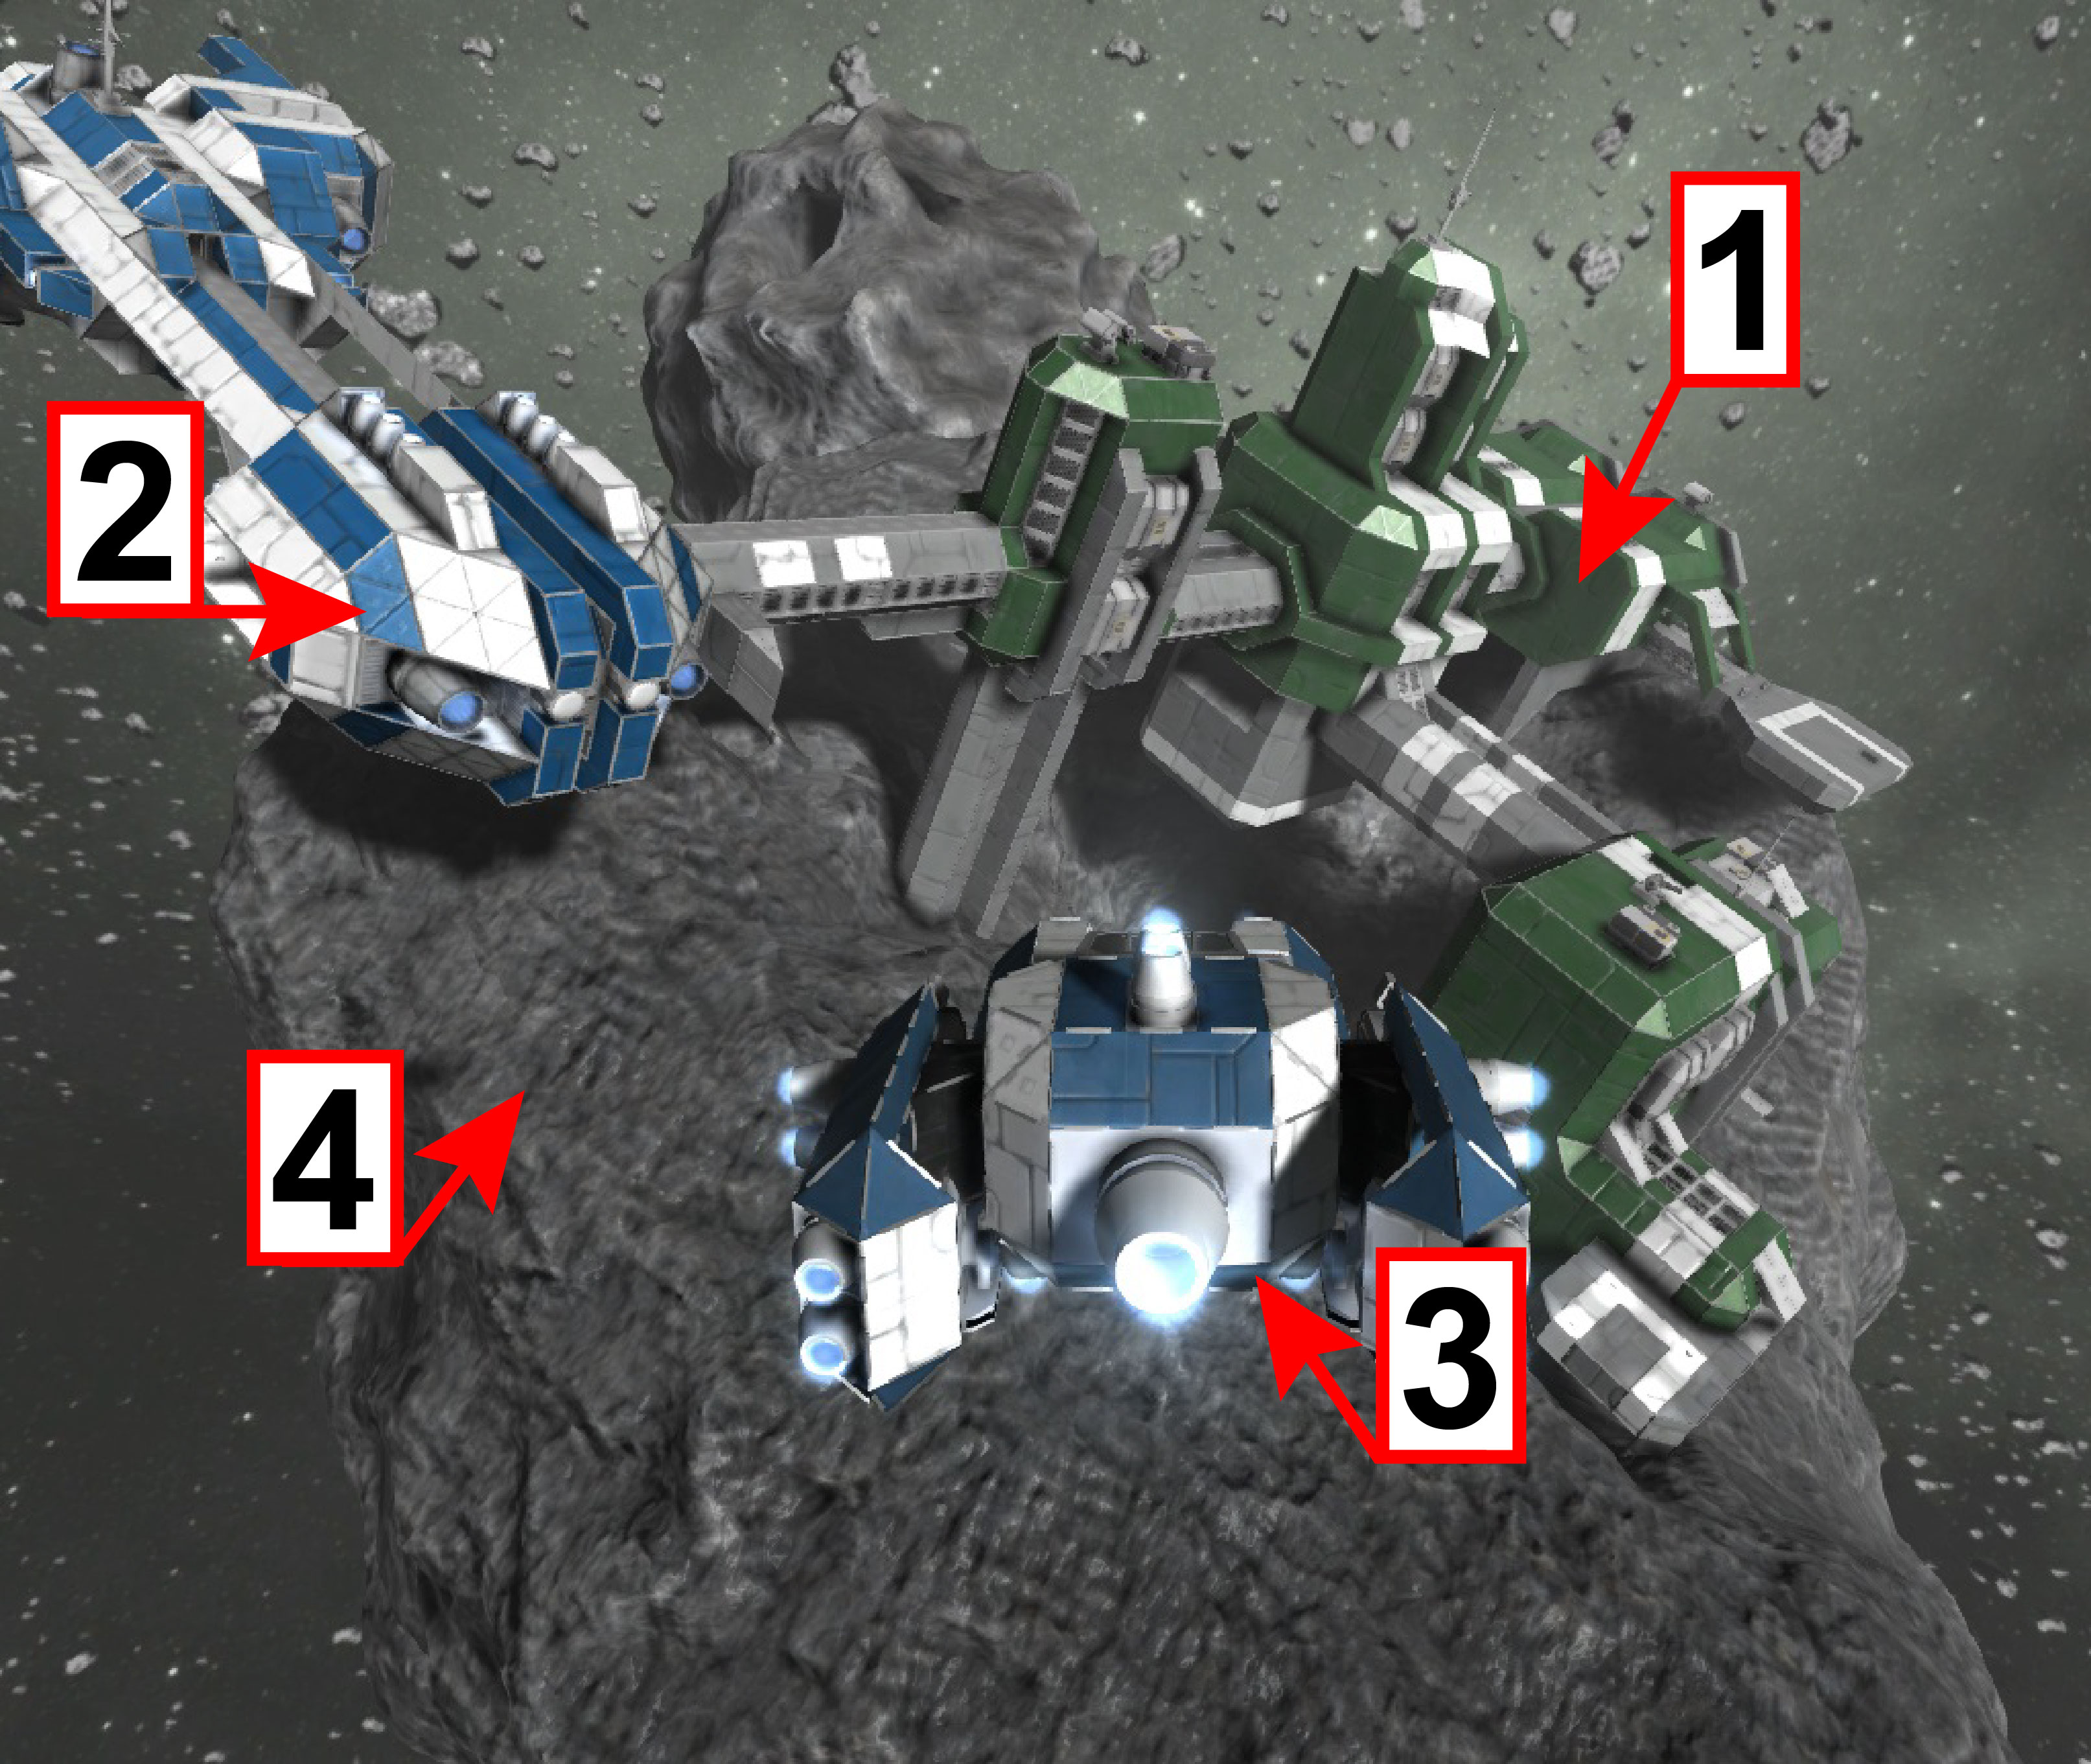
\includegraphics[ width=140mm]{../img/intro/se}

\caption{Hra Space Engineers -- základna. Zdroj: Gamespot.com \citep{se_intro_img} }
\label{fig:intro_se}

\end{figure}

\FloatBarrier

Samotná základna i~vesmírná plavidla (detailní pohled na jiné plavidlo je na obrázku \ref{fig:intro_se_ship}) jsou tvořeny bloky. Vizuální reprezentace bloku může být i~jiného tvaru než jen krychle -- to je možné vidět na obrázku \ref{fig:intro_se_blocks}). Barevně jsou zde zvýrazněny hranice bloků. Jak základny, tak vesmírné lodě (které jsou navíc oproti základnám pohyblivé) využívají tento systém. 

\SE{} umožňuje stavět pohyblivé stroje, které si hráč postaví z~herních bloků a~ty se pak chovají jako jedna entita. Stále je na ně však aplikována fyzika, takže je možné plavidlo poškodit, nebo dokonce zničit. Tento stupeň realismu od naší hry vyžadovat nebudeme. Budeme však chtít mít ve hře bloky, jejichž model není tvaru krychle. Stejně jako v \SE{} budeme chtít, aby bylo možné bloky rotovat v libovolném směru (u bloků, u kterých to bude dávat smysl).


TODO zmínit crafting, stavěnbí, conveyor systém

\begin{figure}[!ht]\centering
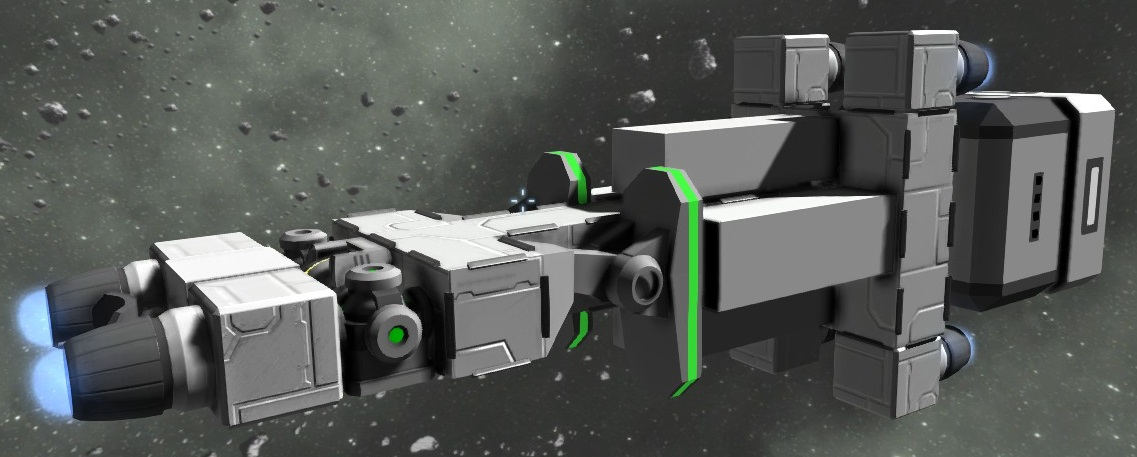
\includegraphics[ width=140mm]{../img/intro/se_ship}

\caption{Hra Space Engineers -- dron. Zdroj: space-engineer.net \citep{se_drone_source}}
\label{fig:intro_se_ship}

\end{figure}

\begin{figure}[!ht]\centering
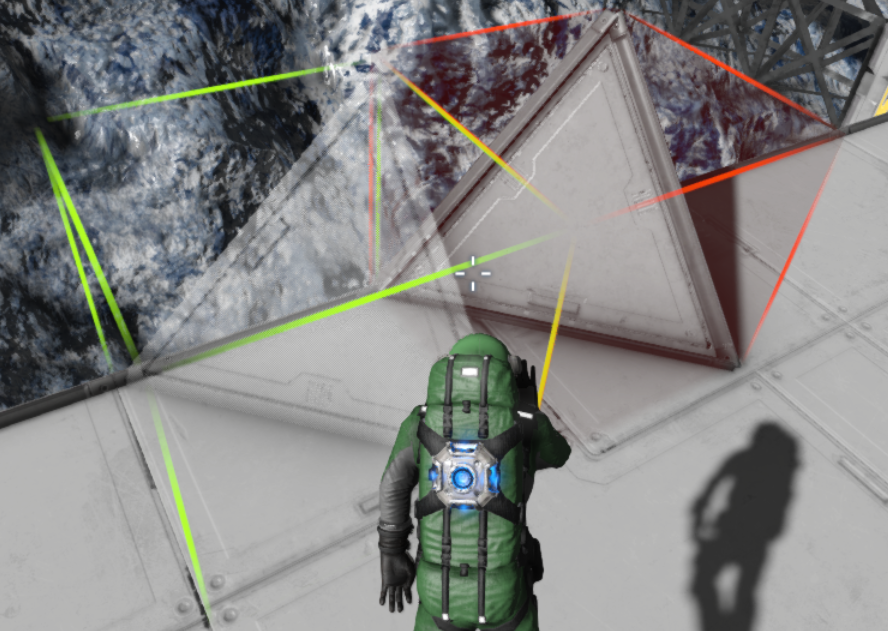
\includegraphics[ width=140mm]{../img/intro/se_blocks}

\caption{Hra Space Engineers - bloky }
\label{fig:intro_se_blocks}

\end{figure}

\FloatBarrier


\subsection{Hry s~maximálním důrazem na simulaci reality}

Do této sekce bychom měli zařadit například vesmírný simulátor \TM{}. // TODO popis, obrázek

Zmínit stavění

\begin{figure}[!ht]\centering
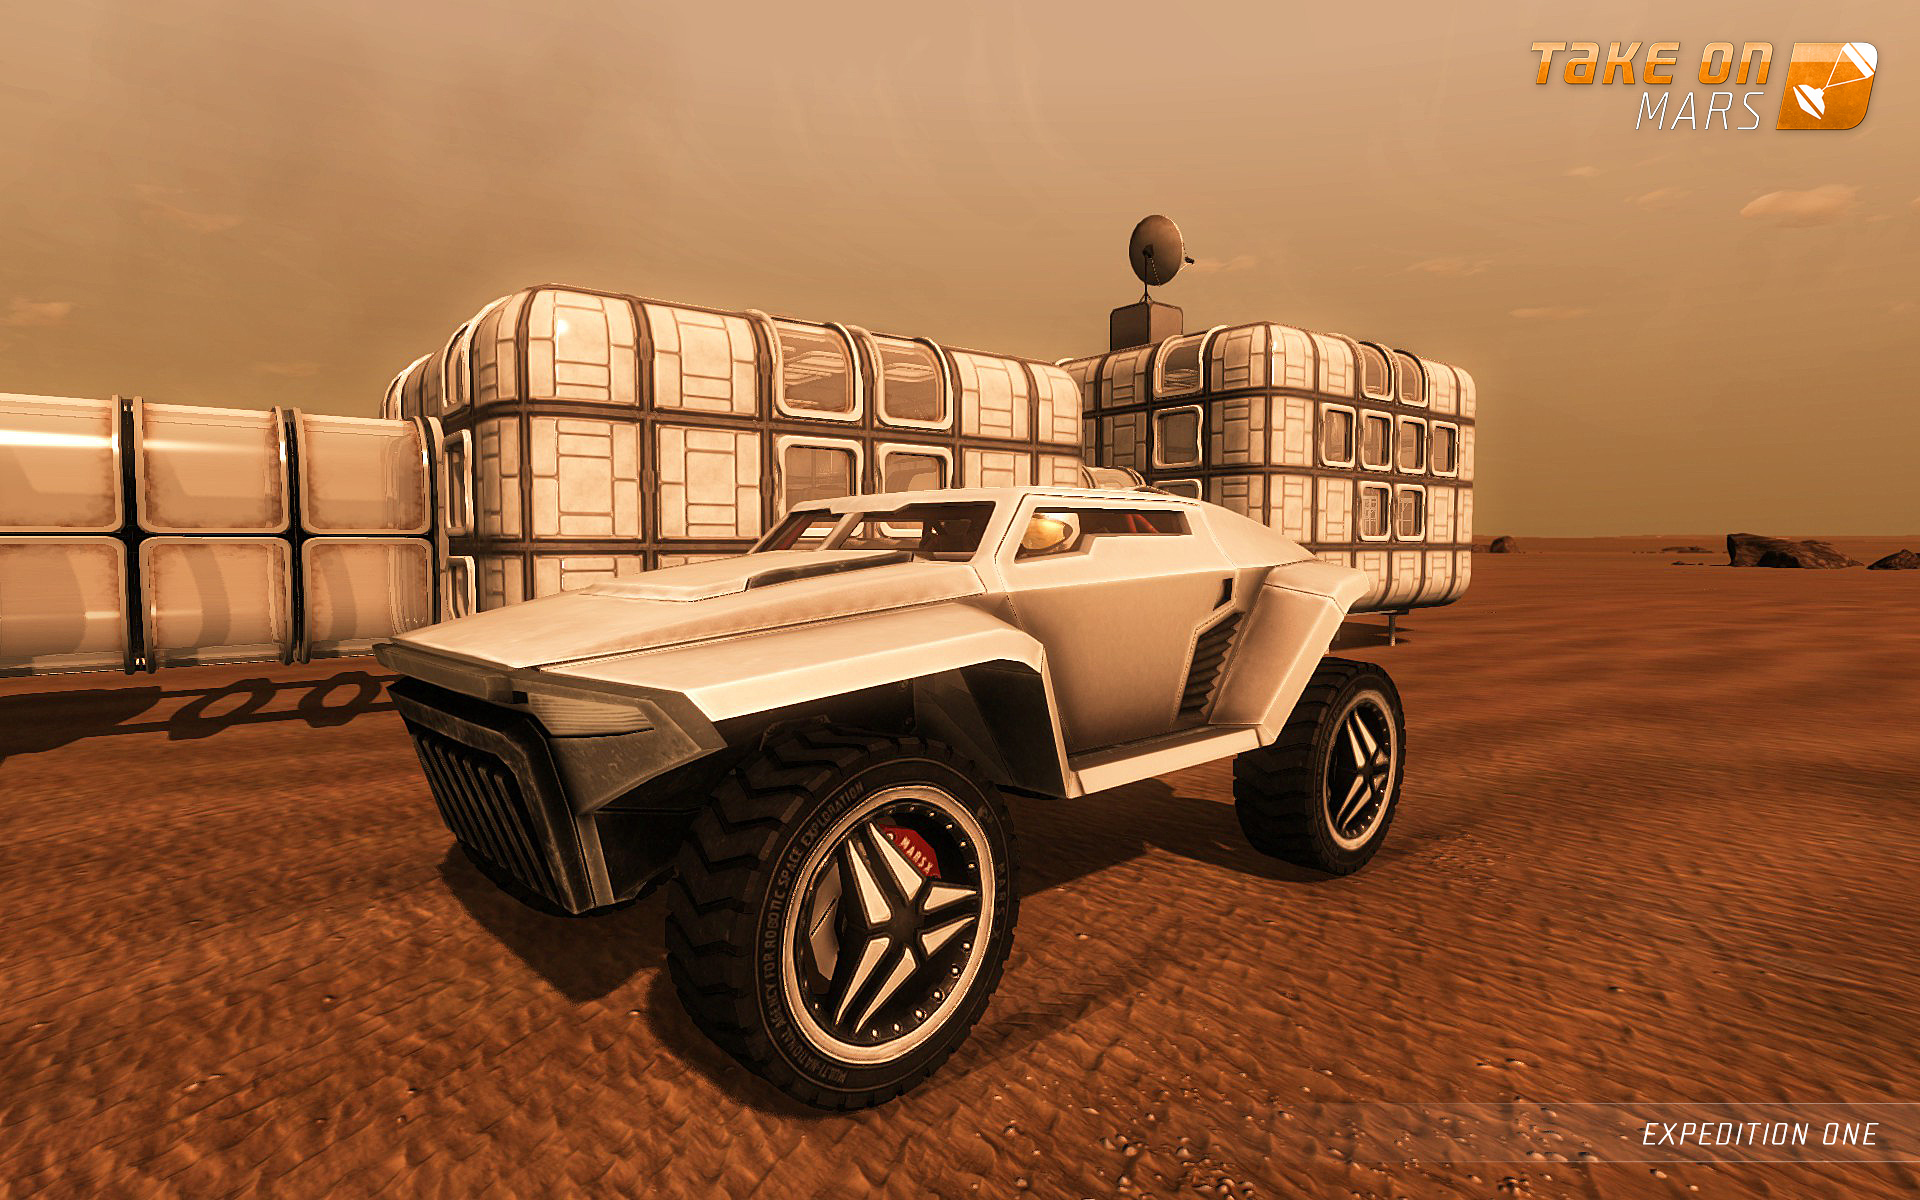
\includegraphics[ width=140mm]{../img/intro/tom}

\caption{Hry Take On Mars -- vozítko před budovou. Zdroj: Hry.cz \citep{intro_tom_source}}
\label{fig:intro_tom}

\end{figure}

\FloatBarrier

bloky na stavění, ale třeba vozidla kompletní

\subsection{Ostatní - zařadit TODO }

Můžeme však nalézt i~další příklady her (// TODO , , , , ).

\NI{}
Novus incpetio je MMORPG, stavění https://www.youtube.com/watch?v=d2ySkvn6wyw probíhá tím stylem, že se hráč přepne do build módu, vše si naplánuje (va výdledek vidí rovnou tak, jak bude vypadat). Po ukončení toho módu pak hráč vidí obrysy naplánovaných bloků. (Ty se přichytávají do mřížky a k sobě) Pak je může začít konstruovat, přičemž v nabídce během konstrukce má možnost si chybějící součásti craftnout.


\PN{}

https://www.youtube.com/watch?v=Wpurqr3YaGQ funguje podobně jako Space engineers - získávání surovin, kraftění na komponenty a použřívání komponent na konstrukci objetků. POstavený objekt ukazuje základní konstrukci.


\ARK{}
Ark počáteční free point, pak se bloky přidávají k sobě https://www.youtube.com/watch?v=TOmjjo5QoP8 


\NMS{}
Stejně jako \TM{} používá snappointy

\section{Čemu se budeme věnovat}

Rádi bychom zachovali koncept použití herních bloků, který shledáváme jednoduchý na pochopení i~použití. Zaměříme se na rozšíření možnosti práce s~bloky tak, abychom uživateli nabídli, pokud možno, ještě lepší herní zážitek ze stavění vlastních výtvorů. V této práci se nebudeme nijak důkladně věnovat vizuální reprezentaci prostředí, protože ta pro nás v~tuto chvíli není podstatná. 

Změna v~přístupu k~herním blokům bude vyžadovat i~úpravy herního mechanismu s~tím souvisejícího -- hráčova inventáře. Všechny výše zmíněné hry nějakým způsobem nabízí hráči výběr bloků, které může do herního světa umístit. Naše změna by bohužel znamenala, že by se takový inventář postavitelných bloků velmi rychle stal nepřehledným a~proto musíme systém nabídky postavitelných bloků upravit pro naše potřeby.

\section{Herní bloky}



Obvykle je ve hře definován jeden základní rozměr bloku, který je neměnný. (\SE{} definuje více velikostí -- ty však nelze vzájemně kombinovat). To však může být problémem, pokud se hráč rozhodne postavit v~herním světě nějakou větší a~komplexnější strukturu podle reálné či fiktivní předlohy. Pro příklad uveďme některé výtvory ze hry \MC{} -- město Královo přístaviště z~knih Píseň ledu a~ohně od Geoge R. R. Martina, nebo hlavní město Gondoru Minas Tirith z~knih Pána prstenů od J. R. R. Tolkiena.

Autoři těchto výtvorů museli volit takové měřítko, aby byly výtvory dostatečně detailní, ale zároveň aby bylo možné výtvor postavit v~nějakém rozumném čase. Obecně můžeme říct, že čím větších detailů chtějí autoři ve hře \MC{} dosáhnout, tím větší musí celý výtvor být. To pak ale znamená, že celá stavba trvá déle, nebo je zapotřebí více spolupracujících hráčů. Hra \SE{} díky svému přístupu a~více bloků, které nejsou tvaru krychle, nabízí lepší možnosti staveb rozsáhlých objektů (představme si třeba Hvězdu smrti z~Hvězných válek), ale stále je potřeba volit nějakou rozumnou výslednou velikost.


\subsection{Náš návrh úpravy}
Chtěli bychom se v~této práci zabývat myšlenkou proměnlivé velikosti stavitelných bloků. Tím by hráči mohli rychleji stavět rozsáhlejší struktury a~přitom se věnovat i~drobným či estetickým detailům. Tento návrh však s~sebou nese několik problémů, které se v~této práci budeme snažit vyřešit.


\section{Inventář}
Dalším společným prvkem tohoto druhu her je inventář bloků, které může hráč umístit do herního světa. Hráč přes celé herní okno vidí \HUD{} (Head-Up Display \citep{hud_terminology}), ve kterém má zobrazenou kromě jiného nabídku bloků, které má na rychlé volbě, může je snadno zvolit a~daný blok umístit do herního světa. Navíc hry mohou definovat i~inventární skupiny bloků (\SE{}, \ME{}), mezi kterými hráč může přepínat a~tím rychle kompletně změnit sadu rychlé nabídky. Vidíme však limitaci v~tom, že hráč musí ručně spravovat tyto seznamy a~jednotlivé bloky (či nástroje) umisťovat do příslušných pozic.


\subsection{Náš návrh úpravy}
Rádi bychom navrhli jiný způsob správy těchto inventárních skupin, aby hráč jednou definoval, jaké prvky chce mít v~příslušných skupinách. Při vytvoření nového bloku či vytvoření jiné velikosti bloku by pak nemusel ručně přiřazovat nový blok do skupiny, ale tento blok by měl být automaticky zařazen a~nabídnut hráči.  




\section{Cíle práce}
Tato práce by měla naplnit následující cíle:
\begin{itemize}
	\item Navrhnout a~implementovat způsob řešení proměnlivé velikosti bloků
	\item Navrhnout a~implementovat automatizovanou správu inventáře
	\item Kvůli očekávaným nárokům na pochopení nových konceptů do hry implementovat výukový tutoriál (TODO má to být tady?)
	\item Získat a~zhodnotit zpětnou vazbu na výslednou hru
\end{itemize}


%!TEX root = ../prace.tex

\chapter{Analýza zadání}

\section{Stávající implementace mechanismů}
- v dalším textu budeme vycházet z her: \\

Minecraft \\
Space Engineers / Medieval Engineers \\

\begin{itemize}
	\item popsat, jak je to v jednotlivých zmíněných hrách (musel jsem je nutně hrát všechny?)
	\item popsat velikosti bloků, nějaké zákonitosti, fyziku
	\item popsat strategické mechaniky
\end{itemize}

\section{Rozbor zadání}

Zde bychom měli popsat, co by se nám ve hře líbilo a stanovit reálnost implementace
\\

Nejspíše se text bude prolínat s kapitolou - dalším vývojem?\\
Měl bych si tu vysnit celou hru, nebo to spíše seškrtat?


\begin{itemize}
	\item tedy že bychom chtěli panďuláka, jaké pohledy
	\item a že bychom s ním chtěli chodit a stavět a bourat
	\item ale že nám taky může umřít - počasí, kyslík
	\item popsat svět, bloky, co by asi měly umět

\end{itemize}


\section{Cíle práce}
%!TEX root = ../prace.tex

\chapter{Detailní analýza}

V této kapitole podrobně rozebereme cíle práce. Už víme, čeho bychom chtěli dosáhnout a nyní potřebujeme vyřešit \textit{jak} toho dosáhnout.

%!TEX root = ../prace.tex

\section{Použitý herní engine}
- máme několik možností:

- napsat si vlastní (ne, moc práce)

- použít low level (XNA) - opět ne, moc práce

- Unity nebo Unreal Engine

- Unity mělo alespoň v době analýzy této práce problémy s dynamickým navmeshem, oproti tomu mělo editovatelný terén. Další nevýhoda je absance editorů materiálu tk jak je tomu v UE

- Unreal je prostě nej

%!TEX root = ../../prace.tex

\section{Bloky}

V této části rozebereme, jak můžeme definovat a~následně implementovat bloky a~popíšeme, jaké jsou výhody a~nevýhody jednotlivých implementací.\linebreak V~prvé řadě se zaměříme na celkovou strukturu bloků a~následně budeme řešit, jak budeme spravovat konstanty ovlivňující chování bloků.

\subsection{Celková struktura}

Aby se nám s~bloky dobře pracovalo, jistě bude vhodné využít jednoho ze základních principů \textit{OOP} (objektově orientovaného programování) -- dědičnosti. Takže v~naší hře bude existovat základní třída, která bude vycházet ze třídy \TT{UActor}\footnote{\TT{UActor} je základní třída \UEu{}, ze které dědí všechny herní objekty, které chceme v~hlavní herní smyčce aktualizovat a~renderovat.} a~bude předkem všech našich herních bloků. Tato třída by měla být kvůli rychlosti napsána v~\CPP{}.

Tento prapředek bude obsahovat dvě podstatné informace -- referenci na \textit{definici} daného bloku a~referenci na třídu s~vlastnostmi dané \textit{instance} bloku. Díky tomu, že oddělíme definiční třídu a~instanční třídu, tak získáme možnost získat definiční třídu pro daný typ bloku za běhu hry pouze jednou a~posléze tuto referenci předávat všem instancím bloku daného typu. Instanční třída bude mít pro každý blok jiné hodnoty, takže je zřejmé, že by měla být samostatná. Smyslem definičního souboru je popis omezujících podmínek kladených na daný typ bloku (například povolené minimální a~maximální rozměry), přičemž hodnoty v~instanční třídě by měly být v~mezích dané definicí. Vlastnosti, které nejsou omezující (například cena za postavení bloku), nebudeme uchovávat v~\textit{instanční} třídě, tyto údaje budeme získávat přímo z~\textit{definiční} třídy.

Pokud bychom zvolili jiný postup, snadno bychom si mohli \uv{svázat} ruce. Pokud by například \textit{instanční} vlastnosti byly vlastní součástí bázové třídy, systém ukládání hry by musel být schopen vidět a~pracovat minimálně s~touto bázovou třídou. Pokud však tyto vlastnosti vložíme do nějakého kontejneru (tedy třídy, která bude sloužit pouze jako přepravka pro data), tento kontejner klidně můžeme umístit do samostatného modulu\footnote{Moduly si lze představit jako samostatné knihovny, které se navzájem (acyklicky) referencují.}, nezávisle na modulu bloků a~modulu ukládání hry. Podrobněji se herním modulům věnujeme v~části \ref{sec:struct}.

\subsection{Instanční vlastnosti}
\label{subsec:instVlast}
Mezi instanční vlastnosti zařadíme vlastnosti definované v~části \ref{subsec:blocks} -- \textit{vizuální reprezentaci}, \textit{pozici ve světě}, \textit{rotaci}, \textit{velikost}, \textit{zdraví} apod. U~některých vlastností bychom navíc chtěli dosáhnout toho, aby konkrétní instance bloků měly rozdílné hodnoty dané vlastnosti v~závislosti na jejich velikosti. Jako ideu si můžeme představit následující: blok, který je větší než jiný blok stejného typu, bude mít více zdraví, protože je bytelnější a~více toho vydrží. Z~této úvahy nám zároveň vyplývá, že kromě rozměrů bloku se do výpočtu zapojuje i~typ bloku. Jako příklad uveďme fakt, že Zkosená krychle má oproti Krychli stejných rozměrů poloviční objem. Chceme dosáhnout nějaké úrovně realismu a~snadno nahlédneme, že cena za postavení těchto bloků (stejných rozměrů, ale různých typů) nemůže být stejná (ekvivalentně -- bylo zapotřebí poloviční množství materiálu k~výrobě jednoho bloku oproti druhému).

Z předchozího odstavce se tedy dostáváme k~algoritmu, kdy výsledná hodnota nějaké vlastnosti je pro danou instanci bloku počítána ze základní hodnoty (konstanty) pro daný blok, nějakého koeficientu dle typu bloku a~z~rozměrů bloku. Zadefinujme si následující konstanty pro daný \textit{typ}, vycházející z~objemu základní krychle: (jednotlivé hodnoty odpovídají sloupci \textbf{T} v~tabulce \ref{table:requiredBlocks})

\begin{enumerate}
	\item Krychle \textbf{K}: $1$
	\item Zkosená krychle \textbf{Z}: $\frac{1}{2}$
	\item Rohová krychle \textbf{R}: $\frac{1}{6}$
	\item Vlastní \textbf{V}: $1$
\end{enumerate}

Tyto konstanty využijeme v~následujícím algoritmu výpočtu

\begin{equation}\label{eq:alg}
	\bm H = \bm T * h * x * y * z
\end{equation}

kde $x, y, z$ jsou rozměry bloku v~daných osách, $\bm T$ je konstanta dle typu bloku, $h$ je nějaká základní hodnota dané vlastnosti (například zdraví) a~$\bm H$ je výsledná hodnota vlastnosti. Výpočet \ref{eq:alg} se opírá o~následující fakta:

\begin{enumerate}
	\item Blok, který je typu \textbf{V}, má vždy pevně definované rozměry a~nelze jej škálovat.
	\item Blok, který je typu \textbf{V}, do rovnice vždy dosazuje $ x = y = z~= 1$.
	\subitem To je čistě designová záležitost, abychom mohli během zadávání konstant pro daný blok tohoto typu vždy zadat pouze výslednou hodnotu. Vyhneme se tím přepočítávání a~zadání konstant bude přehlednější.
\end{enumerate}

Díky algoritmu \ref{eq:alg} tak může herní designér snadno nastavovat základní koeficienty vlastností a~hra bude výsledné hodnoty vlastností za běhu upravovat dle konfigurace hráčem postaveného bloku.


%!TEX root = ../../prace.tex



\section{Komponenty bloků}
\label{sec:komponents}

Nyní přistoupíme k~řešení problému rozšiřování funkcionality bloků. Z~analýzy v~části \ref{subsec:bloky} vyplývá, že některé bloky mají mj.~elektrickou komponentu, některé mají kyslíkovou komponentu a~jeden z~nich má obojí. Tradiční přístup \textit{OOP} nám nabízí použití rozhraní či dědičnosti. Práce s~rozhraním není v~\UEu{} nikterak jednoduchá, takže bychom rádi našli snazší cestu. Ačkoliv \CPP{} umožňuje vícenásobnou dědičnost, \UE{} ji kvůli svým kompilačním nástrojům nepovoluje. Navíc by bylo velmi těžké vymyslet takovou hierarchii dědičnosti bloků, abychom splnili požadavky pro všechny bloky a~přitom si zároveň neuzavřeli cestu pro implementaci nových bloků. 

Jednou z~dalších možností, jak problém sdílené funkcionality řešit, je systém \textit{komponent}, který nám \UE{} nabízí. Komponenta je programová část, která ovlivňuje chování vlastníka dané komponenty. Cílem je pak dosáhnout toho, že je možné za běhu hry jednu komponentu transparentně vyměnit za jinou (komponentu s~jinou implementací), a~vlastník komponenty se nemusí zajímat o~detaily implementace. Díky tomu je možné snadno rozšiřovat vlastnosti a~chování vlastníků dané komponenty.

Z předchozí analýzy vyplývá, že budeme potřebovat řešit následující problémy:

\begin{itemize}
	\item Práce s~kyslíkem
	\item Práce s~elektrickou sítí a~energií
	\item Interakce s~uživatelem
	\item Umístění bloku v~herním světě
\end{itemize}


Tyto problémy jsou ideální kandidáti na použití komponent. Pokud bychom se někdy v~budoucnu rozhodli upravit chování některé funkcionality či jej z~libovolného důvodu změnit, komponentový systém pro nás bude výhodou. Navíc ne všechny herní bloky umí (z hlediska herního designu) kupříkladu s~kyslíkem či elektřinou pracovat. Jak jsme již zmínili dříve,  s~použitím komponent to bude snadné -- bloky, které danou funkcionalitu mají umět, budou mít danou komponentu a~budou s~ní moci pracovat. Taktéž tím u~kyslíku a~energie získáme možnost přiřadit tyto komponenty hráčově postavě a~tím nebudeme duplikovat funkcionalitu.

\subsection{Komponenta kyslíku}

Cílem komponenty kyslíku by mělo být udržování informace o~aktuálním množství \uv{vlastněného} kyslíku a~dále pak převody mezi jednotlivými komponentami. V~rámci herního designu jsme se rozhodli, že kyslík bude ve hře vyráběn z~elektrické energie. Z~toho nám vyplývá, že kupříkladu blok s~elektrickou a~kyslíkovou komponentou musí mít možnost provádět převody zdrojů a~tedy bude moci měnit množství vlastněného kyslíku ve prospěch či neprospěch jiné kyslíkové komponenty (například té, kterou bude vlastnit blok \nameref{blocks:B10}). 



Obdobně jako u~bloků, kyslíková komponenta bude obsahovat reference na \textit{definiční} třídu a~\textit{instanční} třídu a~jejich chování bude vycházet z~principů chování definiční a~instanční třídy u~vlastností bloků. \textit{Definiční} třída bude definovat \textit{maximální objem drženého kyslíku} pro daný blok (a stejně jako u~výpočtu zdraví se pro danou instanci bloku použije algoritmus \ref{eq:alg}). Dále bude definovat \textit{maximální přenesený objem kyslíku za 1~herní sekundu}. Z~toho vyplývá, že budeme mít možnost řídit, jak dlouho bude probíhat přenos třeba z~bloku Plničky kyslíkových bomb do bloku Kyslíkové bomby, nebo z~bloku Kyslíkové bomby k~herní postavě hráče. Od této limitace přenosu si slibujeme, že hráčům přinese  věrohodnější herní zážitek. 

\subsection{Komponenta energie}

Komponenta energie by měla být v~mnohém velmi podobná Kyslíkové komponentě. Měla by udržovat informace o~\uv{vlastněné} energii a~taktéž by měla obsahovat reference na \textit{definiční} a~\textit{instanční} třídu. \textit{Definice} pro daný blok by měla obsahovat \textit{maximální objem} a~\textit{limit přenosu}. 

Navíc bychom chtěli, aby Energetická komponenta uměla pracovat s~\textit{elektrickou sítí}. Aby byla komponenta v~nějaké elektrické síti, musí se blok vlastnící tuto komponentu dotýkat jiného bloku s~elektrickou komponentou. Protože vycházíme z~reálného světa, tento dotyk vlastně simuluje vodivý spoj. Proto musíme pro každý blok s~touto komponentou umět zadefinovat, jak takový vodivý spoj vypadá.

\subsubsection{Vodivé spojení bloků}

Nejprve bychom měli zadefinovat pojem \textit{vodivý spoj} a~také zmínit jeho vlastnosti. V~naší hře budeme jako \textit{vodivý spoj} chápat propojení bloků skrze netriviální plochu. Tedy dvě stejně velké krychle mohou být vodivě spojeny, pokud mají společný dotyk jejich stěn alespoň o~velikosti stěny jednotkové krychle. Pokud se budou dotýkat hranami, nebo dokonce jen rohy, nebude toto postavení bráno jako vodivý spoj.

Pro implementaci bychom mohli použít (stejně jako u~stavění ve hře \TM{}) systém přípojných bodů. Nicméně to by znamenalo, že bychom museli řešit, jak tento systém upravit pro dynamicky škálovatelné bloky. Navíc, pro nové vizuální reprezentace bloků bychom museli speciálně řešit umístění těchto přípojných bodů, i~vzhledem k~ostatním možným přípojným bloků ve hře). Další zásadní nevýhodou tohoto návrhu je způsob, jak bychom napojovali například krychle o~maximálním a~minimálním rozměru. Abychom mohli využít přípojných bodů, minimální krychle by musela definovat $6$ takových bodů a~maximální krychle pak $2~400$ těchto bodů. S~rostoucí velikostí bloku se počet kontrolovaných přípojných bodů zvětšuje a~obáváme se, že výpočetní algoritmy by mohly být při kontrole velmi pomalé.  Tento postup nám nevyhovuje.



Můžeme však zvolit obdobné řešení -- \uv{\textit{polygonální}}. Pro daný blok definujeme \textit{body}, které se budou v~rámci škálování korektně umisťovat vždy na stejné místo (například roh krychle). Dále pak definujeme \textit{polygony}, což je uspořádaný seznam bodů, které leží v~dané rovině. Tento seznam tvoří virtuální cyklus, takže mezi $k$-tým a~$(k+1)$-tým bodem je \textit{hrana} polygonu. Konceptuální náhled této myšlenky je vidět na obrázku \ref{fig:polygons}.

\begin{figure}[!ht]\centering
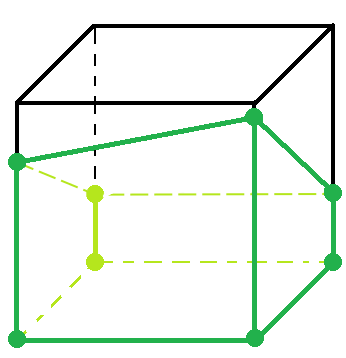
\includegraphics[ width=70mm]{../img/analysis/krychle}

\caption{Příklad nastavení polygonů}
\label{fig:polygons}

\end{figure}

\FloatBarrier

Obrázek \ref{fig:polygons} nám dává náhled nějakého možného uspořádání pěti polygonů v~rámci krychle. Silně vykreslené body představují definiční \textit{body}, jednotlivé čáry pak \textit{hrany} polygonů. Záměrně jsme neudělali polygony pravidelné, abychom demonstrovali, že je možné se libovolně přizpůsobovat tvarům vycházejícím z~polygonální reprezentace daného bloku.


V rámci algoritmu spojování bloků skrz vodivé spojení pak budeme hledat pro daný blok sousedy právě dle těchto definic. Budeme počítat s~tím, že polygony jsou v~rámci jedné roviny v~prostoru, přičemž daná rovina je rovnoběžná s~některou z~rovin mřížky herního světa. V~rámci této práce si algoritmus usnadníme takovým způsobem, že jednotlivé studované polygony rozšíříme na \textit{boxy}, tedy najdeme nejmenší možný kvádr, který je zarovnaný do mřížky definované herním světem (tedy nemá vůči ní žádnou rotaci) a~obsahuje všechny body z~daného polygonu\footnote{Abychom mohli použít standardních metod \TT{FBox::Intersect(...)}, musíme \textit{box} rozšířit o~něco netriviálního (např. $1~cm$) ve směru normály dané roviny.}. Za validní a~vodivé elektrické vedení pak budeme považovat takové dva polygony, které mají neprázdný průnik těchto boxů. Jsme si vědomi faktu, že tato úprava jde proti snahám hry o~vyšší stupeň realismu a~pro některé kombinace bloků dokonce bude porušovat naši definici vodivého spojení, ale v~této fázi nám to stačí a~nebudeme vyžadovat matematicky správné řešení.


\subsection{Objekt elektrické sítě}

Spojování bloků do elektrické sítě nevyžaduje žádnou speciální logiku. V~rámci přidávání bloku do herního světa budeme potřebovat vědět o~sousedních blocích (TODO stromy). Pokud bude vazba se sousedním blokem vyhodnocena jako validní vodivý spoj, může se nově připojený blok připojit ke stávající síti, v~níž je i~daný sousední blok.

Pokud budeme vycházet z~premisy, že každý blok je zapojen právě v~jedné elektrické síti a~všechny bloky v~rámci jedné elektrické sítě jsou mezi sebou vodivě spojeny, tak nutně musíme dojít k~závěru, že při manipulaci s~blokem budeme muset elektrické sítě aktualizovat. Přidáním bloku jsme bychom mohli vodivě propojit dvě či více sítí, při odebírání se nám daná elektrická síť může rozpadnout na více samostatných komponent. Těchto elektrických sítí může vznikat a~zanikat velké množství. Stačí si uvědomit, že k~bloku \nameref{blocks:A1} o~maximální možné velikosti můžeme připojit až 600 bloků, které budou patřit do stejné sítě (pro každou stěnu máme 100 bloků stejného typu a~minimální velikosti, uspořádaných do šachovnicového vzoru). Pokud pak odebereme centrální blok, může nám vzniknout právě až 600 nových elektrických sítí. Navíc, díky počasí se může stát, že bloky budou odebírány ze světa zcela neuspořádaně (na základě náhodně udělovaného poškození). Musíme tedy vymyslet algoritmus, jak pro všechny bloky v~herním světě udržovat správné informace o~jejich síti.

Protože nemůžeme nic předpokládat o~tom, jak se budou bloky v~elektrické síti chovat, musíme při změně (přidání či odebrání) nějakého bloku v~síti provést přepočítání. Nejjednodušší bude varianta na \textit{algoritmus vlny}. Jednotlivé sítě budeme podle potřeby odstraňovat či slévat. Popišme si nyní pravidla, která budeme muset ve hře mít. Jako sousedy budeme chápat bloky dostupné skrze vodivé spojení.

\subsubsection{Přidávání bloku}
Platí, že každý blok přidaný do herního světa si vytvoří svoji vlastní elektrickou síť.
(TODO kontrola enums níže)
\begin{enumerate}
	\item Pokud blok nemá žádné sousedy, nemusí dělat nic (svoji síť už má)
	\item Pokud mají všichni sousedé stejnou síť, blok se k~ní připojí
	\item Pokud mezi sousedy existují alespoň dvě různé elektrické sítě, blok si vytvoří novou elektrickou síť, propojí ji s~ostatními sítěmi a~vyvolá přepočet sítí
\end{enumerate}

\subsubsection{Odebírání bloku}
Platí, že každý odebíraný blok z~herního světa vždy odstraní síť, ve které je připojen, a~pro všechny jeho sousedy jsou vytvořeny nové sítě.

\begin{enumerate}
	\item Pokud blok nemá žádné sousedy, svoji síť ze hry odstraní a~dále nedělá nic
	\item Pokud má blok právě jednoho souseda, odpojí od se od dané sítě
	\item Pokud má alespoň dva sousedy, pro každého vytvoří novou síť a~vyvolá přepočet sítí
\end{enumerate}

\subsection{Udržování konzistence elektrických sítí}

Jak je vidět z~předchozí kapitoly, objektů k~aktualizaci může být velmi mnoho. Nesmíme však dopustit, aby se nám při přepočítávání začala hra zpomalovat či přímo zasekávat\footnote{Tato situace může snadno nastat, protože herní a~renderovací smyčky se na konci svých cyklů synchronizují, aby pro výpočet dalšího framu začínaly stejně.}. Opět máme více možností řešení, jak se k~tomuto problému postavit. 

Jedním z~možných řešení je spuštění výpočtů na samostatném výpočetním vlákně. Zde bohužel narážíme na problém, že výpočty ve vláknech v~\UEu{} nemohou přímo přistupovat k~herním objektům a~tudíž je nutné používat pomocných datových struktur a~výsledky poté zpětně propagovat. Kromě toho také narážíme na problém, kdy v~případě velmi silné bouře kyselých dešťů bude nejspíše často nutné výpočet předčasně ukončit a~spustit znovu.

My navrhujeme následující algoritmus, využívající front požadavků ke zpracování a~omezení výpočetního času. Ještě musíme zmínit, že také využívá toho, že jak elektrická síť, tak každý blok v~ní si nese informaci o~stavu. Ty jsou tři:
\begin{itemize}
	\item Nevalidní
	\item Ve výpočtu
	\item Validní
\end{itemize}
Volba stavů je zřejmá a~vychází z~principů algoritmu vlny. Dalším netriviálním faktem je, že v~algoritmu existuje fronta sítí k~přepočítání, přičemž každá taková má svoji frontu bloků v~síti k~přepočítání. Hlavním krokem algoritmu je pak výběr sítě k~přepočítání a~provedení jednoho kroku přepočtu. Následně, pokud má tato síť stále nějaké bloky k~přepočtu, je zařazena na konec přepočítávací fronty a~tam čeká, dokud nebude opět vyzvednuta. Může se však stát, že jistou posloupností kroků při mazání bude tato síť označena jako nevalidní a~dále se přepočítávat nebude.

Algoritmus bude mít přidělené nějaké maximální kvantum času, řekněme tak, aby při jeho výpočtech hra dosahovala alespoň 30 snímků za sekundu. Tím vcelku jednoduchým a~elegantním způsobem zajistíme přepočty i~pro velice rozsáhlé sítě. Samozřejmě je nutné, aby hra počítala s~tím, že elektrická síť a~bloky v~ní mohou být ve stavu \textit{ve výpočtu} a~tomu přizpůsobovat další funkcionalitu (například nevyužívat zdrojů takovéto sítě, dokud blok není \textit{validní} -- pak je možné využívat pouze dalších validních bloků, tedy těch, které již byly zpracovány algoritmem).

TODO tabulka případů, říct, že tohle bude komponenta

\subsection{Interakce a~označování}
\label{subsec:interaction}

Dalším problémem je interakce s~uživatelem. Abychom věděli, že hráč s~daným blokem chce interagovat, musíme vědět, že:
\begin{itemize}
	\item Je dostatečně blízko bloku
	\item Z~pohledu hráče se dívá na daný blok 
	\item Vyjadřuje fakt, že chce interagovat (např. stiskem klávesy)
\end{itemize}



Nejsnazší způsob, jak zjistit, na jaký herní objekt se hráč dívá, je použití techniky sledování paprsku (\textit{ray tracing}). Díky němu můžeme \uv{z kamery} vyslat virtuální paprsek, který má stejný směr, jako je směr pohledu kamery. Pokud bude hráčův \HUD{} zobrazovat zaměřovací kříž (či použijeme nějaký obdobný mechanismus) a~náš paprsek bude z~pohledu kamery tímto zaměřovačem procházet, hráč může cíleně mířit na herní objekty a~my zároveň budeme mít správnou informaci o~objektu, na který hráč zaměřovačem míří. Tento způsob získávání informace o~objektech v~hráčově zaměřovači je ve hrách běžný a~jeho použití je (pokud je vhodně použito) i~dostatečně rychlé.

Nyní, když už víme, jak můžeme získávat informace o~tom, na který objekt hráč míří, tak tento mechanismus ještě rozšíříme o~další vlastnost. Je zapotřebí si uvědomit, že interakce s~blokem a~umisťování nového herního bloku (případně mazání) jsou prakticky stejné akce. Liší se pouze výsledkem -- reakcí na stisk nějaké klávesy či tlačítka myši. Ale ve všech případech musíme vědět, na jaký blok hráč míří zaměřovačem, u~umisťování navíc potřebujeme znát i~přesný polygon, na který hráč míří. Konkrétní polygon potřebujeme znát z~toho důvodu, že chceme, aby se přidávaný blok \uv{přilepil} k~bloku, na který míříme. Tedy chceme zachovat herní mechaniku, která je v~hrách z~kapitoly \ref{chap:uvod} běžná a~je natolik intuitivní a~rozšířená, že změna této mechaniky by nejspíše nedopadla dobře a~hráči by nebyla kladně přijata.

Pro implementaci nám poslouží metoda \TT{LineTraceSingleByObjectType},\linebreak které předáme správné parametry (především počátek a~konec paprsku a~typy objektů, které paprsek zaznamená) a~ta nám vrátí strukturu, popisující výsledek trasování. Z~něj se můžeme dozvědět, jestli byl nějaký blok v~cestě paprsku. A~pokud ano, můžeme se ptát, zda měl komponentu interakce (potenciálně bychom mohli chtít bloky bez možnosti zaměření a~interakce, jakožto nesmazatelné objekty). Pokud bude i~tato podmínka splněna, můžeme se zajímat o~další vlastnosti kolize paprsku s~blokem a~na základě toho se nějak chovat.

Abychom hráči hraní usnadnili a~zpříjemnili, budeme bloky zvýrazňovat za použití techniky \textit{obrysu} (implementace zvýrazňování bude vycházet z~tutorialu~\citep{ue_outline_tut}). Tato technika je také využívána v~různých hrách napříč různými herními žánry a~proto její implementací nic nezkazíme. Obrys zobrazíme v~případě, kdy hráč nic nestaví a~daný označený blok je použitelný (takže hráč ví, že blok může používat), nebo v~případě, kdy hráč staví (zvýrazníme hranice namířeného objektu). Barvu obrysu můžeme zvolit kupříkladu zelenou pro použitelný blok, žlutou při stavění a~červenou při odebírání bloku. 


\subsection{Umístění ve světě}

Smyslem této komponenty je oddělení implementace bloku jako takového a~implementace herního světa. Skrze tuto komponentu se blok bude moci dotazovat na ostatní bloky v~herním světě, především pak bloky ve svém okolí. To bude důležité například pro elektrickou komponentu, která na základě \uv{sousedství} bude jednotlivé bloky vázat k~sobě do elektrické sítě.








\section{Definice bloků}
\label{sec:db}

Jak bylo řečeno v~analýze v~části \ref{sec:chceme}, potřebujeme u~bloků definovat mj.~následující vlastnosti: \textit{minimální} a~\textit{maximální} velikost, \textit{typ} bloku, možnost \textit{rotace} bloku dle daných os apod. Dále budeme u~bloků potřebovat zaznamenat, že blok má \textit{elektrickou} či \textit{kyslíkovou} komponentu a~definovat omezující vlastnosti této komponenty. Dále požadujeme, abychom mohli snadno modifikovat hodnoty těchto vlastností. Tento požadavek vznášíme z~toho důvodu, aby herní designér mohl rychle a~jednoduše ladit nastavení těchto konstant a~vyvažovat tak celkovou obtížnost hry. Takže nepřipadá v~úvahu, abychom měli tyto konstanty uložené ve zdrojovém kódu, protože jakákoliv úprava by znamenala opětovnou kompilaci hry a~to u~herních projektů často zabere netriviální čas. Pak je ale budeme muset načítat z~nějakého souboru, nebo budou muset být uložené v~nějakém definičním objektu, editovatelným z~Editoru.


\subsection{Textové soubory}
Při načítání definic z~textového souboru máme na výběr z~více možností. V~následujících odstavcích si jednotlivé možnosti popíšeme a~zamyslíme se nad výhodami a~nevýhodami daných přístupů. Jednu výhodu však mají všechny textové přístupy společnou -- snadnou čitelnost i~pro běžného člověka.

\subsubsection{Popis tabulkou}
Uvažme popis bloků v~nějakém tabulkovém formátu, třeba CSV. Pokud\linebreak bychom měli velice málo vlastností bloků, tento přístup by mohl být použitelný. Nicméně s~každým dalším nově přidaným blokem se do množiny všech vlastností mohou zanášet nové vlastnosti. To by znamenalo, že popis ostatních bloků, které danou vlastnost nemají, by musel nutně v~tomto tabulkovém zápisu uvažovat nějakou (byť prázdnou) hodnotu. Zbytečně by nám tak rostl definiční soubor. Další nevýhodou je absence typové bezpečnosti pro uložené hodnoty. 

\subsubsection{Popis samostatným souborem -- XML}
Běžné soubory textového formátu (TXT) není potřeba brát v~potaz. Výsledek je stejný jako při použití XML, ale nemůžeme zde použít definiční soubory pro automatickou kontrolu platnosti hodnot. Navíc bychom museli psát vlastní parser takového textového souboru, přičemž již hotové parsery XML jsou volně k~dispozici a~mohli bychom je snadno použít. Definici herních bloků v~XML využívá i~hra \ME{}. Tyto soubory jsou pak zpracovány herním enginem během načítání hry. Výhodou tohoto přístupu je, kromě snadného vytváření módu do hry, také snadná budoucí rozšiřovatelnost o~nové bloky.

\subsection{Binární zápis}
Binární zápis již není pro běžného člověka tak snadno čitelný, ale to nám nemusí vadit, pokud budeme mít k~dispozici příslušné editační rozhraní. My si totiž můžeme v~\UEu{} připravit třídu, jejíž vlastnosti jsou z~Editoru editovatelné pouze v~rámci nastavování výchozích hodnot. To znamená, že si na straně \CPP{} můžeme vhodným způsobem vytvořit strukturu definičních tříd, které následně použijeme v~Editoru. Na straně \UEu{} pak vytvoříme Blueprint, který bude dědit z~naší hlavní definiční třídy. Posléze můžeme této třídě upravovat výchozí hodnoty a~tímto způsobem tak definovat vlastnosti bloků.

Kromě toho, že tímto přístupem splňujeme požadavek na editovatelnost z~Editoru, získáváme také navíc typovou bezpečnost uložených hodnot. Dále máme možnost (v případě nějakých definičních specialit) vytvořit vlastní editační panely pro dané netriviální vlastnosti definičního souboru. 


\subsection{Definice bloků -- verdikt}

Na základě výše zmíněných poznatků jsme se rozhodli, že budeme bloky definovat v~binárním formátu. V~\CPP{} implementujeme definiční třídu s~vhodnou strukturou a~v~Editoru pak následně vytvoříme Blueprintové assety, ve kterých požadované vlastnosti pro námi požadované bloky nadefinujeme. Získáme tak možnost snadné úpravy požadovaných vlastností v~Editoru a~typovou bezpečnost vyplněných hodnot.

%!TEX root = ../../prace.tex


\section{Elektrická síť}
\label{sec:energyNet}
Účel elektrické sítě ve hře vychází z~reálného světa. Chceme, aby bloky spolu mezi sebou uměly komunikovat skrze nějakou síť a~aby přes tuto síť bylo možné automaticky převádět energii, třeba z~bloku \RB{B6} do bloku \RB{B8}. Na elektrickou síť nebudeme klást žádné omezující požadavky (například limitací přenosové kapacity bloků tvořících danou síť).

Pokud budeme vycházet z~premisy, že každý blok je zapojen právě v~jedné elektrické síti a~všechny bloky v~rámci jedné elektrické sítě jsou mezi sebou vodivě spojeny (viz kapitola \ref{subsec:encomp}), tak nutně musíme dojít k~závěru, že při manipulaci s~bloky budeme muset elektrické sítě aktualizovat. Přidáním bloku bychom mohli vodivě propojit dvě či více sítí, při odebírání se nám daná elektrická síť může rozpadnout na více samostatných komponent. Těchto elektrických sítí může vznikat a~zanikat velké množství. Stačí si uvědomit, že k~bloku \RB{A1} o~maximální možné velikosti můžeme připojit až 600 bloků, které budou patřit do stejné sítě (pro každou stěnu máme 100 bloků stejného typu a~minimální velikosti, uspořádaných do šachovnicového vzoru). Pokud pak odebereme centrální blok, může nám vzniknout právě až 600 nových elektrických sítí. Navíc, díky počasí se může stát, že bloky budou odebírány ze světa zcela neuspořádaně (na základě náhodně udělovaného poškození). Musíme tedy vymyslet algoritmus, jak pro všechny bloky v~herním světě udržovat správné informace o~jejich síti.

Protože nemůžeme nic předpokládat o~tom, jak se budou bloky v~elektrické síti chovat, musíme při změně (přidání či odebrání) nějakého bloku v~síti provést přepočítání a~to i~u~sítě, která již může být přepočítávána. Nejjednodušší bude varianta na \textit{algoritmus vlny}. Jednotlivé sítě budeme podle potřeby odstraňovat či slévat. 


Aby algoritmus vlny fungoval, je zapotřebí u~elektrické sítě a~každého bloku v~ní udržovat informaci o~stavu. Ty jsou tři:
\begin{itemize}
	\item Nevalidní
	\item Ve výpočtu
	\item Validní
\end{itemize}

Volba stavů je zřejmá a~vychází z~principů algoritmu vlny. Navíc tím můžeme požadovat, aby hra počítala s~tím, že elektrická síť a~bloky v~ní mohou být v~různých stavech a~tomu pak přizpůsobila svoji další funkcionalitu (například síť ve stavu \textit{ve výpočtu} nebude převádět zdroje sítě mezi bloky, které nejsou ve stavu \textit{validní} -- tedy těch, které již byly zpracovány algoritmem).

\subsection{Princip aktualizace sítě}

V předchozí části jsme zjistili, že nám může v~jednom okamžiku vzniknout velké množství sítí, jež je třeba aktualizovat. Navíc platí, že sítě mohou být rozsáhlé. Abychom co nejméně zasahovali do funkcionality aktualizovaných sítí, musíme nějakým způsobem zajistit, aby byla aktualizace sítí férová pro všechny sítě k~aktualizaci. Vzhledem k~tomu, že při nově vzniklém požadavku na aktualizaci sítě nevíme vůbec nic o~tom, které bloky nakonec v~dané síti budou, nemá smysl se zabývat myšlenkou upřednostňování aktualizace nějaké sítě vůči jiné, protože nemáme žádné faktické podklady pro to, jakou síť bychom měli upřednostnit.

Musíme tedy mít k~dispozici \textit{frontu sítí k~aktualizaci}. Každá síť z~této fronty si pak bude muset držet \textit{vlastní} frontu \textit{bloků k~aktualizaci}. V~algoritmu budeme postupně z~fronty vybírat sítě, provedeme u~nich krok algoritmu vlny a~případně je opět zařadíme do fronty. Tím zajistíme férovou aktualizaci pro všechny zúčastněné sítě.

Dále popíšeme, jak vypadá jeden krok algoritmu vlny. Jako sousedy budeme chápat bloky dostupné skrze vodivé spojení. Krok bude následující:

\begin{enumerate}
	\item Vyber blok \textbf{B} z~fronty bloků k~aktualizaci.
	\item Zkontroluj, že je \textbf{B} stále validní (zatímco \textbf{B} čekal ve frontě, mohl být mezitím zničen bouří kyselého deště). Pokud není validní, skonči.
	\item \textbf{B} označ jako \textit{Validní}.
	\item Pro všechny sousedy \textbf{S} bloku \textbf{B} se podívej na jejich síť a~stav bloku a~vykonej akci dle tabulky \ref{table:networkAlg}.
\end{enumerate}


\begin{table}[h]
\centering
\begin{tabular}{| l | l | l | l |}
	\hline
	Síť  \textbf{S}~~~$\backslash$~~ Stav \textbf{S}	& Nevalidní			& Ve výpočtu	& Validní 			\\ \hline
	Stejná jako \textbf{B}					& Naplánuj 	 		& Nic 			& Nic 	     			\\ \hline
	Jiná než \textbf{B} 						& \uv{Ukradni} a~naplánuj & Nic 			& Spoj sítě do jedné   	\\ \hline
\end{tabular}
\caption{Požadované bloky a~jejich základní vlastnosti}
\label{table:networkAlg}
\end{table}

\FloatBarrier

Abychom dobře pochopili význam akcí v~tabulce \ref{table:networkAlg}, měli bychom jednotlivé akce podrobněji popsat. Začněme situací, kdy je \textbf{S} ve stejné síti jako \textbf{B}.

Pokud je stav \textbf{S} \textit{Nevalidní}, pak musíme tento nalezený blok přidat do fronty bloků k~aktualizaci. Pokud je ve stavu \textit{Ve výpočtu}, pak je již naplánován, ale ještě nebyl zpracován (jinak by byl označen jako \textit{Validní}). Pokud je označen jako \textit{Validní}, byl již zpracován. Tyto kroky odpovídají standardnímu výpočtu algoritmu vlny. Pojďme se nyní podívat na situace, kdy jsou sítě \textbf{S} a~\textbf{B} \textit{odlišné}.

Pokud je stav \textbf{S} \textit{Nevalidní}, pak můžeme tento blok přiřadit do sítě \textbf{B} a~naplánovat ho ke zpracování. Určitě platí, že blok není v~žádné frontě ke zpracování (jinak by měl jiný stav). Pokud bychom ho \uv{neukradli}, zbytečně bychom tím ztratili cyklus kroku algoritmu. Navíc, jak je zmíněno v~části \ref{subsec:reac}, při odebírání je původní síť ponechána netknutá a~bloky jsou zneplatněny. Bez této vlastnosti bychom neuměli \uv{rozebrat} původní síť. Pokud je \textbf{S} ve stavu \textit{Ve výpočtu}, pak je již naplánován a~nemusíme dělat nic. Zde je důležitý fakt, že \textbf{S} bude někdy v~budoucnu vykonávat 4. krok algoritmu vlny a~tudíž nutně narazí na \textbf{B}, jakožto svého souseda s~jinou sítí. Ale protože \textbf{B} bude v~té době ve stavu \textit{Validní}, případ se tím převede na zbývající možnost. Když je \textbf{S} označen jako \textit{Validní}, pak musíme obě sítě spojit do jedné, protože všechny \textit{Validní} bloky z~obou sítí jsou propojeny skrze vodivé spojení \textbf{B} a~\textbf{S} a~tudíž musí mít i~stejnou síť.



\subsection{Reakce na přidání a~odebrání bloku}
\label{subsec:reac}
\subsubsection{Přidávání bloku}
Přidání bloku do systému elektrických sítí je jednoduché. Platí, že každý blok přidaný do herního světa si při přidávání vytvoří svoji vlastní elektrickou síť. Ta je pak přidána mezi všechny elektrické sítě v~herním světě a~je naplánovaná její \textit{aktualizace}. 

\subsubsection{Odebírání bloku}
Každý odebíraný blok z~herního světa vždy zneplatní celou síť, ke které je připojen (takže všechny bloky jsou v~nevalidním stavu), a~pro všechny jeho sousedy vytvoří nové sítě, které následně naplánuje k~\textit{aktualizaci}. Po dokončení všech aktualizačních výpočtů všech elektrických sítí je pak původní elektrická síť odstraněna. Dříve tak nesmíme učinit, protože bychom přišli o~vazby na bloky. Zde je také vidět, proč musíme umět \uv{krást} bloky.

\subsection{Optimalizace algoritmu}

Jak je vidět z~předchozí kapitoly, výpočtů v~aktualizaci může být velmi mnoho. Nesmíme však dopustit, aby se nám při přepočítávání začala hra zpomalovat či přímo zasekávat\footnote{Tato situace může snadno nastat, protože herní a~renderovací smyčky se na konci svých cyklů synchronizují, aby pro výpočet dalšího framu začínaly stejně.}. Opět máme více možností řešení, jak se k~tomuto problému postavit. 

Jedním z~možných řešení je spuštění výpočtů na samostatném výpočetním vlákně. Zde bohužel narážíme na problém, že výpočty ve vláknech v~\UEu{} nemohou přímo přistupovat k~herním objektům a~tudíž je nutné používat pomocných datových struktur a~výsledky poté zpětně propagovat. Kromě toho také narážíme na problém, kdy v~případě velmi silné bouře kyselých dešťů bude nejspíše často nutné výpočet předčasně ukončit a~spustit znovu.

Algoritmus bude mít přidělené nějaké maximální kvantum času, řekněme tolik, aby při jeho výpočtech hra dosahovala alespoň 30 snímků za sekundu. Pokud toto kvantum vyčerpá, nebude začínat další výpočty a~naplánovanou práci nechá do dalšího cyklu herní smyčky. Tím vcelku jednoduchým a~elegantním způsobem zajistíme aktualizace i~pro velice rozsáhlé sítě bez negativního vlivu na plynulost hry.








\section{Bloky v~herním světě}
\label{sec:blocksWorld}

Způsobů, jak reprezentovat bloky ve světě, je více, takže bychom měli jednotlivé varianty porovnat a~vyhodnotit. V~této chvíli si také musíme určit, jak velký chceme náš herní svět mít. Na základě tohoto důležitého požadavku budeme posuzovat vhodnost jednotlivých implementací. My jsme se rozhodli, že hráči nabídneme rozsáhlý svět čtvercového půdorysu o~rozloze $100\,\ km^2$ a~výšky $5\,\ km$. V~takto rozsáhlém herním světě bude mít hráč dostatek prostoru pro stavbu svých budov, a~to i~v~případě, že se v~budoucnu rozhodneme rozšiřovat hru o~nové bloky a~herní vlastnosti. Zároveň s~tím si ale uvědomujeme, že správně by hra měla řešit takto velký svět tak, aby i~velké množství bloků hru nezpomalovalo či dokonce neshodilo celou hru (třeba z~nedostatku paměti RAM). Nicméně jak jsme zmínili v~kapitole \ref{subsec:bloky}, budeme v~této práci očekávat takové množství bloků, jejichž počet hra bez problémů zvládne.

Námi definované hranice herního světa se u~bloků projeví tak, že v~rámci herního světa můžeme mít až $50~000 * 50~000 * 25~000$ bloků jednotkové velikosti, což je opravdu mnoho. Nejprve se tedy zaměříme na to, jak vůbec můžeme bloky reprezentovat a~zároveň s~tím budeme řešit, jak se vypořádat s~různými rozměry bloků.

\subsection{Použití dvourozměrného pole}

Představme si, že bychom herní svět reprezentovali polem. Pak bychom potřebovali 62~500~\textit{miliard} ukazatelů, z~nichž by naprostá většina byla prázdných (\textit{NULL}ových). Pro jednoduchost počítejme, že jeden ukazatel má velikost 4B a~že 1 kB je roven 1000 B. Pak dostáváme, že bychom potřebovali alokovat 250~TB dat. To vidíme jako problém, takže se zkusme zaměřit na efektivnější datové struktury.

\subsection{Stromové struktury}
\label{subsec:trees}

Jako rozumný nápad se jeví použití stromových struktur, které nám budou reprezentovat svět podle skutečně zabraných pozic v~herním světě. Kdybychom povolili volnou počáteční rotaci, zřejmě bychom museli přistoupit k~nějaké variantě \textit{clusterů}, tedy shluků bloků ve stejné ortogonální mřížce. Protože tuto vlastnost nepovolujeme, můžeme se zabývat jinými datovými strukturami. Ve hrách jsou běžně používané například:


\begin{itemize}
	\item Octree
	\item K-D stromy
\end{itemize}

Pojďme si tedy tyto možnosti rozebrat a~zhodnotit v~kontextu naší hry.

\subsubsection{Octree}
Octree je stromová datová struktura, ve které vrchol reprezentuje nějaký objem a~jeho 8 potomků tento objem rovnoměrně dělí na menší části. Obvykle vrcholy této struktury reprezentují krychle v~nějakém prostoru. Pokud se zamyslíme, jak by náš svět byl v~této struktuře reprezentován, dojdeme k~tomu, že kořenový vrchol této struktury by měl 4 potomky vždy prázdné. Ačkoliv to není nijak zásadní nevýhoda, podívejme se na alternativní řešení.

\subsubsection{K-D strom}
K-D strom je datová struktura, která je velmi podobná Octree, ale na rozdíl od ní má pouze 2 potomky. Vrchol, který se nachází v~nějaké hladině, totiž svůj objem rozdělí do dvou polovin v~závislosti na dané hladině. Takto je možné reprezentovat vícedimenziální prostory, kdy jednotlivé hladiny reprezentují dělení pro jednotlivé souřadnice. Každá následující hladina této struktury pak představuje dělení podle následující souřadnice v~daném prostoru. Pro n-dimenzionální prostor pak (n+1) hladina (počítáno od jedné) opět dělí prostor podle první souřadnice.

\subsubsection{Vlastní rozšíření K-D stromu}
K-D strom je pro naši situaci vhodnější, protože při správné implementaci této struktury můžeme změnit rozměry herního světa (pokud to bude potřeba) a~nebudeme muset měnit implementaci reprezentace bloků v~herním světě. V~rámci našeho rozšíření navrhujeme, aby si jednotlivé vrcholy uchovávaly informaci o~reprezentované části herního světa v~podobě Min-Max boxu\footnote{Jako Min-Max box budeme chápat strukturu, která je popsána dvěma vektory, které představují minimální a~maximální hranice. Ve 2D prostředí by to byl obdélník s~udáním levého dolního rohu a~pravého horního rohu.}. Tuto vlastnost pak využijeme pro rychlé dotazování nad tímto stromem (například při kontrole, zda je možné nějaký blok umístit na nějakou pozici v~herním světě). Navíc budeme chtít, aby byla hloubka stromu co nejmenší, takže navrhujeme optimalizaci, kdy blok ve stromě může být v~daném vrcholu uložen jako \uv{jedináček}. Tento blok může být umístěn kdekoliv v~prostoru, který daný vrchol reprezentuje. 

\subsection{Reprezentace bloku}

Abychom si usnadnili indexování bloků, budeme uvažovat, že bloky jsou\linebreak v~osách X a~Y indexovány v~intervalu <-25~000, 25~000>. V~ose Z~(tedy vertikální ose) budeme bloky indexovat v~intervalu <0, 25~000> a~indexy ve všech osách budou celočíselné. Dále určíme fakt, že jednotkový blok na herních souřadnicích [0, 0, 0] bude v~\UEu{} reprezentován na pozici [0, 0, 0]. 

\subsubsection{Střed bloku a~škálování}
Pro potřeby porozumění následujícího textu se přesuneme z~3D prostoru, ve kterém v~\UEu{} pracujeme, do 1D prostoru. Jednotkovou úsečkou budeme rozumět úsečku o~délce $20\,\ cm$ (chceme zde zachovat konzistenci s~požadavkem na minimální velikost bloku z~kapitoly \ref{subsec:bloky}). Tuto jednotkovou úsečku umístíme na osu tak, že střed úsečky je přesně ve středu osy. Tudíž kraje jednotkové úsečky jsou v~bodech [-10], [10].

Nyní potřebujeme určit body osy, ke kterým budeme střed jednotkové úsečky přichytávat. To budou přesně $k$-násobky délky jednotkové úsečky pro libovolné celočíselné $k$. Nyní můžeme říci, že pokud budeme chtít umístit jednotkovou úsečku na $n$-tý index osy, střed této jednotkové úsečky bude v~bodě $(n * 20)$ a~kraje jednotkové úsečky budou v~bodech $[(n * 20) -- 10]$ a~$[(n * 20) + 10]$. Vidíme, že kraje jednotkové úsečky jsou správně zarovnané a~pro $n = 0$ odpovídají umístění jednotkové úsečky.

Nyní si představme situaci, kdy chceme na osu umístit jednotkovou úsečku zvětšenou na \textit{dvojnásobek} (označme ji \textbf{D}). Zvětšování je symetrické dle středu a~po umístění \textbf{D} na \textit{nultý} index osy dostáváme, že kraje \textbf{D} jsou v~bodech [-20], [20]. Nyní vidíme, že kraje \textbf{D} nejsou správně zarovnané, protože prochází námi definovanými body pro přichytávání. Kdybychom teď chtěli na index 1 umístit jednotkovou úsečku, obě úsečky se nám protínají a~to je špatně -- chceme dosáhnout toho, aby i~při libovolném zvětšení jednotkové úsečky byla tato úsečka správně zarovnaná.

Je důležité si uvědomit, že problém z~předchozího odstavce vzniká (díky symetrii zvětšování) pouze při škálování \textit{sudým} číslem. Pro tato čísla musíme udělat to, že si střed bloku \uv{virtuálně} posuneme tak, abychom celou škálovanou úsečku správně zarovnali do námi definovaných hranic (tento virtuální střed budeme správně přichytávat k~ose). Při určování virtuálního středu se budeme řídit pravidlem \uv{nejbližšího nižšího} možného středu. 

Demonstrujme posouvání virtuálního středu následujícím příkladem.\linebreak Vezměme si čtyřnásobně zvětšenou jednotkovou úsečku, označme si ji jako \textbf{Č}. Budeme ji chtít umístit na \textit{nultý} index osy. Bez posouvání středu bychom řekli, že hranice úsečky jsou v~bodech [-40], [40]. Představme si \textbf{Č} rozloženou na jednotkové úsečky, zleva indexované od 0. Nyní máme střed na indexu [$1,5$], tedy \textit{mezi} jednotkovými úsečkami 1 a~2. Pravidlem \uv{nejbližšího nižšího} virtuálně posuneme střed \textbf{Č} na index [1]. Když pak jednotkou úsečku na indexu [1] správně přichytíme k~ose, hranice se nám posunou o~$10\,\ cm$ doprava, kraje \textbf{Č} budou v~bodech [-30], [50] a~tím dosáhneme správného zarovnání.

Posledním krokem je rozšíření výše uvedených myšlenek na všechny tři souřadnice 3D prostoru. Nyní už víme, jaký způsobem budeme řešit zarovnání bloku o~nějaké škále na daných \textit{herních} souřadnicích. Zároveň z~toho můžeme vidět, jakým způsobem budeme postupovat při převodu z~našeho souřadnicového systému do systému souřadnic v~rámci \UEu{}.
 
\subsubsection{Důsledky škálování}

Z výše uvedených faktů je vidět, že ve hře budou muset existovat pravidla pro výpočty mezi souřadnicovým systémem naší hry a~souřadnicovým systémem \UEu{}. Dále z~toho vyplývá, že pokud má blok netriviální škálování, dle výše uvedených pravidel může inherentně \uv{zabrat} některé pozice v~našem souřadnicovém systému a~jiné bloky pak tento prostor nemohou obývat. To je skvělý výsledek, protože tím máme vyřešené konkrétní pozice a~nemohou nám nastat konflikty umístění bloků.

Dalším důležitým důsledkem je způsob rotací škálovaných bloků. Budeme chtít, aby blok rotoval vzhledem k~\textit{virtuálnímu} středu. 

Dále máme usnadněné výpočty hranic bloku vůči globálnímu souřadnicovému systému \UEu{}. K~tomu nám stačí znát umístění v~našem souřadnicovém systému, velikosti a~rotaci bloku. Výsledkem pak může být Min-Max box, který můžeme použít pro dotazy nad naším K-D stromem. Jednoduchým a~rychlým výpočtem pak můžeme analyzovat, jestli mají nějaké dva bloky nějaký netriviální průnik, jestli se dotýkají apod.


\subsubsection{Důsledky reprezentace bloků na herní svět}

Budeme chtít, aby jednotlivé vrcholy našeho K-D stromu znaly svoji reprezentaci v~podobě Min-Max boxu. Tím získáme výhodu rychlého vyhodnocení dotazů (kupříkladu zda je možné umístit nový blok na nějaké souřadnice udané hráčem). Dále, budeme chtít, aby bloky měly vazbu na náš K-D strom. Cílem je dosáhnout toho, aby blok mohl vyhledávat své sousedy \uv{odspodu} a~jejich hledání tak bylo velmi rychlé.


\subsection{Zapojení do rozpoznávání tvarů}
\label{subsec:adrt}

Vzhledem k~dynamicky škálovatelným blokům budeme požadovat, aby bylo možné bloky skládat do tvarů libovolným splňujícím způsobem. Tedy by mělo být jedno, zda do tvaru umístíme jeden blok velikosti [1, 1, 2], nebo dva jednotkové bloky vedle sebe. Představu o~tomto konceptu si lze udělat z~obrázku \ref{fig:konfig}, který zobrazuje 4 splňující varianty stejného tvaru.

\begin{figure}[!ht]\centering
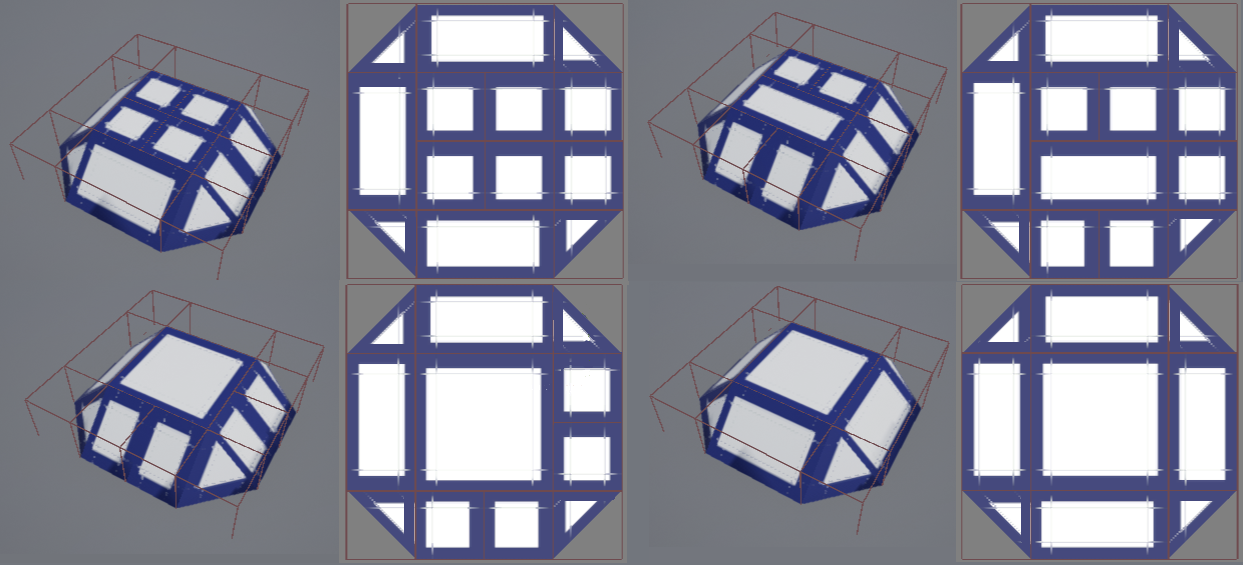
\includegraphics[ width=140mm]{../img/analysis/konfigurace}

\caption{Ekvivalentní konfigurace tvaru. Zdroj: StackOverflow.com~\citep{so_pattern}}
\label{fig:konfig}

\end{figure}

\FloatBarrier

\subsubsection{Komplexní systém rozpoznávání tvarů}
Výše zmíněný přístup k~rozpoznávání tvarů však přináší mnoho nových problémů. Pro příklad uvažme rozklad bloku \RB{A5} netriviální velikosti (kupříkladu [2,~1,~2], tedy šířky jednotkového bloku). Je zřejmé, že stejného tvaru je možné dosáhnout použitím dvou stejných bloků velikosti [1,~1,~1] a~jednoho bloku \RB{A2} velikosti [1,~1,~1] (pokud budeme uvažovat, že je možné tyto dva bloky vzájemně kombinovat). Bloky v~herním světě by se pak musely nějakým způsobem sdružovat do těchto vyšších celků a~ty pak vyhodnocovat vůči definovaným tvarům, či případně jinak rozpoznávat, zda jsou součástí nějakého předem definovaného tvaru. Z~důvodu celkové náročnosti tohoto přístupu jsme se rozhodli, že tento komplexní systém nebudeme v~naší práci požadovat. Nicméně, tato myšlenka se nám velice líbí, takže ji necháme jako možné budoucí rozšíření této práce.






%!TEX root = ../prace.tex

\section{Počasí}

- počasí chceme proměnlivé ale s tím, že gamedesignéři mohou snadno ovlňovat výsledné počasí, případně aby šlo snadno rozšířit varianty pro různé herní módy

-budeme mít ve světě umístenou entitu (Pawn) ovládaný AI Controllerem - to z toho důvodu, že pro AI Controller můžeme použít BehaviorTree

-popsat ideu BT

-další možnosti by byly, že bychom prostě použili update smyčku nějakého Actora - není potřeba, tohle se vyřeší updatem na komponentě

%!TEX root = ../prace.tex

\section{Hráčova postava}

- pohled 1st person, 3rd person

- má komponenty kyslíku, energie

- může stavět, interagovat s bloky

- může zařvat


%!TEX root = ../../prace.tex

\section{Inventář}

Inventář bude vhodné implementovat jako komponentu, kterou posléze můžeme přiřadit herní postavě. Opět se zde opíráme o~fakt, že bychom v~budoucnu mohli mít bloky či \NPC{}, kteří také mají svůj inventář. Z~kapitoly \ref{subsec:inventory} vyplývá, že inventář má několik základních vlastností:

\begin{itemize}
	\item Seznam postavitelných bloků
	\item Seznam umístitelných bloků
	\item Seznam inventárních skupin pro filtrování
\end{itemize}

V momentě, kdy budeme chtít hráči nabídnout bloky k~postavení či umístění, oba seznamy dofiltrujeme dle aktuálně zvolené inventární skupiny. Musíme se tedy zaměřit na to, jak budeme řešit inventární skupiny.

\subsection{Inventární skupiny}

Protože má každý blok své definované \textit{tagy}, musíme vymyslet takový systém, abychom snadno filtrovali podle těchto tagů. Nejsnazší způsob je takový, kdy každá inventární skupina definuje, jaké tagy musí blok mít, aby byl přiřazen. Takže pro blok, který má být zobrazen v~rámci inventární skupiny, platí, že blok definuje všechny tagy v~rámci dané inventární skupiny. Nicméně se může stát, že hráč bude chtít mít v~dané skupině takové bloky, které nemusí splňovat všechny tagy, ale splňují alespoň jeden z~definované skupiny. Z~této myšlenky se dostáváme k~jednoznačnému způsobu filtrování tagů, který je ekvivalentní s~\textit{konjunktivně normální formou} (\CNF{}).


Chceme tedy implementovat takový systém, kdy \textit{inventární skupina} definuje \textit{inventární skupiny tagů} (konjunktivní vyhodnocení), přičemž \textit{inventární skupiny tagů} definují \textit{skupiny tagů} (disjunktivní vyhodnocení). Při vyhodnocování \textit{inventární skupiny} budeme sledovat, zda blok splňuje všechny její \textit{inventární skupiny tagů}, přičemž pro každou z~nich budeme zjišťovat, zda blok definuje alespoň jeden tag ze \textit{skupiny tagů}. 

Abychom hráči ještě více zpříjemnili práci s~inventářem, nebudeme požadovat přesnou shodu tagů definovaných blokem a~\textit{skupinou tagů}. Bude nám totiž stačit pouze podmínka podřetězce, tedy podmínka, aby tag bloku obsahoval jako podřetězec tag ze \textit{skupiny tagů}. Tím dosáhneme toho, že hráč nebude muset v~inventáři vypisovat celé řetězce z~tagů, které si nadefinoval u~svých bloků. 





%!TEX root = ../../prace.tex

\section{Ukládání hry}

- vše se musí korektně uložit

- ?? specifikace binárního formátu zde, nebo v programátorský?

%!TEX root = ../prace.tex

\section{Doplňující vlastnosti}

\subsection{DLC}

- můžeme dodávat extra bloky (ukázka!)

\subsection{Lokalizace}

- použití lokalizace 

\subsection{Hudba}

- atmosférický hudební doprovod




\section{Backlog}

\begin{itemize}
	
	\item Popsat, že bychom chtěli nějaké UI + nabídky menu

\end{itemize}

%%% Fiktivní kapitola s ukázkami tabulek, obrázků a kódu


%!TEX root = ../prace.tex

\chapter{Programátorská dokumentace}

Používání tabulek a grafů v~odborném textu má některá společná
pravidla a~některá specifická. Tabulky a grafy neuvádíme přímo do
textu, ale umístíme je buď na samostatné stránky nebo na vyhrazené
místo v~horní nebo dolní části běžných stránek. \LaTeX\ se o~umístění
plovoucích grafů a tabulek postará automaticky.

Každý graf a tabulku
očíslujeme a umístíme pod ně legendu. Legenda má popisovat obsah grafu
či tabulky tak podrobně, aby jim čtenář rozuměl bez důkladného
studování textu práce.

Na každou tabulku a graf musí být v~textu odkaz
pomocí jejich čísla. Na příslušném místě textu pak shrneme ty
nejdůležitější závěry, které lze z~tabulky či grafu učinit. Text by
měl být čitelný a srozumitelný i~bez prohlížení tabulek a grafů a
tabulky a grafy by měly být srozumitelné i~bez podrobné četby textu.

Na tabulky a grafy odkazujeme pokud možno nepřímo v~průběhu běžného
toku textu; místo \emph{\uv{Tabulka~\ref{tab03:Nejaka} ukazuje, že
    muži jsou v~průměru o~$9,9\,\rm kg$ těžší než ženy}} raději napíšeme
\emph{\uv{Muži jsou o~$9,9\,\rm kg$ těžší než ženy (viz
    Tabulka~\ref{tab03:Nejaka})}}.

\section{Tabulky}

\begin{table}[b!]

\centering
%%% Tabulka používá následující balíčky:
%%%   - booktabs (\toprule, \midrule, \bottomrule)
%%%   - dcolumn (typ sloupce D: vycentrovaná čísla zarovnaná na
%%%     desetinnou čárku
%%%     Všimněte si, že ve zdrojovém kódu jsou desetinné tečky, ale
%%%     tisknou se čárky.
%%% Dále používáme příkazy \pulrad a \mc definované v makra.tex

\begin{tabular}{l@{\hspace{1.5cm}}D{.}{,}{3.2}D{.}{,}{1.2}D{.}{,}{2.3}}
\toprule
 & \mc{} & \mc{\textbf{Směrod.}} & \mc{} \\
\pulrad{\textbf{Efekt}} & \mc{\pulrad{\textbf{Odhad}}} & \mc{\textbf{chyba}$^a$} &
\mc{\pulrad{\textbf{P-hodnota}}} \\
\midrule
Abs. člen     & -10.01 & 1.01 & \mc{---} \\
Pohlaví (muž) & 9.89   & 5.98 & 0.098 \\
Výška (cm)    & 0.78   & 0.12 & <0.001 \\
\bottomrule
\multicolumn{4}{l}{\footnotesize \textit{Pozn:}
$^a$ Směrodatná chyba odhadu metodou Monte Carlo.}
\end{tabular}

\caption{Maximálně věrohodné odhady v~modelu M.}\label{tab03:Nejaka}

\end{table}

U~\textbf{tabulek} se doporučuje dodržovat následující pravidla:

\begin{itemize} %% nebo compactitem z balíku paralist
\item Vyhýbat se svislým linkám. Silnějšími vodorovnými linkami
  oddělit tabulku od okolního textu včetně legendy, slabšími
  vodorovnými linkami oddělovat záhlaví sloupců od těla tabulky a
  jednotlivé části tabulky mezi sebou. V~\LaTeX u tuto podobu tabulek
  implementuje balík \texttt{booktabs}. Chceme-li výrazněji oddělit
  některé sloupce od jiných, vložíme mezi ně větší mezeru.
\item Neměnit typ, formát a význam obsahu políček v~tomtéž sloupci
  (není dobré do téhož sloupce zapisovat tu průměr, onde procenta).
\item Neopakovat tentýž obsah políček mnohokrát za sebou. Máme-li
  sloupec \textit{Rozptyl}, který v~prvních deseti řádcích obsahuje
  hodnotu $0,5$ a v~druhých deseti řádcích hodnotu $1,5$, pak tento
  sloupec raději zrušíme a vyřešíme to jinak. Například můžeme tabulku
  rozdělit na dvě nebo do ní vložit popisné řádky, které informují
o~nějaké proměnné hodnotě opakující se v~následujícím oddíle tabulky
  (např. \emph{\uv{Rozptyl${}=0,5$}} a níže \emph{\uv{Rozptyl${}=
      1,5$}}).
\item Čísla v~tabulce zarovnávat na desetinnou čárku.
\item V~tabulce je někdy potřebné používat zkratky, které se jinde
nevyskytují. Tyto zkratky můžeme vysvětlit v~legendě nebo
v~poznámkách pod tabulkou. Poznámky pod tabulkou můžeme využít i
k~podrobnějšímu vysvětlení významu  některých sloupců nebo hodnot.
\end{itemize}

\section{Obrázky}

Několik rad týkajících se obrázků a grafů.

\begin{itemize}
\item Graf by měl být vytvořen ve velikosti, v~níž bude použit
  v~práci. Zmenšení příliš velkého grafu vede ke špatné čitelnosti
  popisků.
\item Osy grafu musí být řádně popsány ve stejném jazyce, v~jakém je
  psána práce (absenci diakritiky lze tolerovat). Kreslíme-li graf
  hmotnosti proti výšce, nenecháme na nich popisky \texttt{ht} a
  \texttt{wt}, ale osy popíšeme \emph{Výška [cm]} a~\emph{Hmotnost
    [kg]}. Kreslíme-li graf funkce $h(x)$, popíšeme osy $x$ a $h(x)$.
  Každá osa musí mít jasně určenou škálu.
\item Chceme-li na dvourozměrném grafu vyznačit velké množství bodů,
  dáme pozor, aby se neslily do jednolité černé tmy. Je-li bodů mnoho,
  zmenšíme velikost symbolu, kterým je vykreslujeme, anebo vybereme
  jen malou část bodů, kterou do grafu zaneseme. Grafy, které obsahují
  tisíce bodů, dělají problémy hlavně v~elektronických dokumentech,
  protože výrazně zvětšují velikost souborů.
\item Budeme-li práci tisknout černobíle, vyhneme se používání barev.
  Čáry roz\-li\-šu\-je\-me typem (plná, tečkovaná, čerchovaná,\ldots), plochy
  dostatečně roz\-díl\-ný\-mi intensitami šedé nebo šrafováním. Význam
  jednotlivých typů čar a~ploch vysvětlíme buď v~textové legendě ke
  grafu anebo v~grafické legendě, která je přímo součástí obrázku.
\item Vyhýbejte se bitmapovým obrázkům o~nízkém rozlišení a zejména
  JPEGům (zuby a kompresní artefakty nevypadají na papíře pěkně).
  Lepší je vytvářet obrázky vektorově a vložit do textu jako PDF.
\end{itemize}

\section{Programy}

Algoritmy, výpisy programů a popis interakce s~programy je vhodné
odlišit od ostatního textu. Jednou z~možností je použití {\LaTeX}o\-vé\-ho balíčku
\texttt{fancyvrb} (fancy verbatim), pomocí něhož je v~souboru \texttt{makra.tex}
nadefinováno prostředí \texttt{code}. Pomocí něho lze vytvořit
např. následující ukázky.

\begin{code}
> mean(x)
[1] 158.90
> objekt$prumer
[1] 158.90
\end{code}
%$
Menší písmo:
\begin{code}[fontsize=\footnotesize]
> mean(x)
[1] 158.90
> objekt$prumer
[1] 158.90
\end{code}
%$
Bez rámečku:
\begin{code}[frame=none]
> mean(x)
[1] 158.90
> objekt$prumer
[1] 158.90
\end{code}
%$
Užší rámeček:
\begin{code}[xrightmargin=20em]
> mean(x)
[1] 158.90
> objekt$prumer
[1] 158.90
\end{code}
%$

\begin{figure}[p]\centering
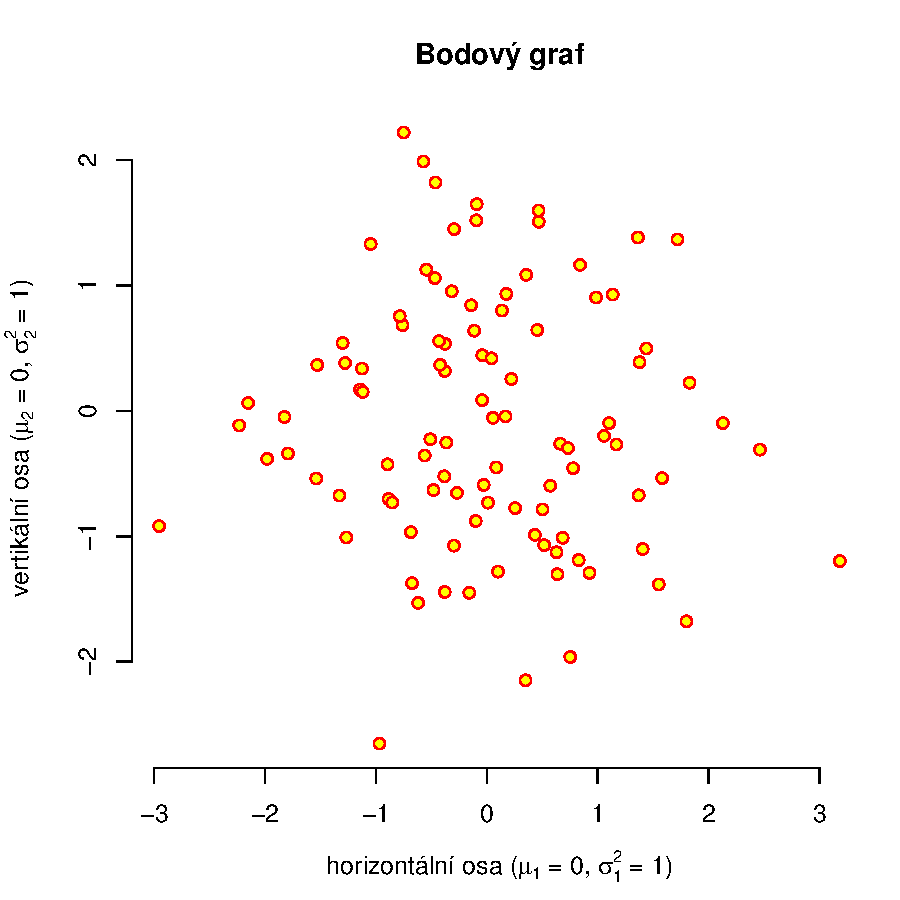
\includegraphics[width=140mm, height=140mm]{../img/ukazka-obr01}
% Příponu není potřeba explicitně uvádět, pdflatex automaticky hledá pdf.
% Rozměry také není nutné uvádět.
\caption{Náhodný výběr z~rozdělení $\mathcal{N}_2(\boldsymbol{0},\,I)$.}
\label{obr03:Nvyber}

\end{figure}

\begin{figure}[p]\centering
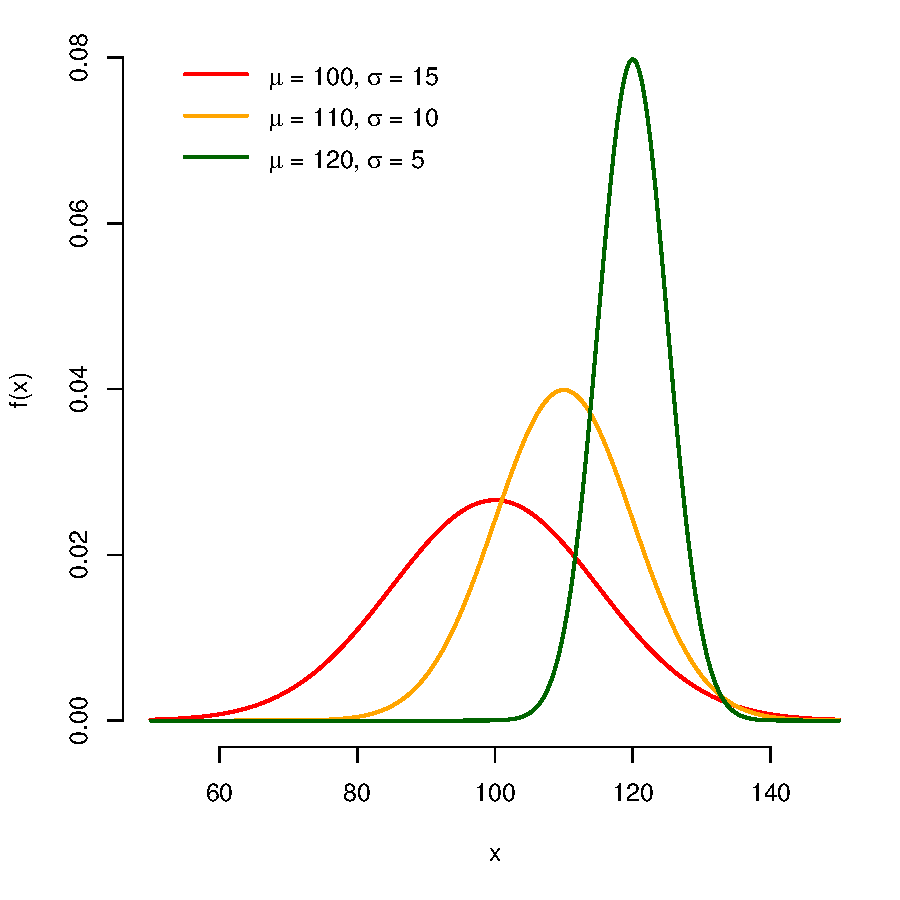
\includegraphics[width=140mm, height=140mm]{../img/ukazka-obr02}
\caption{Hustoty několika normálních rozdělení.}
\label{obr03:Nhust}
\end{figure}

\begin{figure}[p]\centering
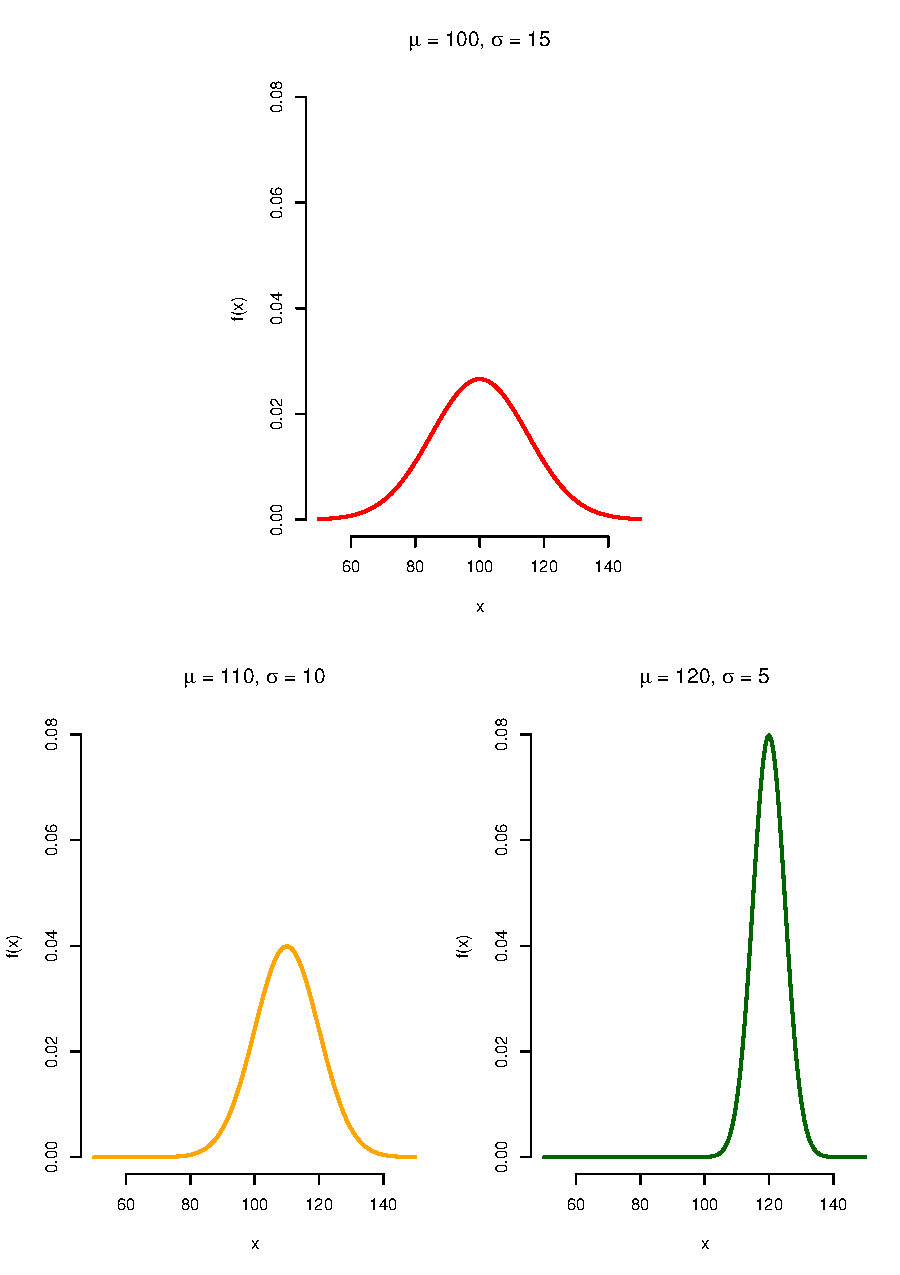
\includegraphics[width=140mm, height=198mm]{../img/ukazka-obr03}
\caption{Hustoty několika normálních rozdělení.}
\label{obr03:Nhust:podruhe}

\end{figure}

%!TEX root = ../prace.tex

\chapter{Uživatelská dokumentace}

\section{Požadavky pro spuštění hry}
\subsubsection{Hardwarové požadavky}

Doporučená minimální sestava (na ní byla hra vyvíjena): 

\begin{center}
	\begin{tabular} { | l | l |}
		\hline
		Procesor: 	&	Intel i7-2630QM @ 2.00GHz \\	\hline
		RAM:		&	12 GB	(8 GB by mělo také stačit) \\	\hline
		Grafika:	&	ATI Radeon HD 6700M \\	\hline
		OS:			&	Win 10 x64	(7 a~vyšší by měly též fungovat) \\
		\hline
	\end{tabular}
\end{center}

Výše uvedneou konfiguraci je potřeba brát jako orientační. Hru jsme úspěšně spustili i~na notebooku s~procesorem Intel i5, integrovanou grafickou kartou a~8 GB operační paměti. Bylo však nutné nastavit grafické vlastnosti na minimální možnou konfiguraci. 

\subsubsection{Softwarové požadavky}

Pro spuštění zkompilované hry není potřeba nic speciálního. Je zapotřebí mít stroj s~minimální uvedenou konfigurací. Dále je dobré mít nainstalované poslední verze ovladačů HW komponent (hlavně grafiky). Taktéž je zapotřebí mít nainstalovanou poslední verzi DirectX a~C++ runtime. Tyto části lze doinstalovat z~přiloženého DVD ze složky \textit{Redist}.


\section{Tutoriál}
Tato hra obsahuje pokročilý tutoriál, ve kterém se lze snadno naučit veškeré principy hry. Ten je dostupný z~dialogu výběru nové hry. Proto se nebudeme zabývat podrobným popisem uživatelské dokumentace.
\begin{figure}[!ht]\centering
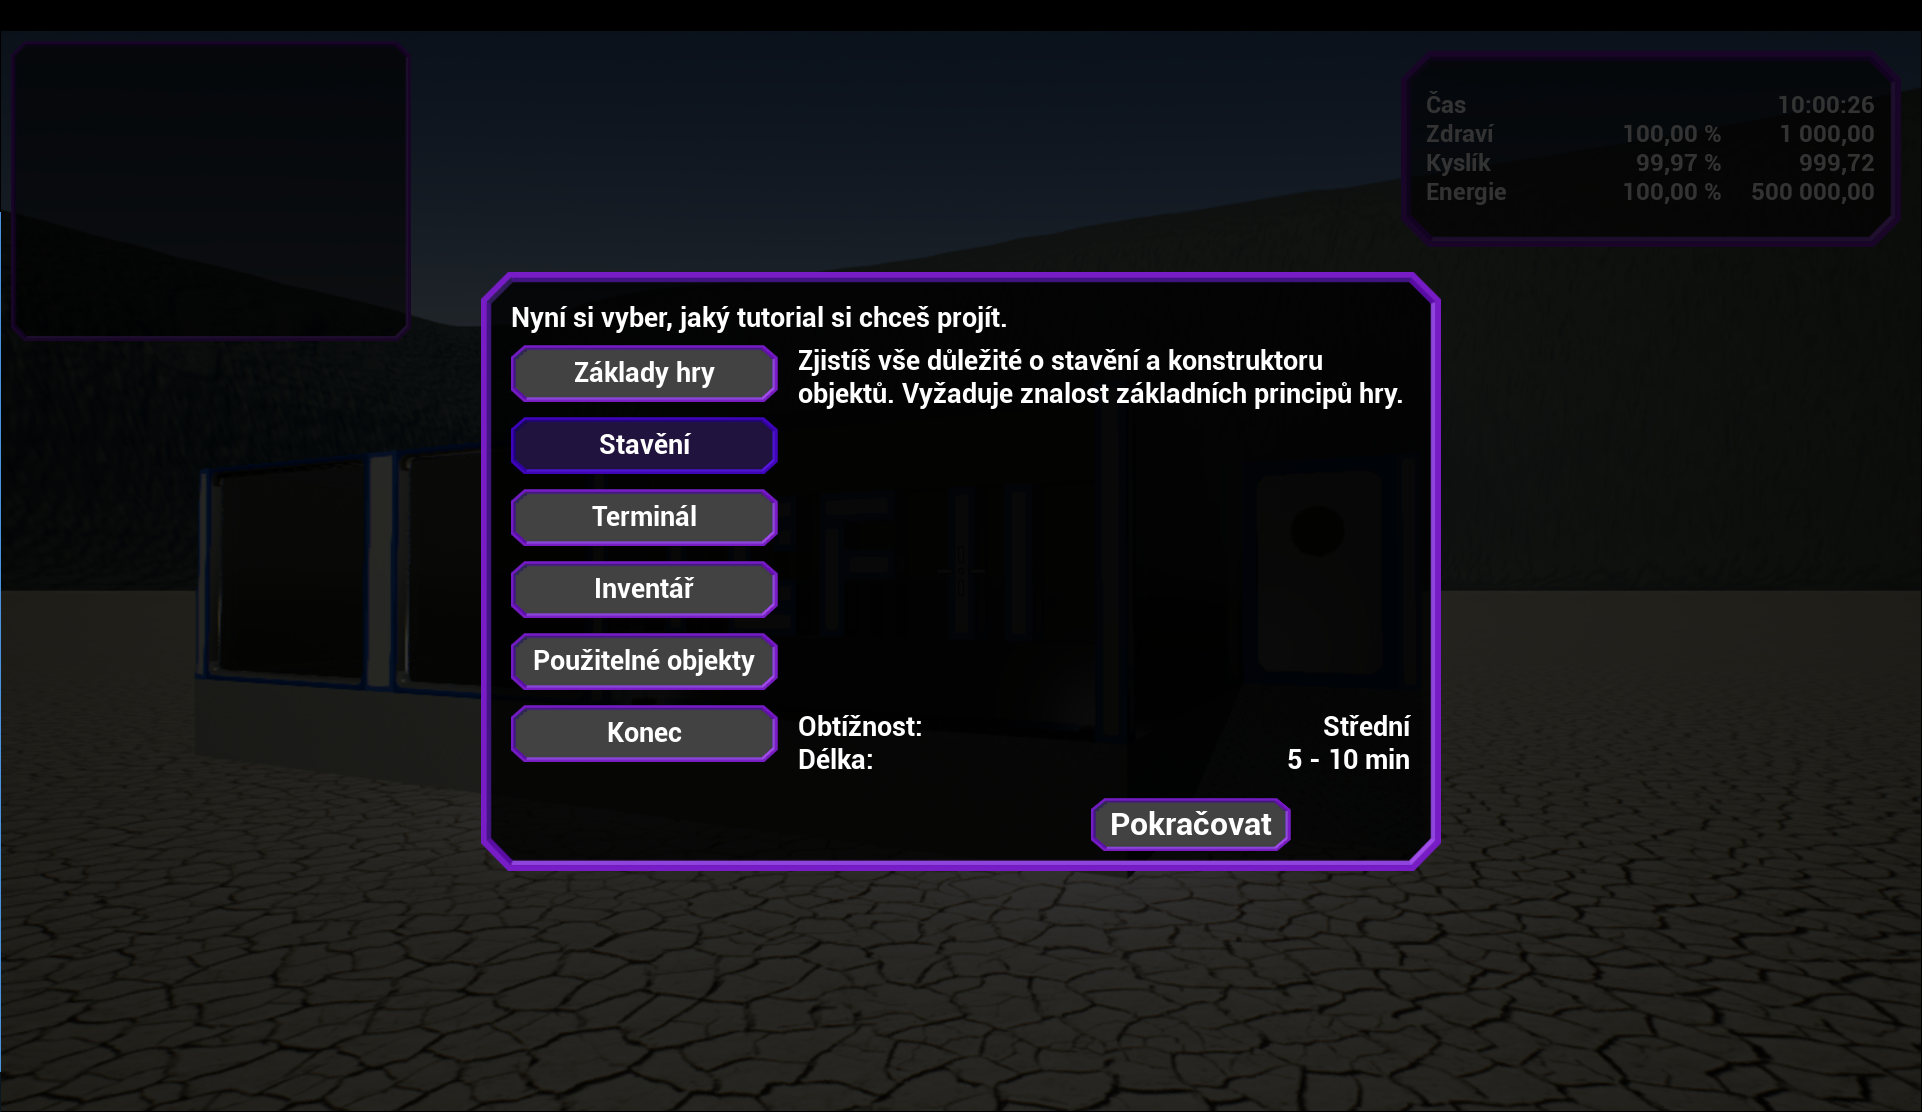
\includegraphics[ width=140mm]{../img/user/mainMenu/mmTut}

\caption{Výběr herního tutoriálu}
\label{fig:usr_tut}

\end{figure}
\FloatBarrier


%!TEX root = ../../prace.tex

\section{Hlavní menu}

Po načtení hry hráč vidí hlavní menu. Denní doba i~počasí se zvolí náhodně.

\begin{figure}[!ht]\centering
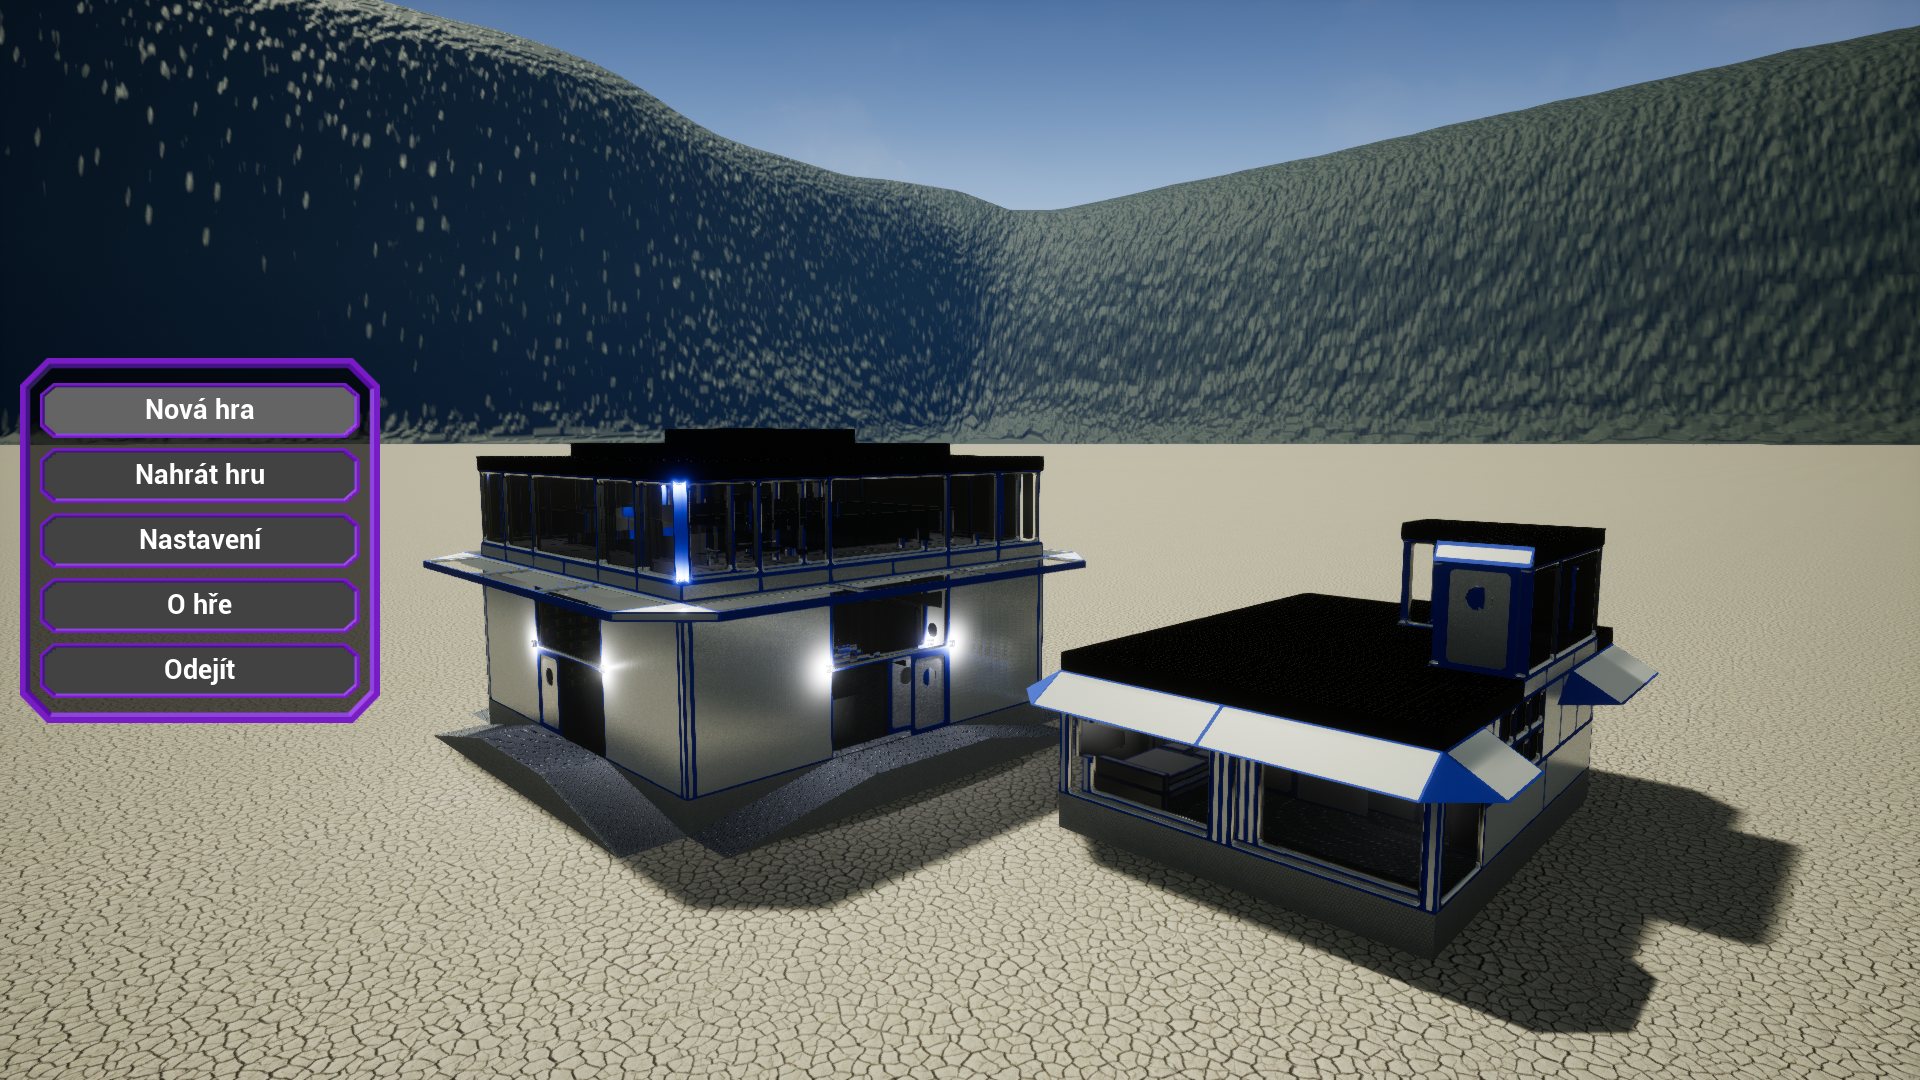
\includegraphics[ width=140mm]{../img/user/mainMenu/mmDay}

\caption{Obrazovka hlavního menu -- den}
\label{fig:user_mainMenu_mmDay}

\end{figure}


\FloatBarrier

První volba, kterou je možné zvolit, je výběr nové hry. K~dispozici je několik variant s~různými obtížnostmi.

\begin{figure}[!ht]\centering
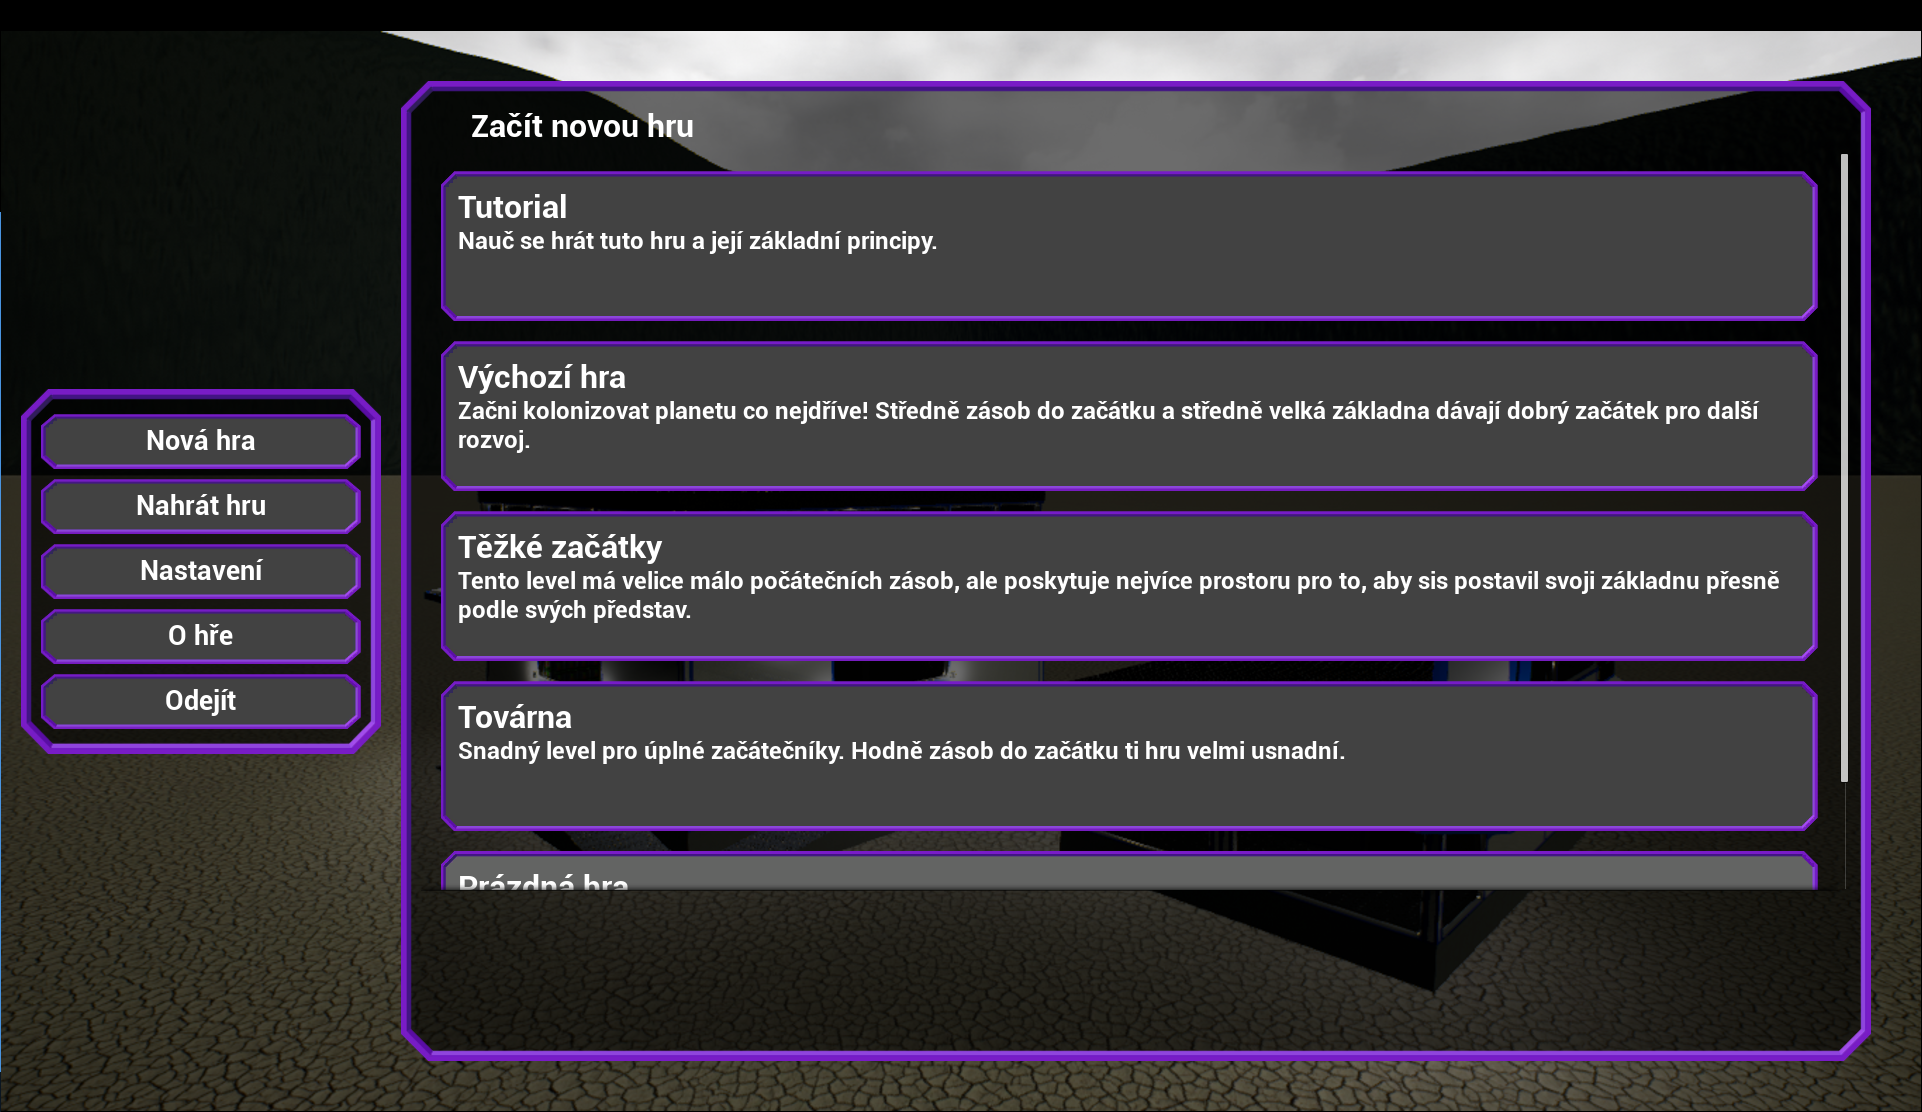
\includegraphics[ width=140mm]{../img/user/mainMenu/mmBegin}

\caption{Obrazovka hlavního menu -- Nová hra}
\label{fig:user_mainMenu_mmBegin}

\end{figure}
\FloatBarrier

Pokud hráč má nějaké uložené hry, může si je nahrát kliknutím na tlačítko \textbf{Nahrát hru}. V~tomto případě žádné uložené hry k~načtení k~dispozici nejsou.

\begin{figure}[!ht]\centering
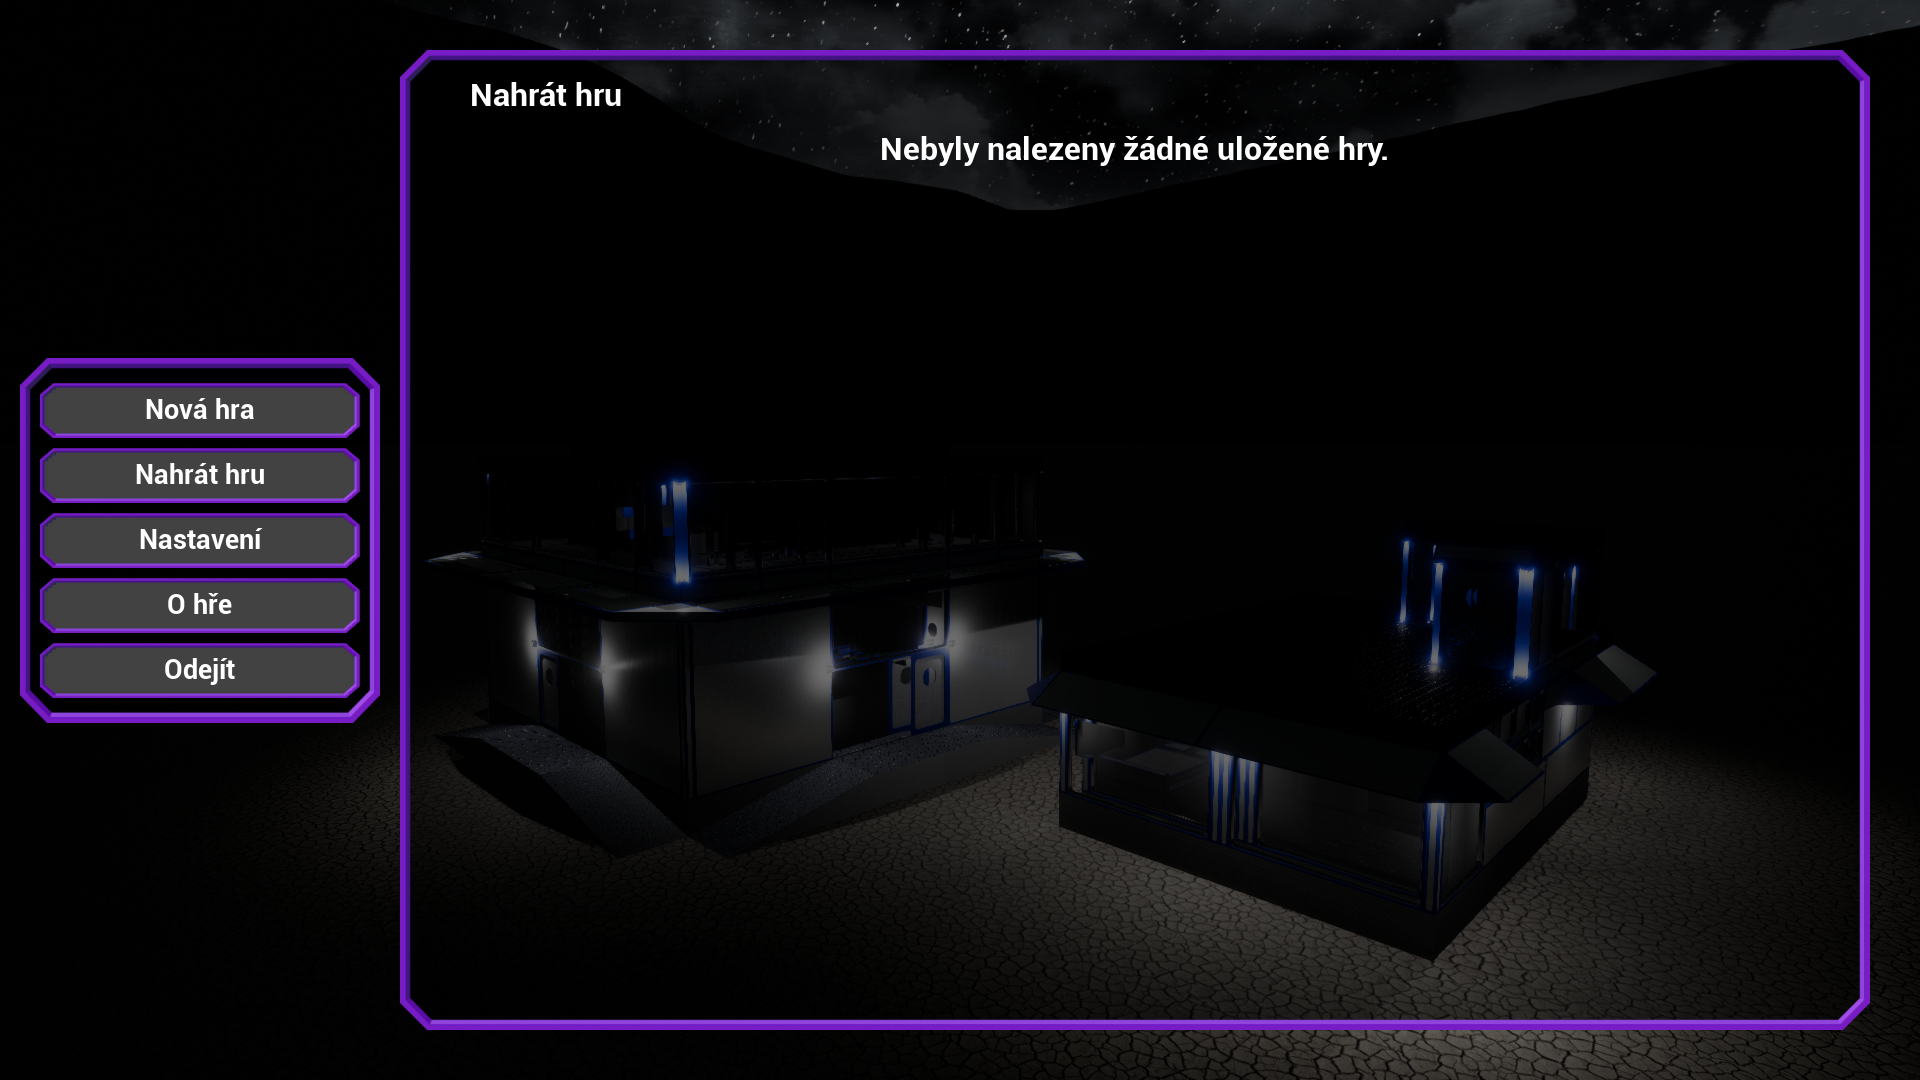
\includegraphics[ width=140mm]{../img/user/mainMenu/mmLoad}

\caption{Obrazovka hlavního menu -- Nahrát hru}
\label{fig:user_mainMenu_mmLoad}

\end{figure}
\FloatBarrier

Pod položkou \textbf{Nastavení} může uživatel měnit herní, zvuková a~grafická nastavení hry. Nastavení se aplikují a~ukládají okamžitě, výjimkou je pouze položka \textit{Animace generátoru energie}, která se projeví až po změně levelu. V~případě konfigurace z~hlavní nabídky se nastavení projeví okamžitě, v~případě konfigurace během rozehrané hry je potřeba vyvolat opětovné načtení uložené hry, nebo znovu spustit novou hru.

\begin{figure}[!ht]\centering
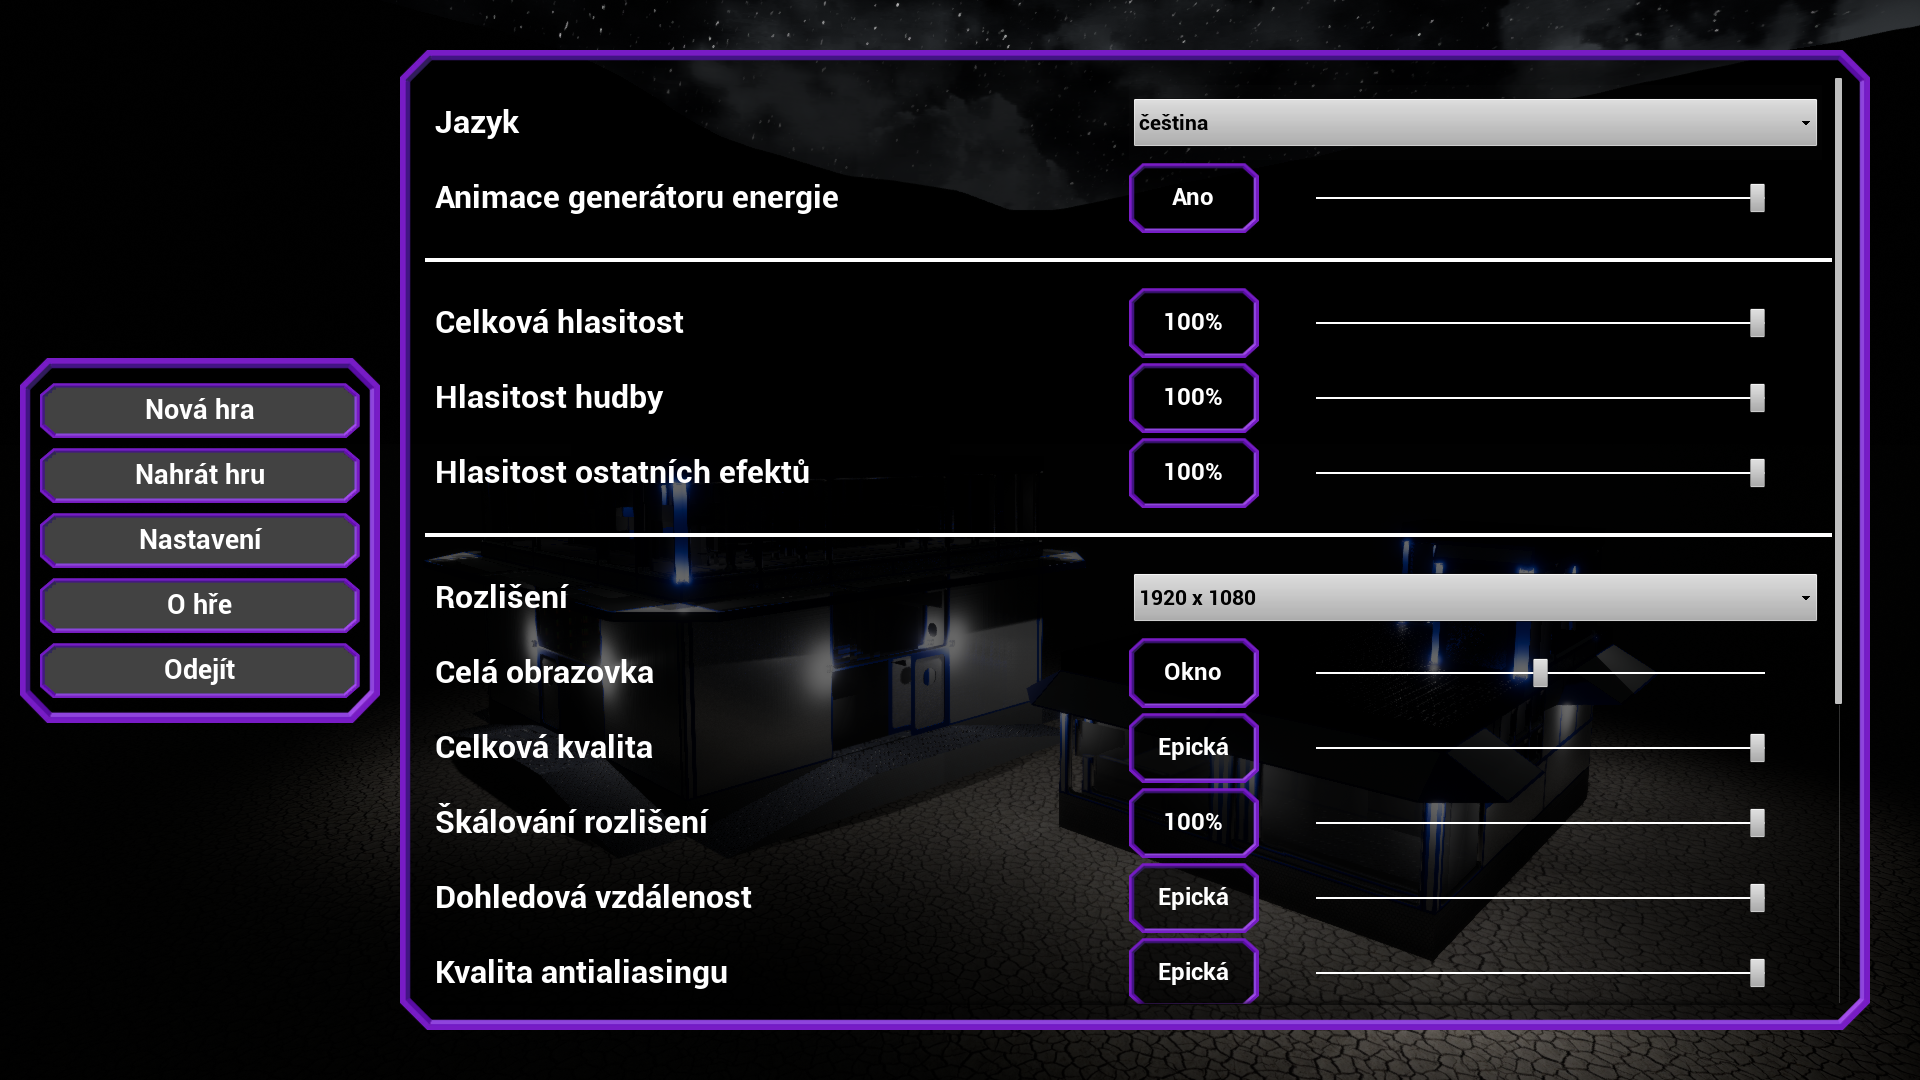
\includegraphics[ width=140mm]{../img/user/mainMenu/mmSettings}

\caption{Obrazovka hlavního menu -- Nastavení}
\label{fig:user_mainMenu_mmSettings}

\end{figure}

\FloatBarrier
%!TEX root = ../../prace.tex

\section{Herní menu - ukládání, nahrávání}

V průběhu rozehrané hry je možné použít \textbf{Rychlé uložení / načtení}, nebo si hru uložit z~herní nabídky.

Pro uložení hry je možné vytvořit nový save nebo přepsat stávající, pokud nějaký existuje. Uložené hry je též možné mazat.

\begin{figure}[!ht]\centering
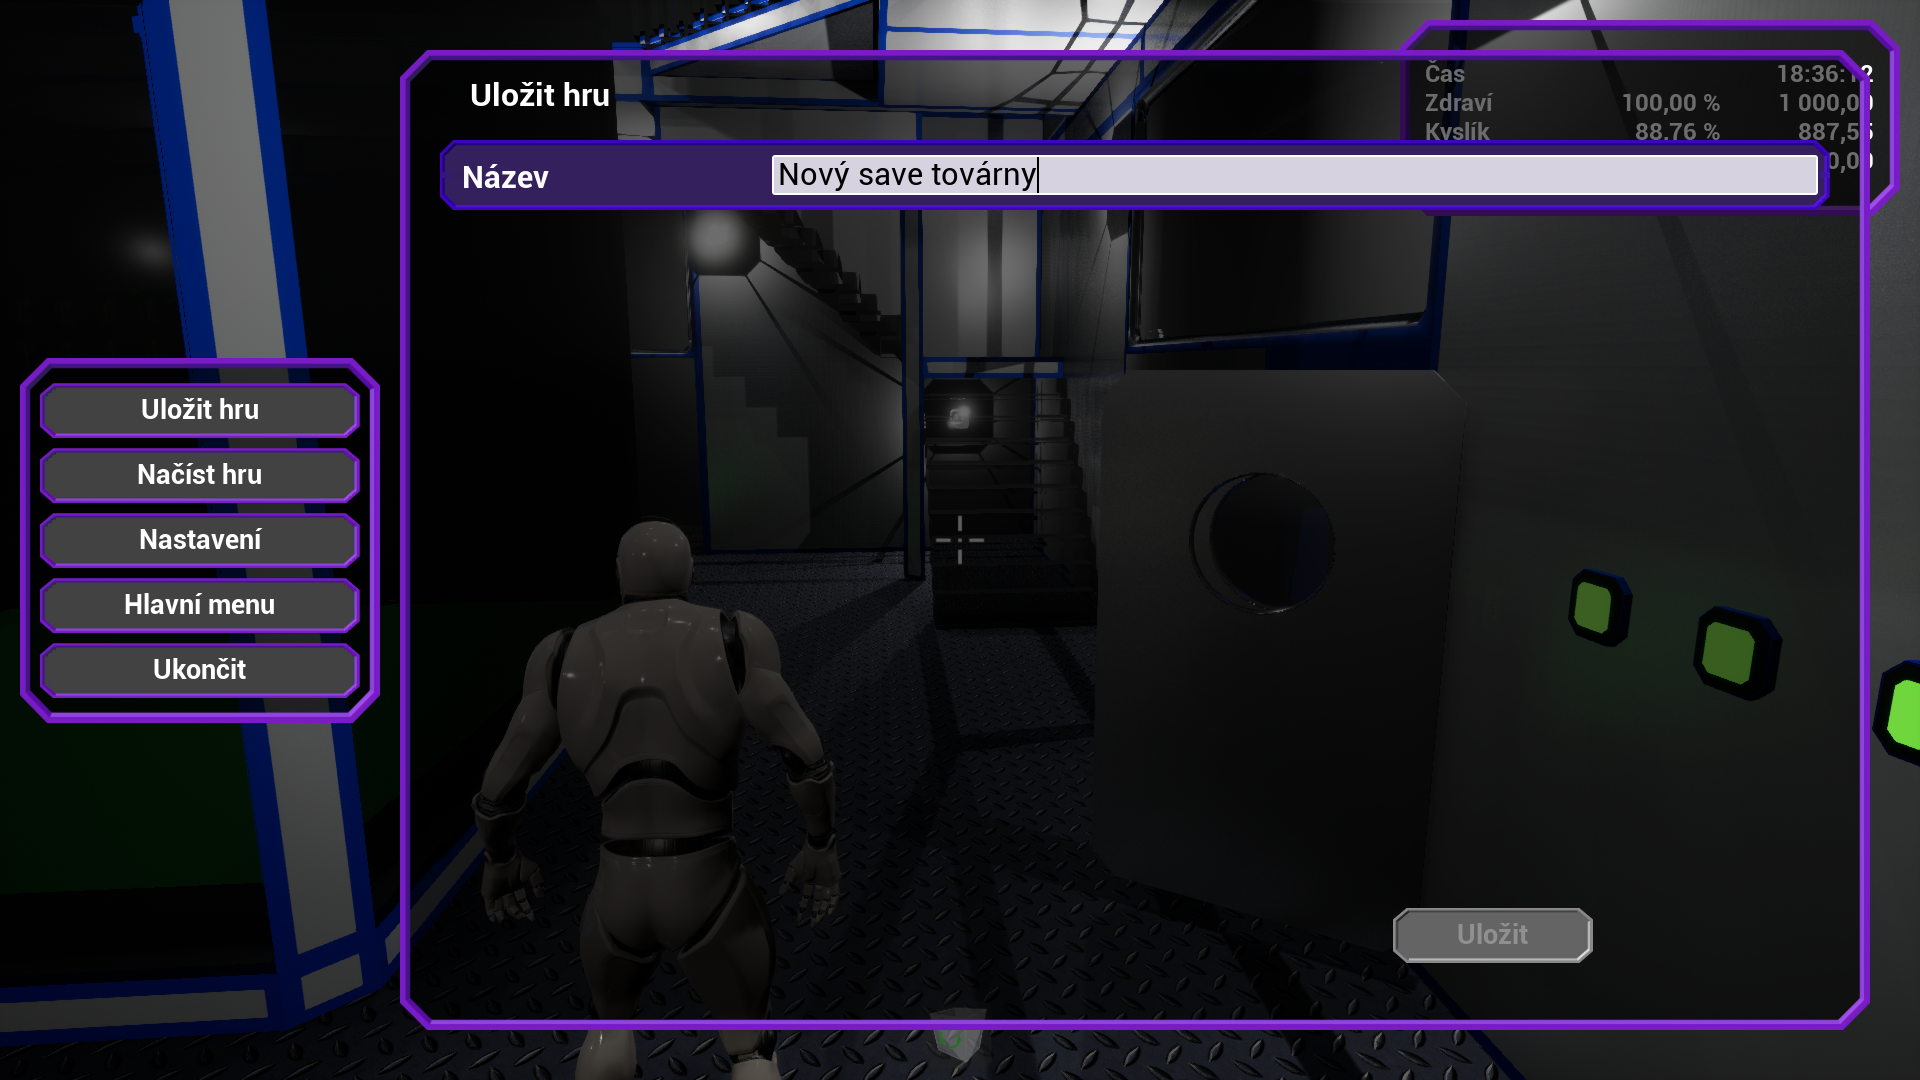
\includegraphics[ width=140mm]{../img/user/save/0newSave}

\caption{Ukládání - Nový save}
\label{fig:user_save_0newSave}

\end{figure}
\FloatBarrier

Pokud bylo uložení úspěšné, hráči se zobrazí následující hláška:

\begin{figure}[!ht]\centering
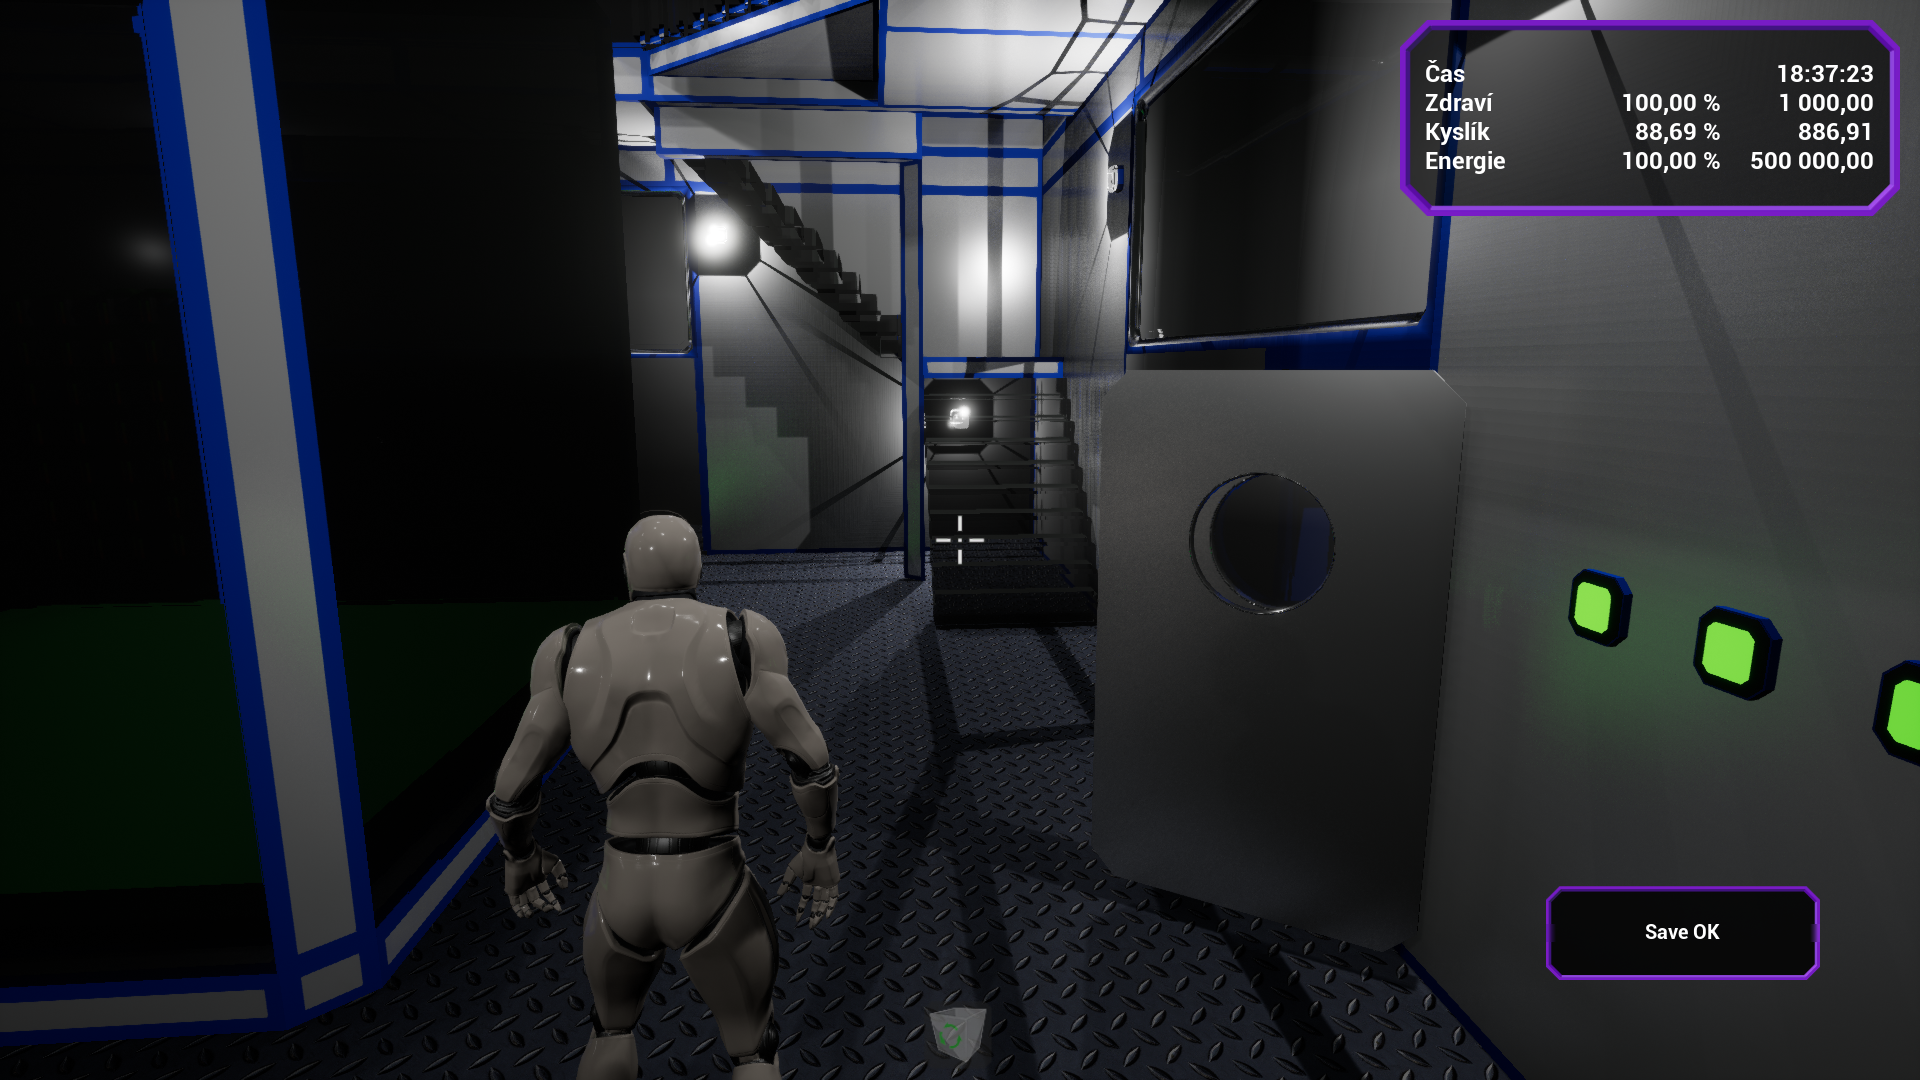
\includegraphics[ width=140mm]{../img/user/save/1afterSave}

\caption{Ukládání - po uložení}
\label{fig:user_save_1afterSave}

\end{figure}
\FloatBarrier

Nahrávat je možné ze všech uložených pozic, včetně rychlého uložení. Opět je zde možné vybraný save smazat.

\begin{figure}[!ht]\centering
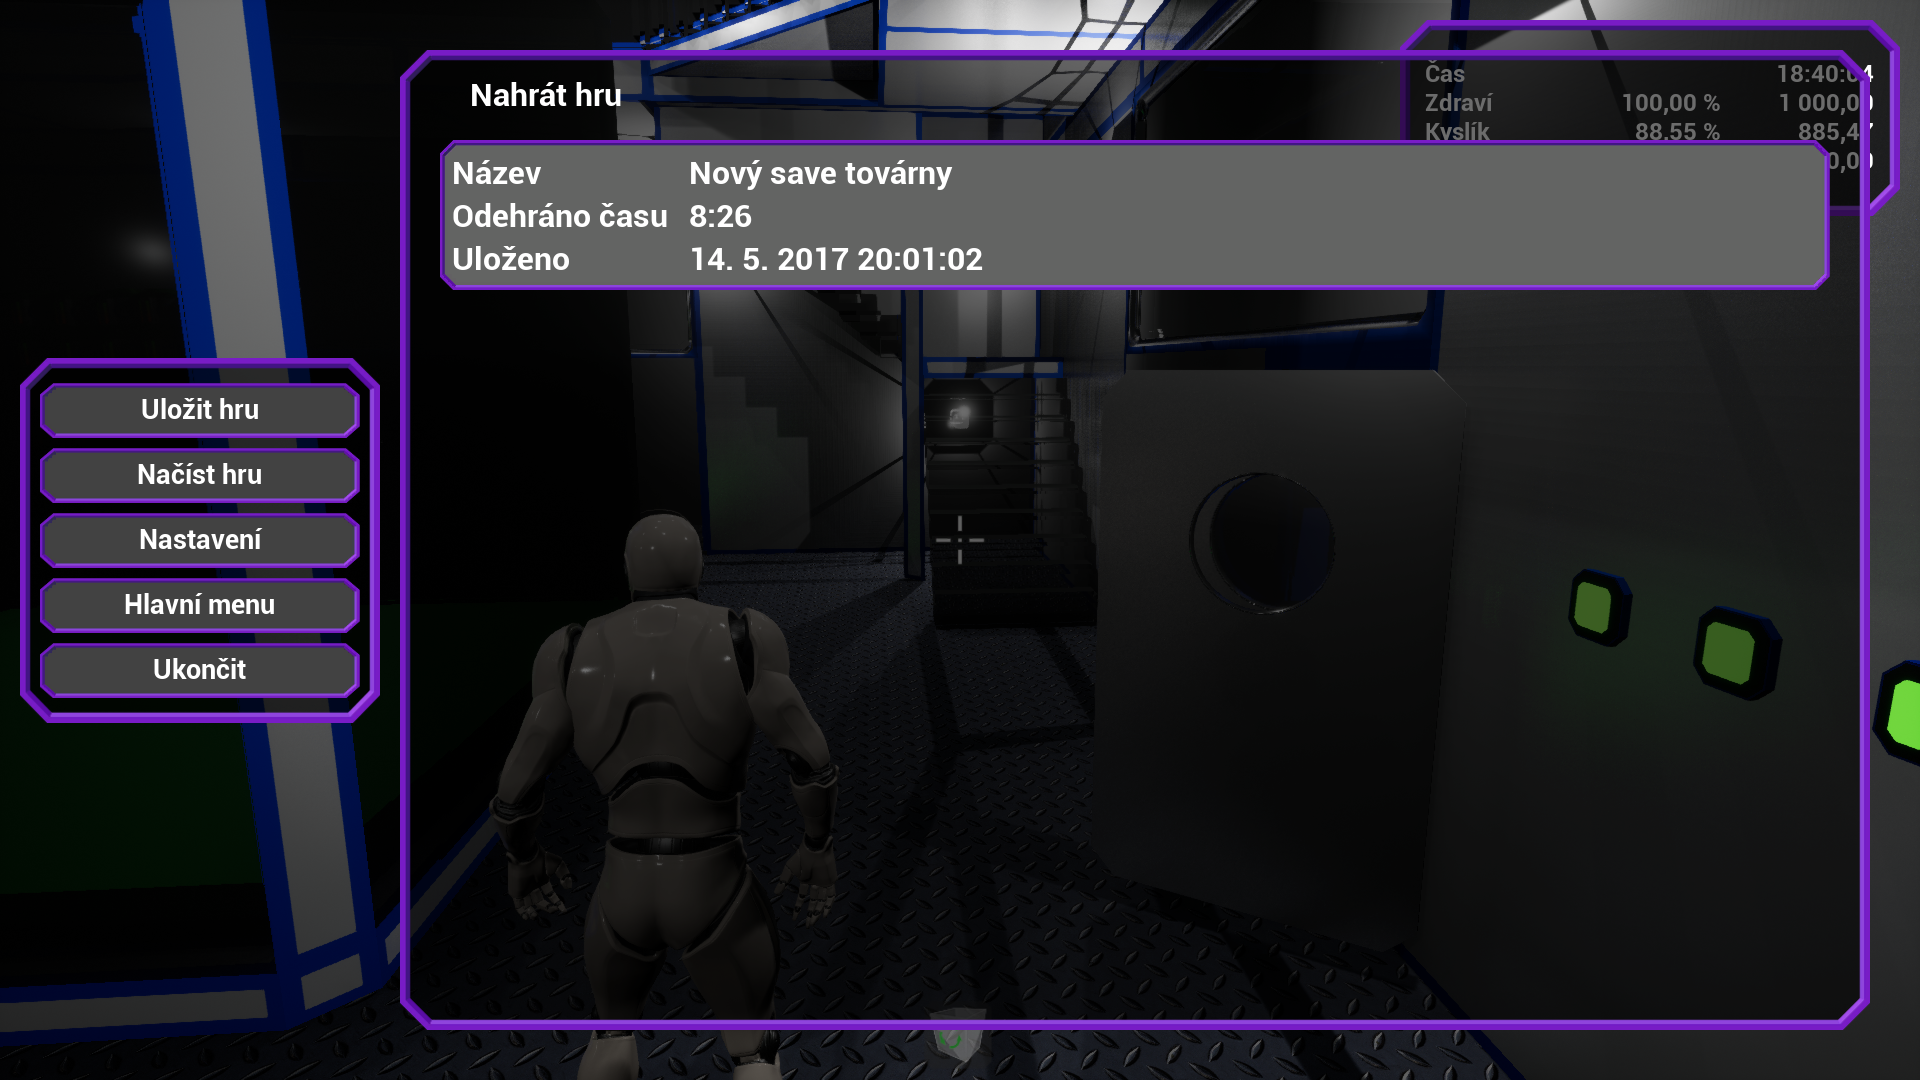
\includegraphics[ width=140mm]{../img/user/save/2load}

\caption{Ukládání - nahrát hru}
\label{fig:user_save_2load}

\end{figure}
\FloatBarrier

Pokud má hráč rozehranou hru, je pro jistotu vyžadováno potvrzení.

\begin{figure}[!ht]\centering
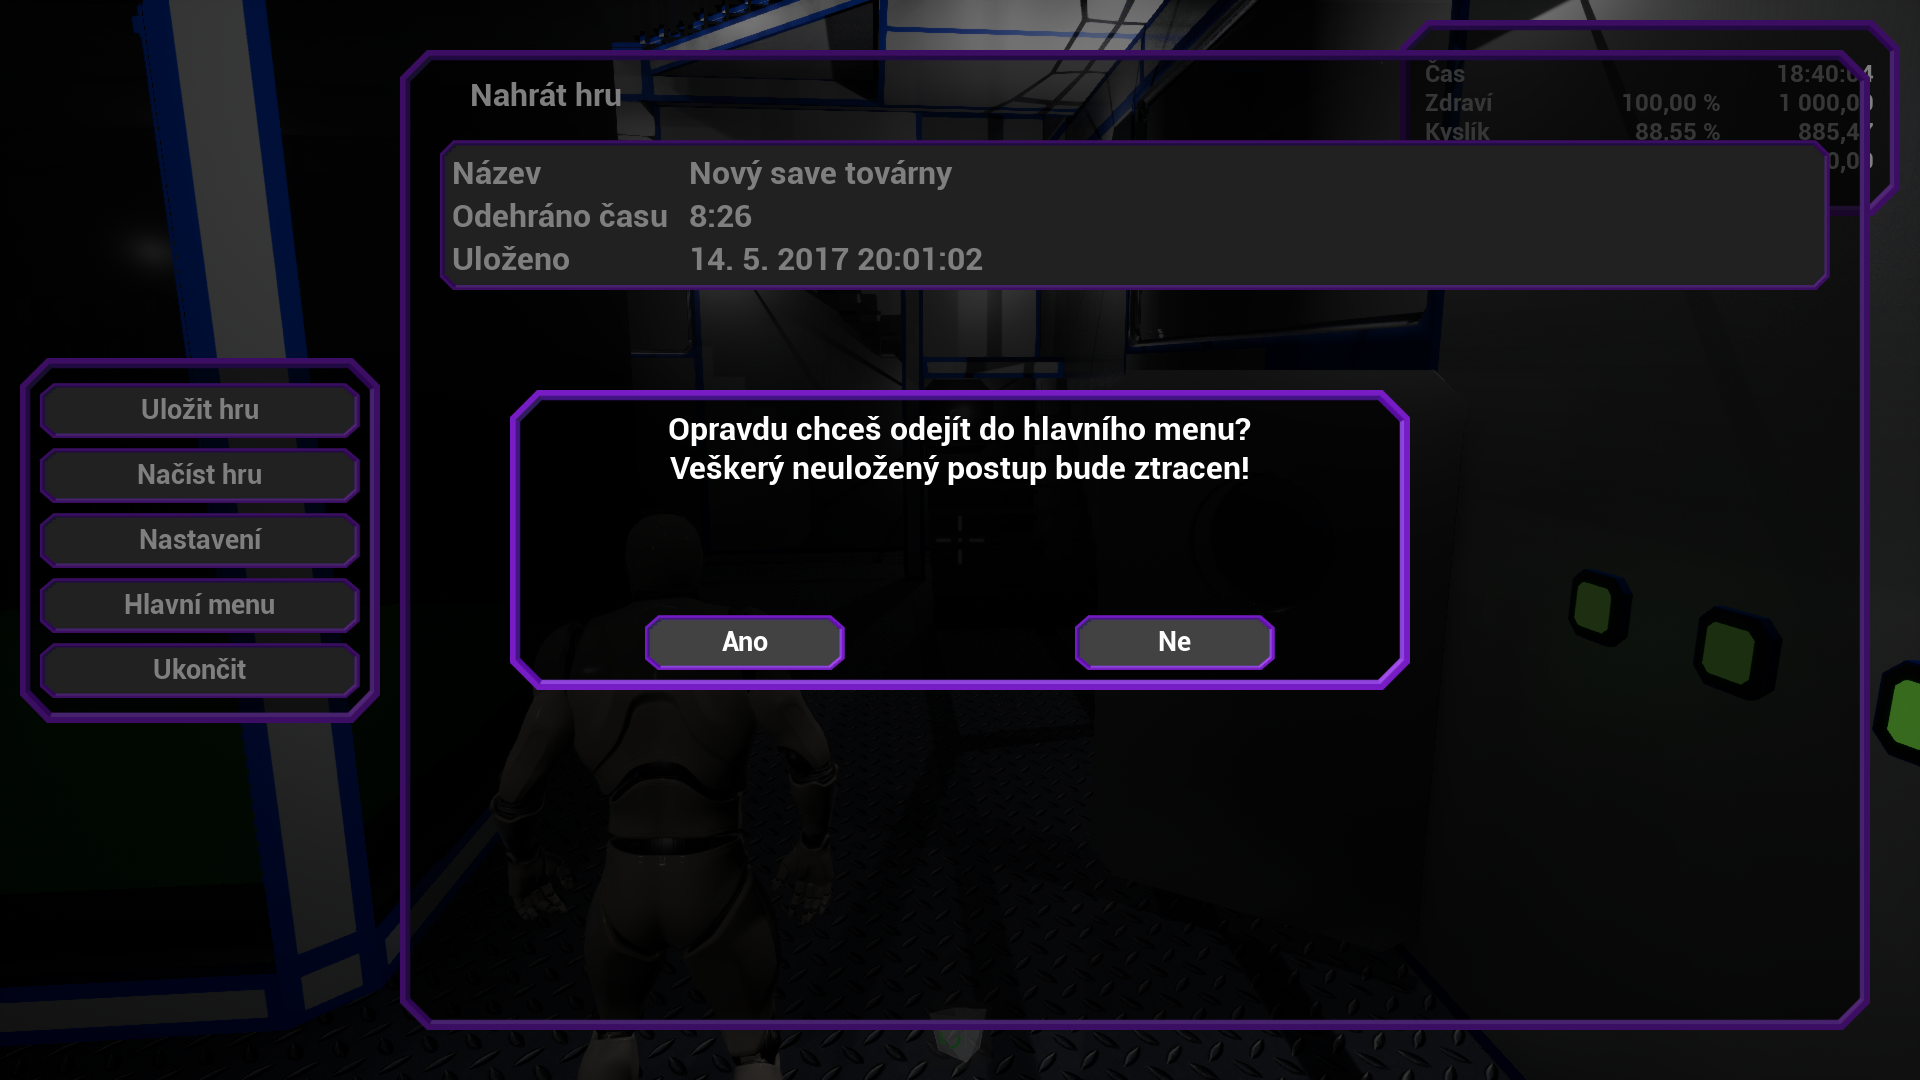
\includegraphics[ width=140mm]{../img/user/save/3loadClicked}

\caption{Ukládání - potvrzení nahrání hry}
\label{fig:user_save_3loadClicked}

\end{figure}

\FloatBarrier
%!TEX root = ../../prace.tex

\section{Inventář}

Inventář se vyvolá klávesou \textbf{E}. Zobrazí se následující obrazovka:

\begin{figure}[!ht]\centering
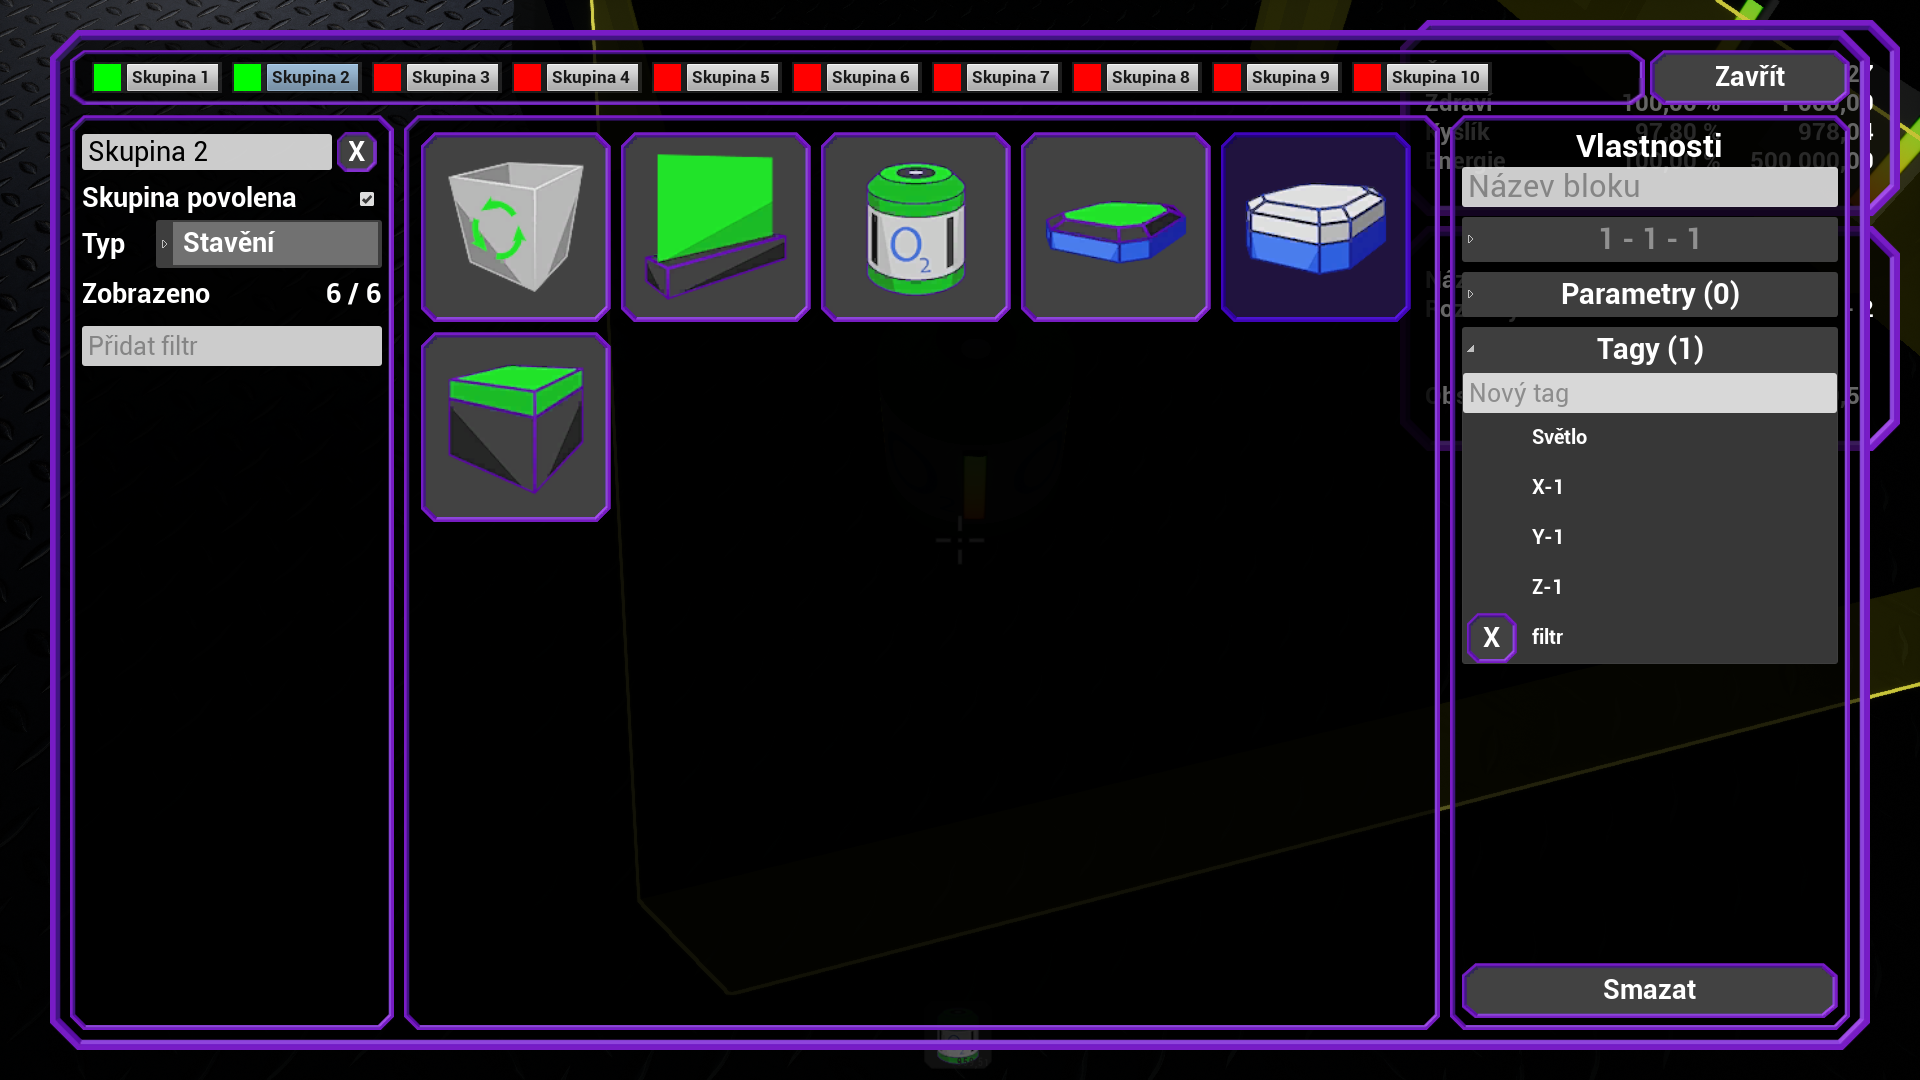
\includegraphics[ width=140mm]{../img/user/inventory/0AddTag}

\caption{Inventář - přehled}
\label{fig:user_inventory_0AddTag}

\end{figure}

\FloatBarrier

V horní části je výběr skupin. Je možné vybírat z 10 skupin, které si lze pojmenovat dle libosti. Dále je možné je (de)aktivovat buď kliknutím na zelený / červený čtverec, nebo skrze příslušný checkbox v editaci skupiny.
Je možné používat standardní změnu skupiny klávesami \textbf{ú} a \textbf{)}, editační okno se pak příslušným způsobem změní. 

V \textit{levé} části je \textbf{editor skupiny}, jehož funkce budou popsány v textu dále. \textit{Uprostřed} je možné vidět postavitelné či umístitelné položky, které jsou dofiltrovány dle právě nastaveného filtru. Výběrem položky lze editovat její vlastnosti v \textit{pravé} části okna

\FloatBarrier

Každá skupina umožňuje definovat své filtry. Matematicky bychom mohli popsat filtrování jako vyhodnocení formule v \textit{CNF}. Pokud do pole \textit{Přidat filtr} napíšeme tagy oddělené mezerou, do skupiny se přidá \textbf{nová} skupina s výchozím pojmenováním.

\begin{figure}[!ht]\centering
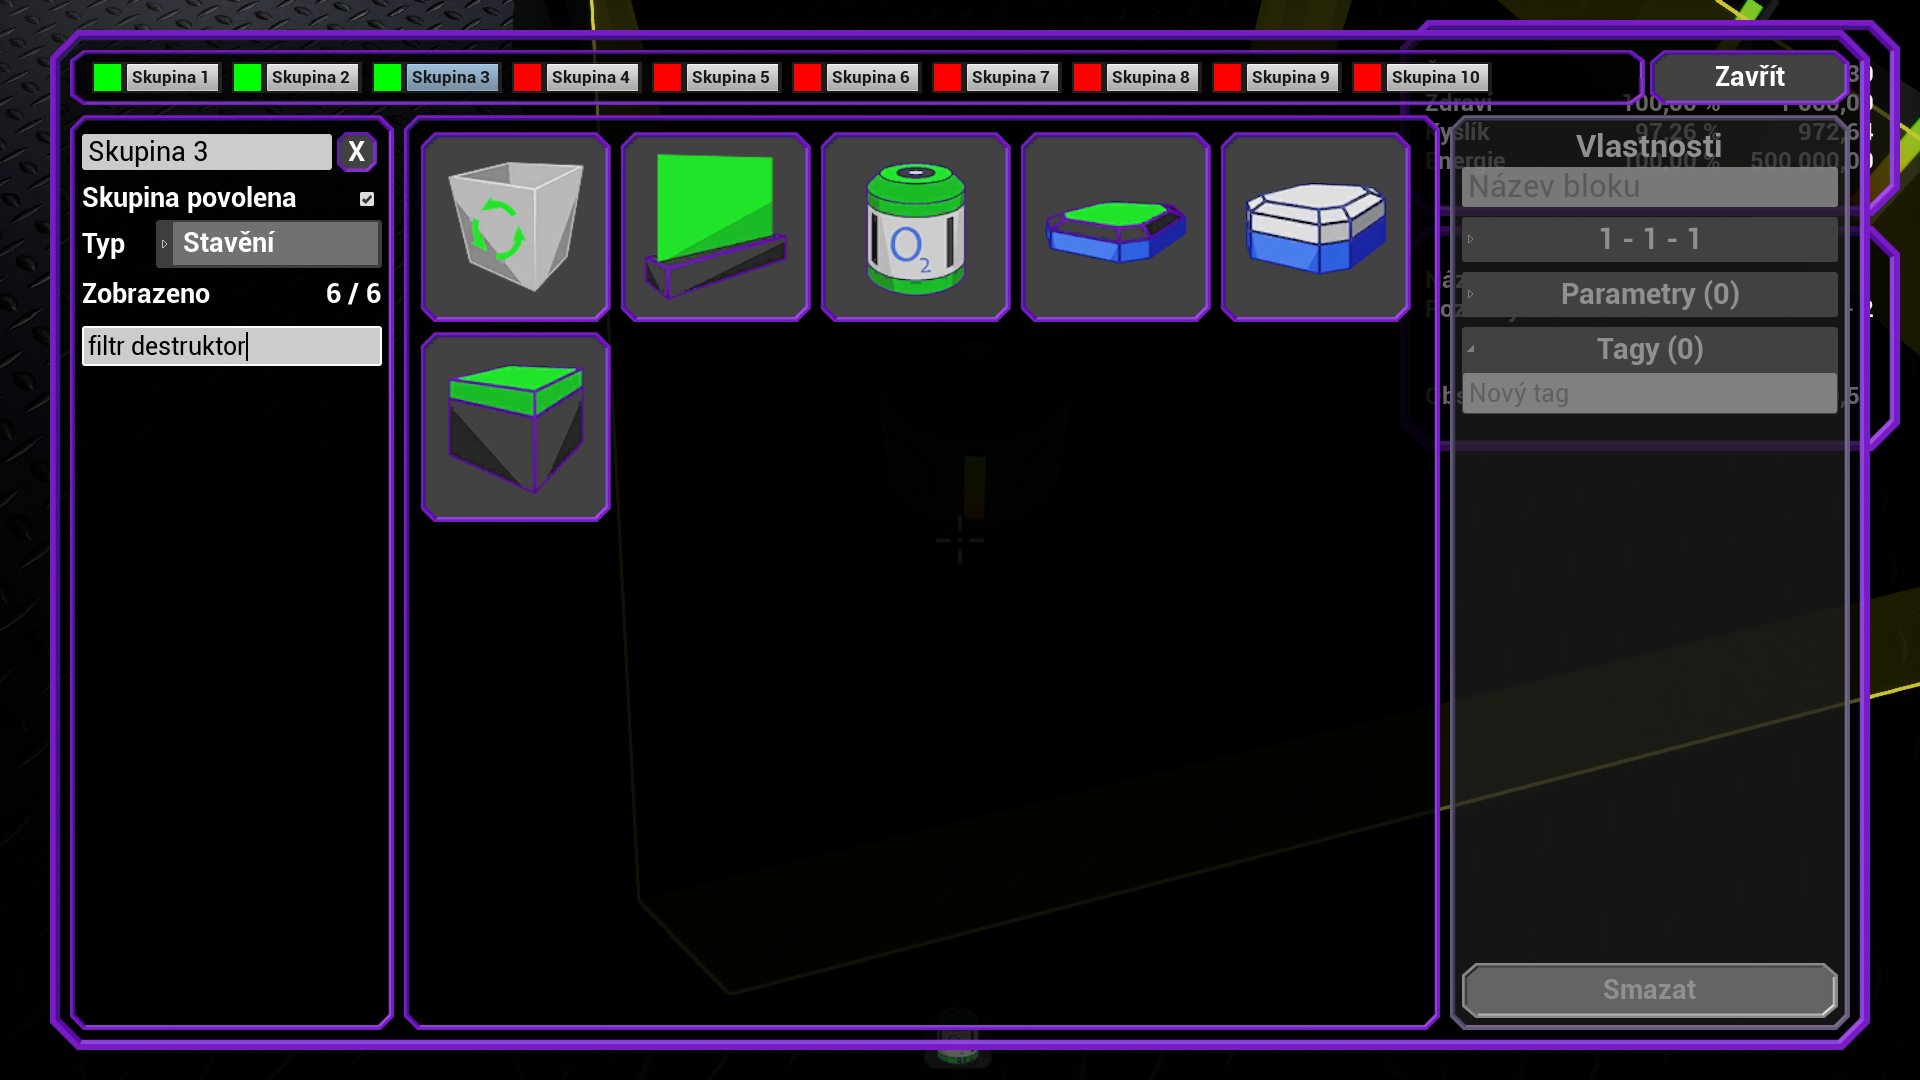
\includegraphics[ width=140mm]{../img/user/inventory/1setFilter}

\caption{Inventář - přidání skupiny}
\label{fig:user_inventory_1setFilter}

\end{figure}

\FloatBarrier

Po přidání se seznam dostupných prvků dofiltruje podle nastavených tagů - ve výsledku bude každá položka splňovat alespoň jeden tag z každé skupiny. Shoda nemusí být přesná, tag objektu musí obsahovat podřetězec definovaný filtrem.
\begin{figure}[!ht]\centering
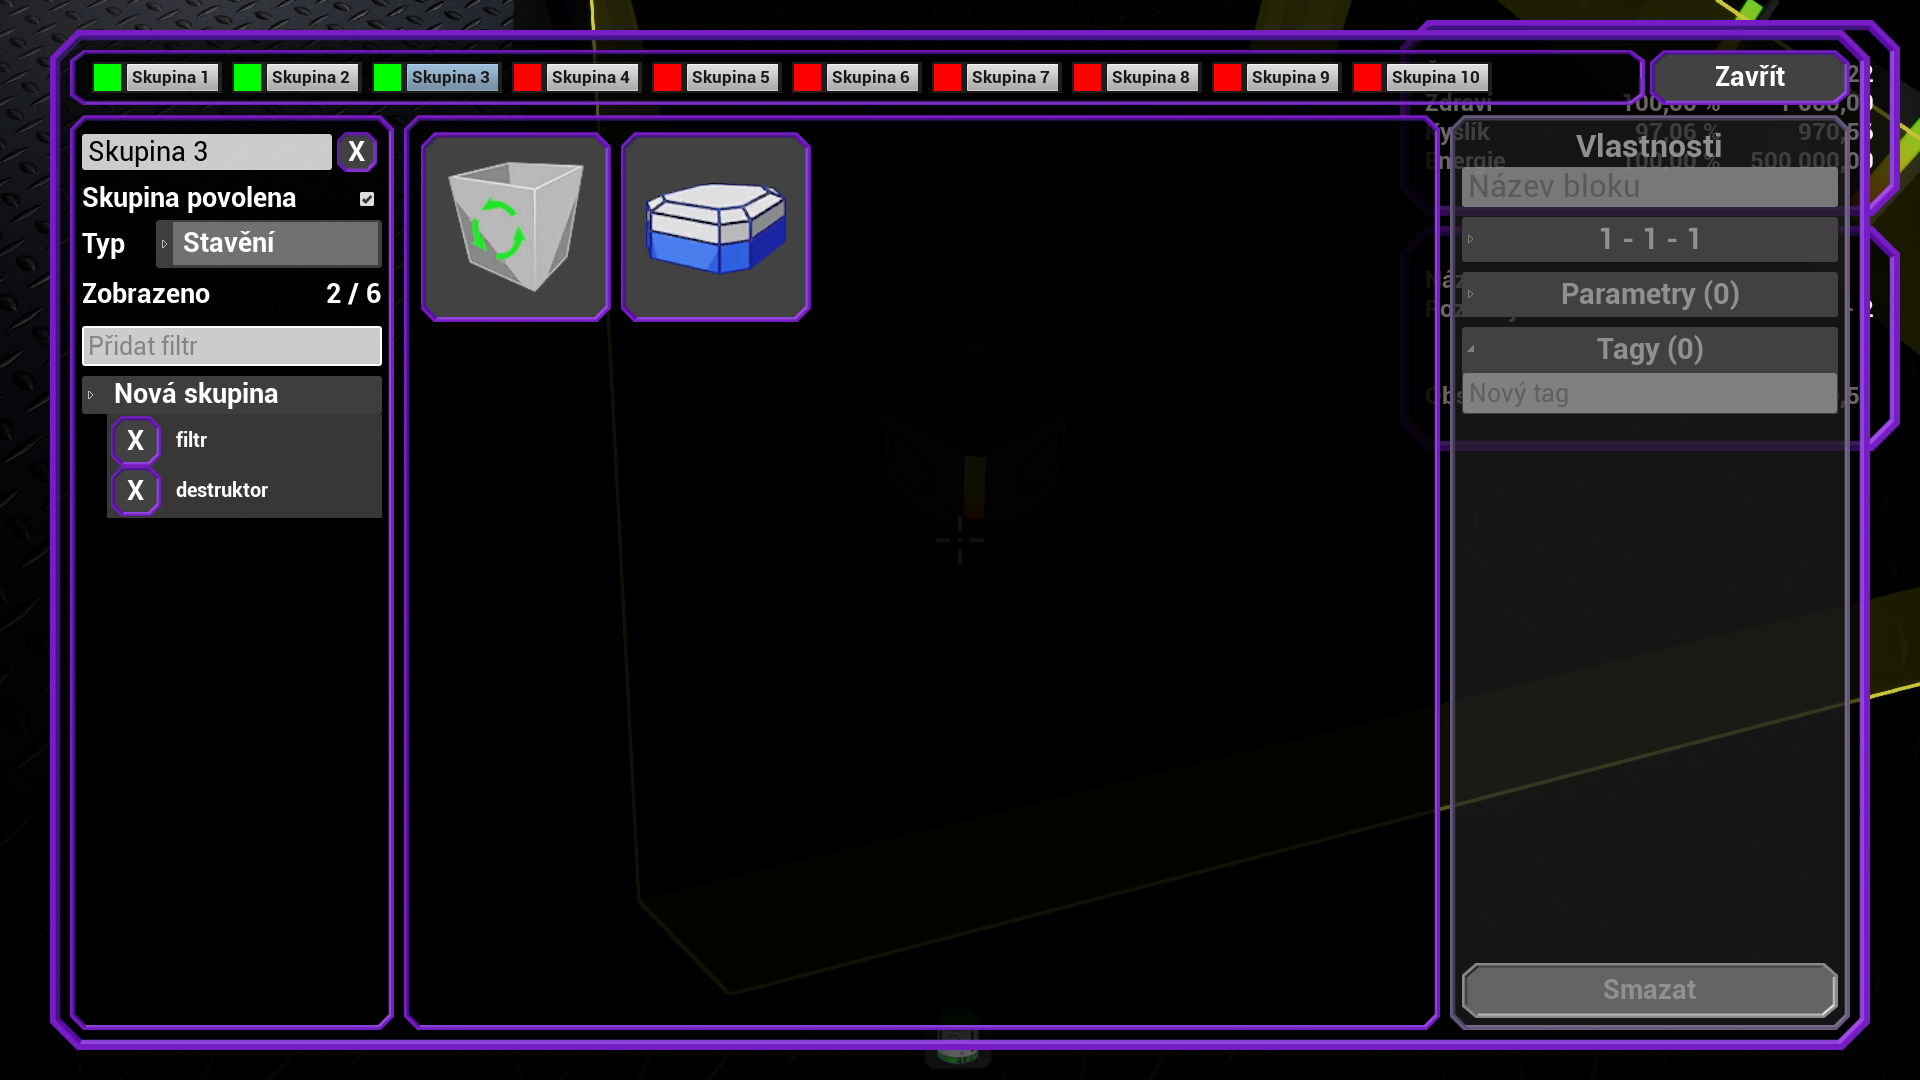
\includegraphics[ width=140mm]{../img/user/inventory/2filterResult}

\caption{Inventář - výsledek s filtrovanými položkami}
\label{fig:user_inventory_2filterResult}

\end{figure}

\FloatBarrier

Na následujícím obrázku je možné vidět filtry s rozbalenými vlastnostmi. Zaměřme se nyní na část \textit{Nesbalovat}. Po zaškrtnutí této volby je zobrazena pouze hlavička skupiny.

\begin{figure}[!ht]\centering
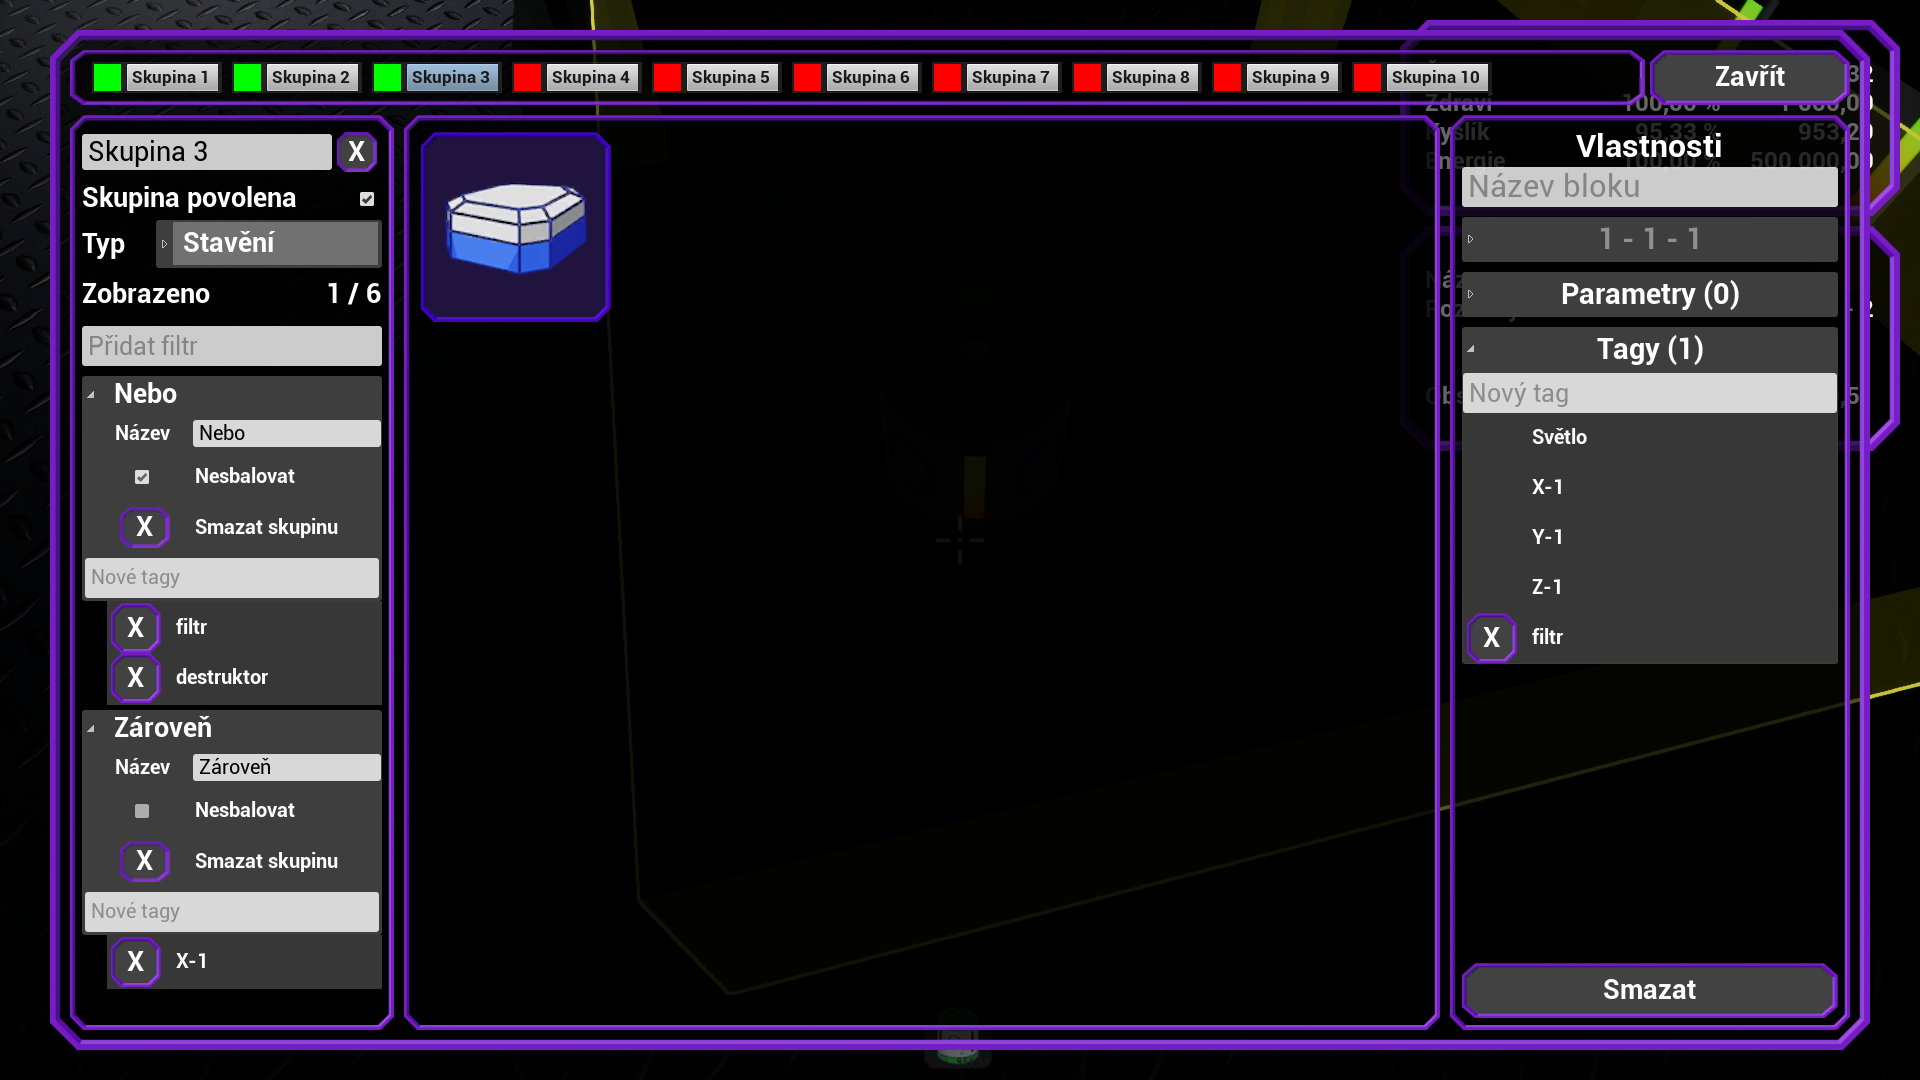
\includegraphics[ width=140mm]{../img/user/inventory/3additionalFilter}

\caption{Inventář - Nová hra}
\label{fig:user_inventory_3additionalFilter}

\end{figure}

\FloatBarrier

Výsledný seznam se sbalenými vlastnostmi filtru:

\begin{figure}[!ht]\centering
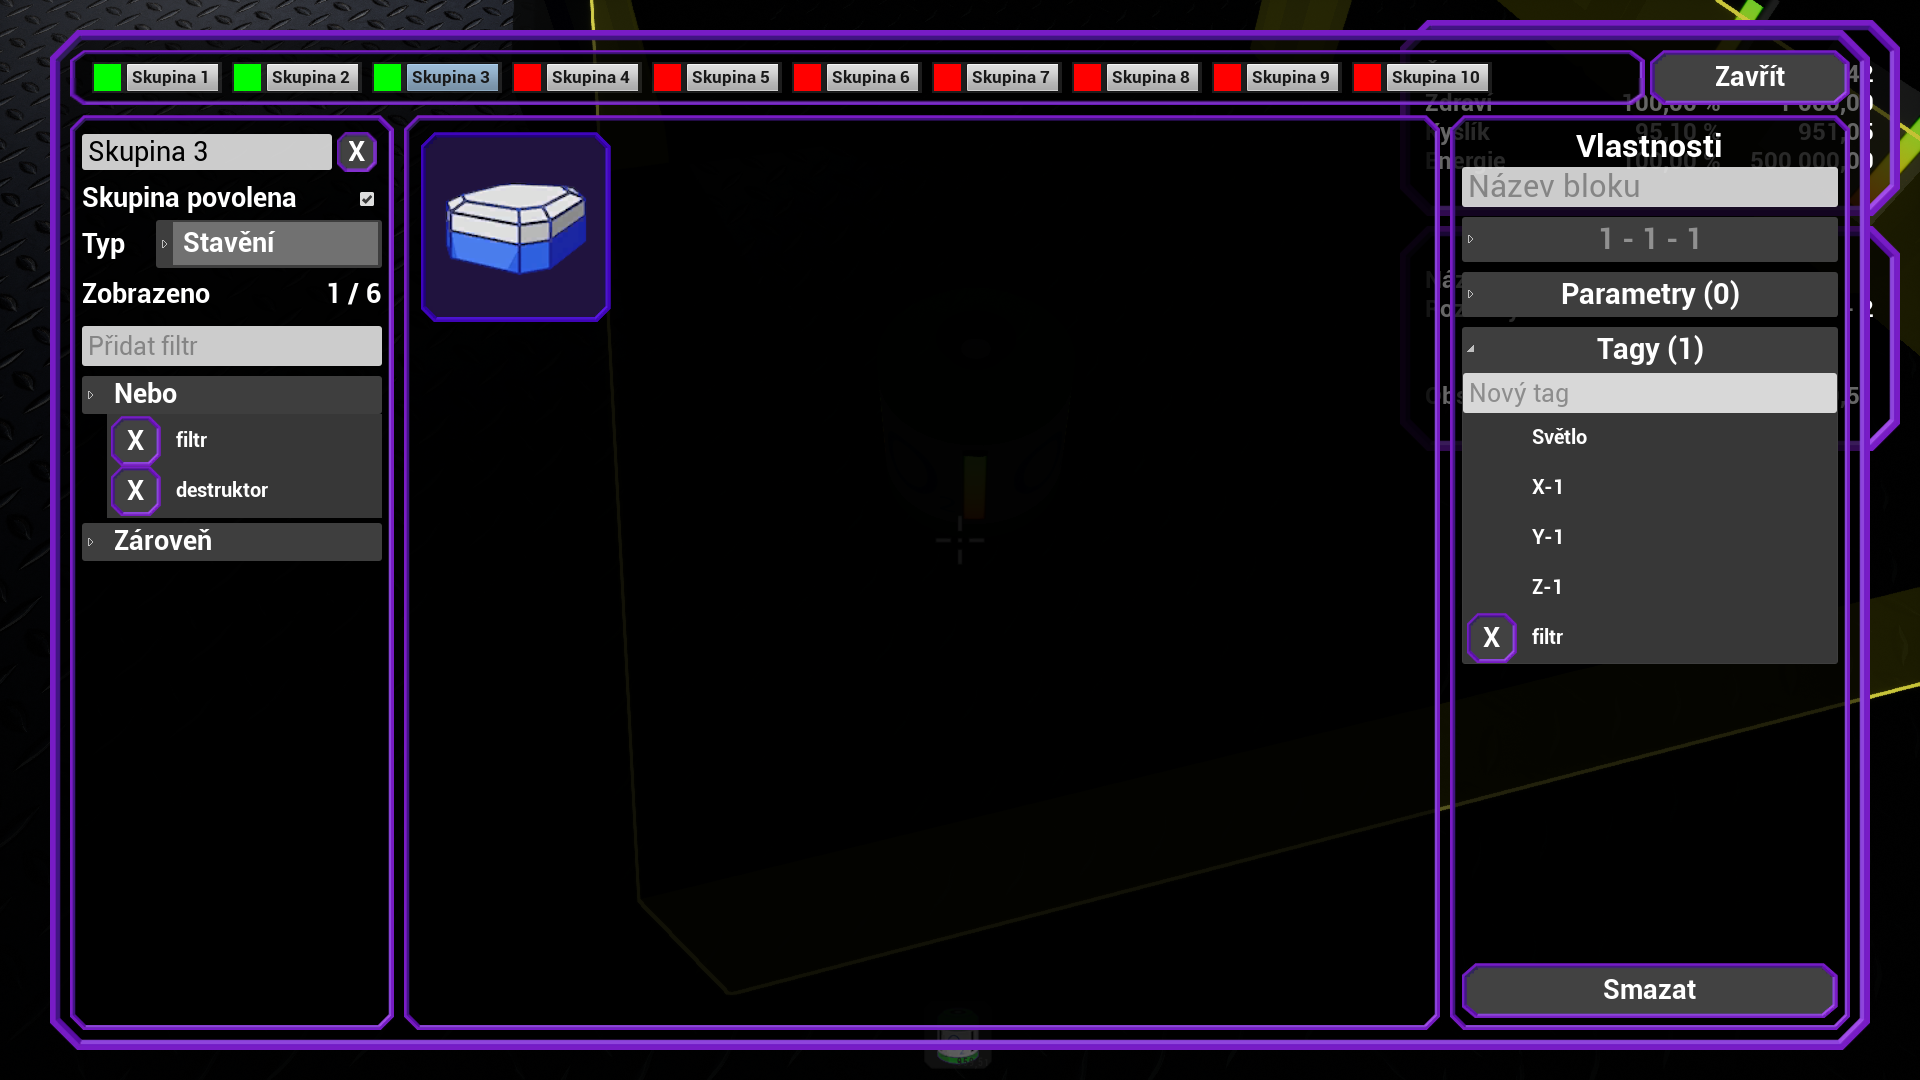
\includegraphics[ width=140mm]{../img/user/inventory/4addFilterCollapsed}

\caption{Inventář - Nahrát hru}
\label{fig:user_inventory_4addFilterCollapsed}

\end{figure}

\FloatBarrier

Označené položky je také možné smazat z inventáře. Umístitelné položky tak mohou být reálně zničeny. 

\begin{figure}[!ht]\centering
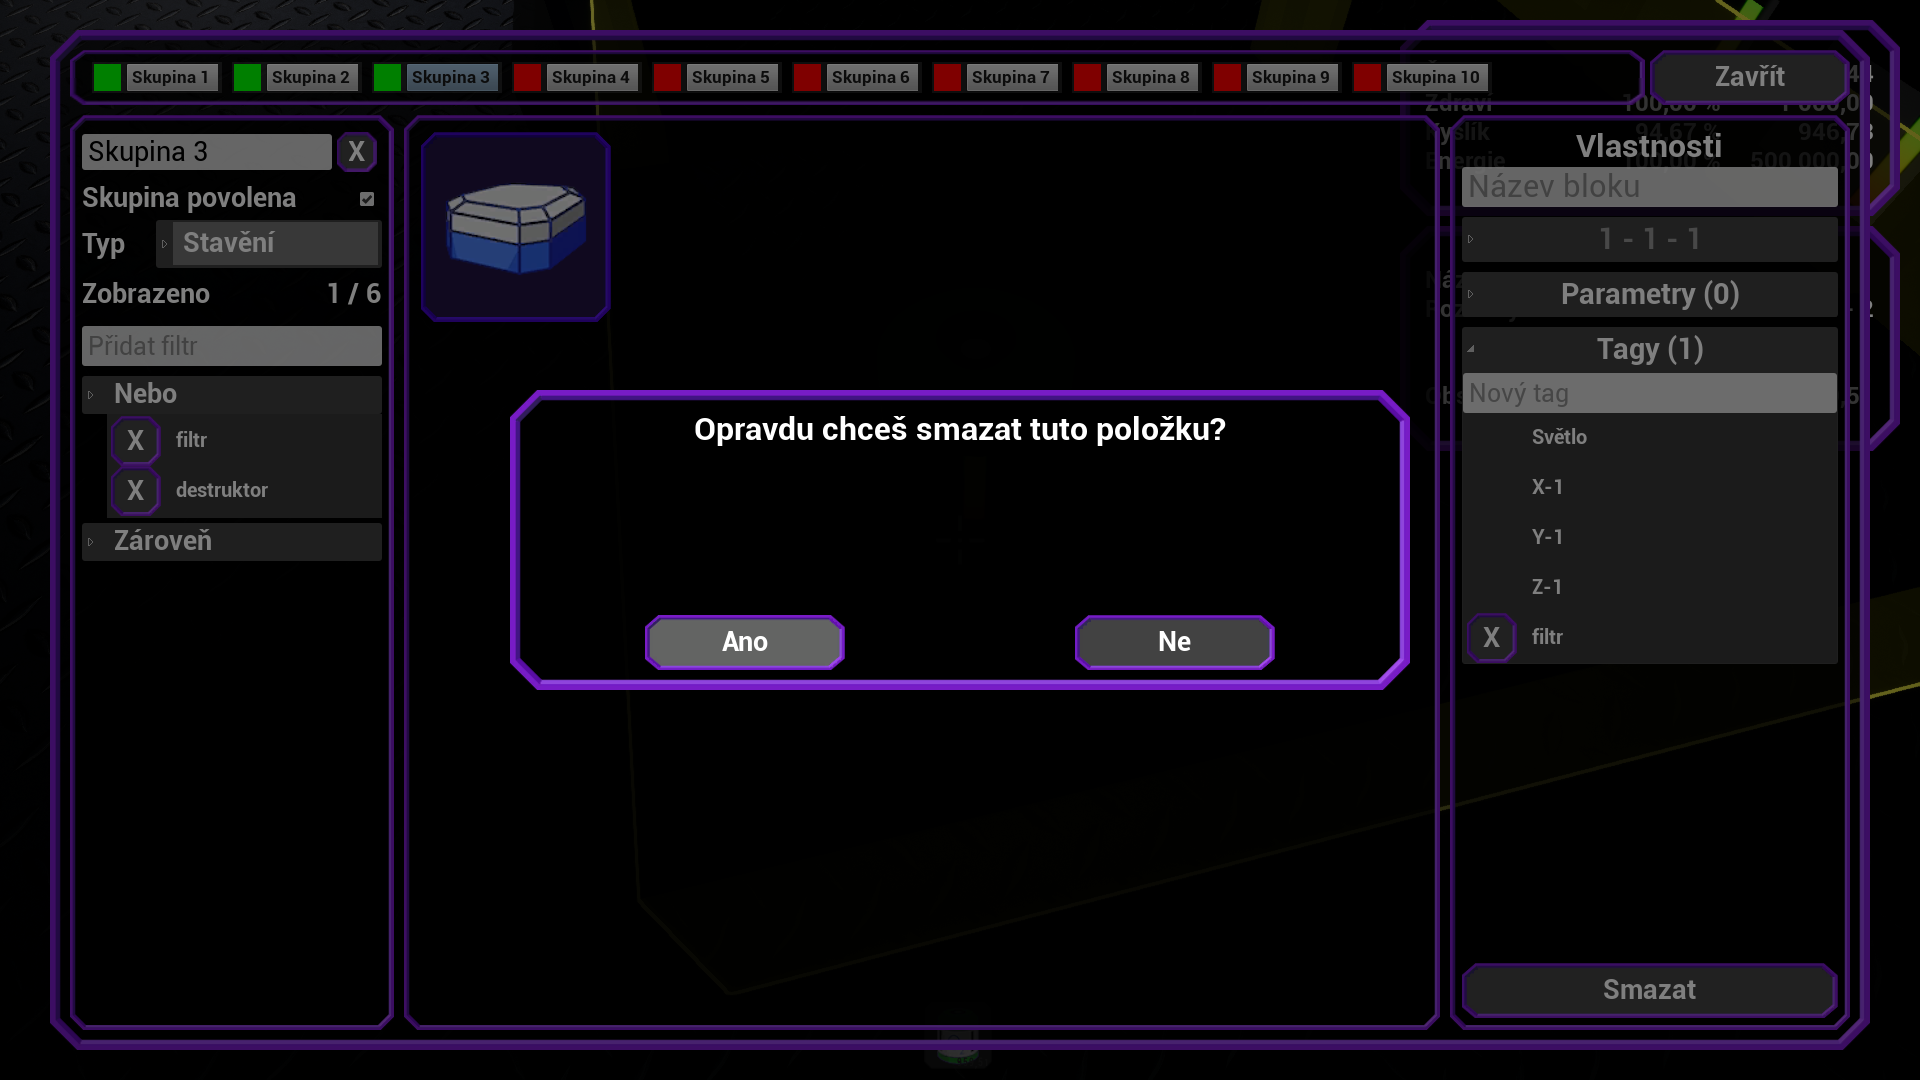
\includegraphics[ width=140mm]{../img/user/inventory/5deleteItem}

\caption{Inventář - Nastavení}
\label{fig:user_inventory_5deleteItem}

\end{figure}

\FloatBarrier
V případě, že je zvolena položka s dodatečnými parametry, je možné jejich hodnoty vidět v editoru vlastností bloku

\begin{figure}[!ht]\centering
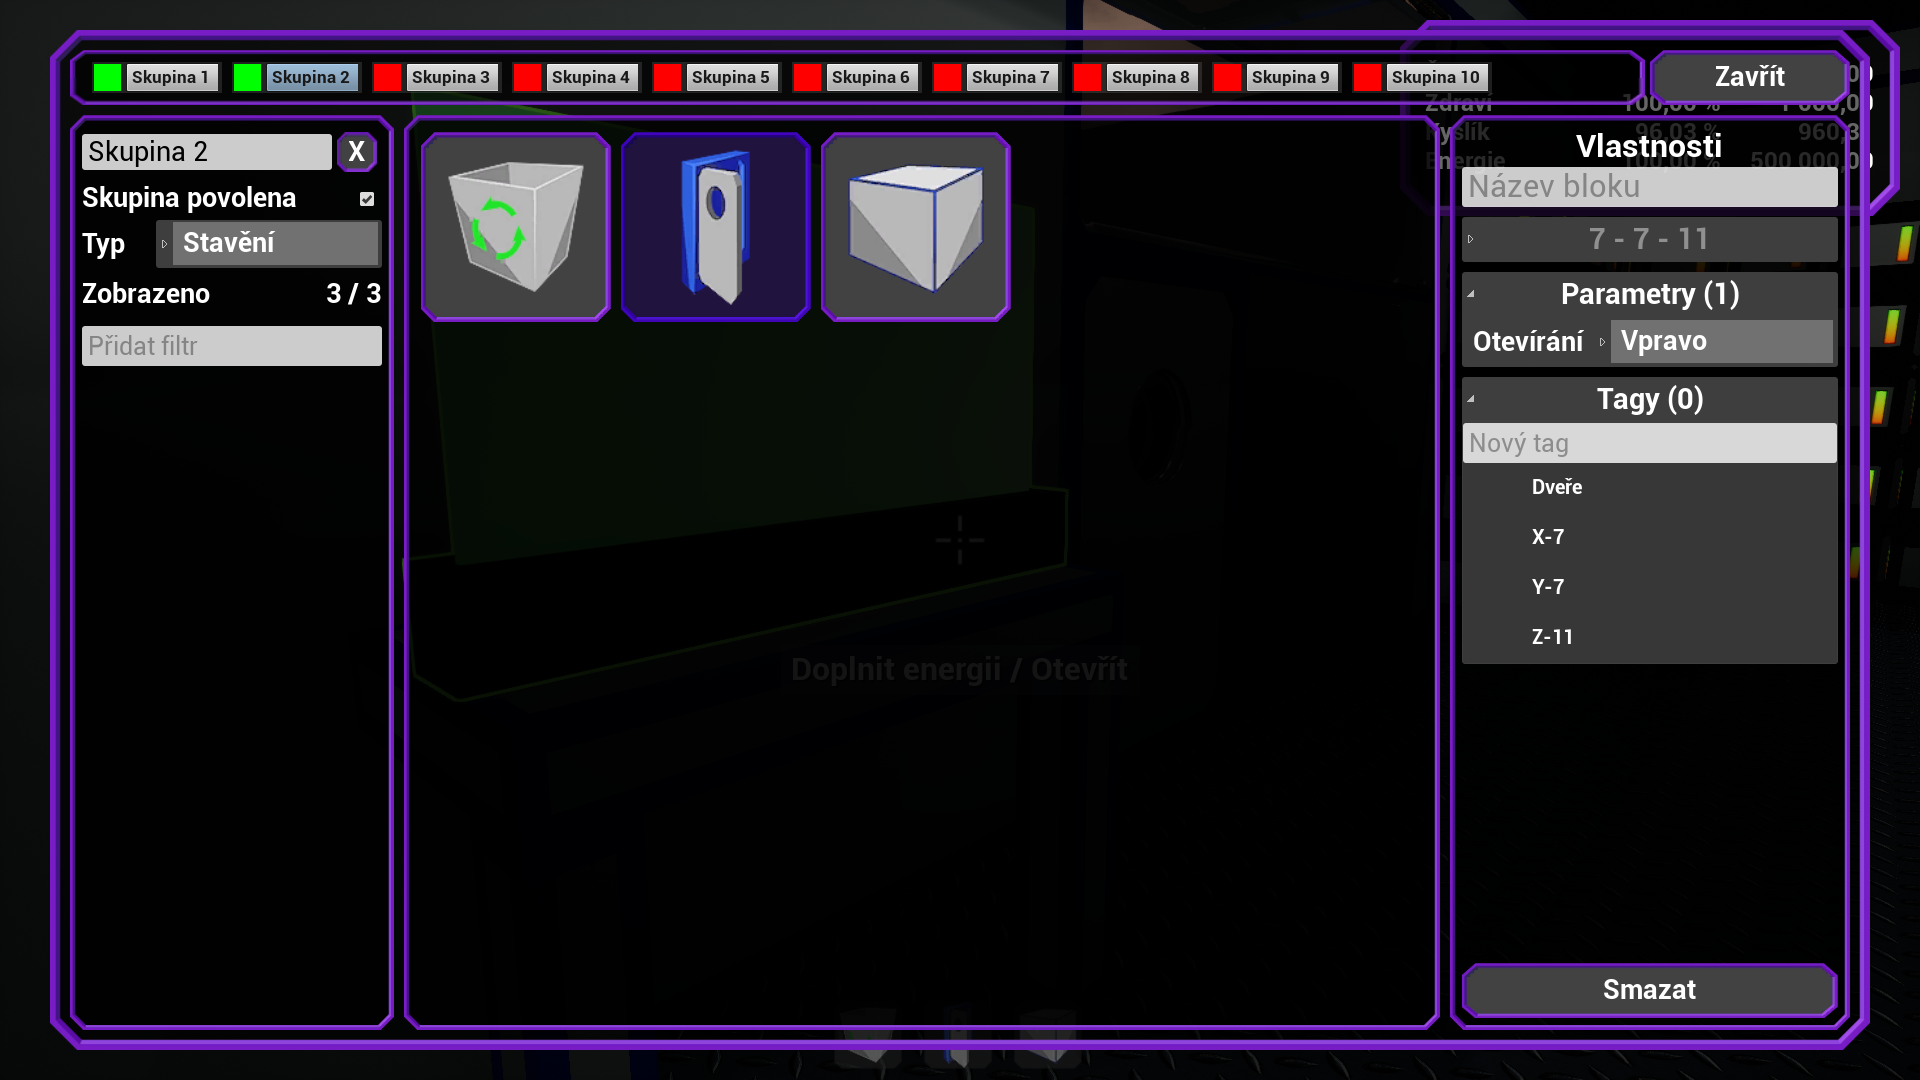
\includegraphics[ width=140mm]{../img/user/inventory/6itemWithParams}

\caption{Inventář - Nastavení}
\label{fig:user_inventory_6itemWithParams}

\end{figure}


\FloatBarrier
%!TEX root = ../prace.tex

\section{Terminál}

Pro informaci o aktuálním stavu sítě je nutné použít \textbf{Terminál}. Levým tlačítkem je možné rychle doplnit energii hráče, pravým pak otevřít ovládací obrazovku.

\begin{figure}[!h]\centering
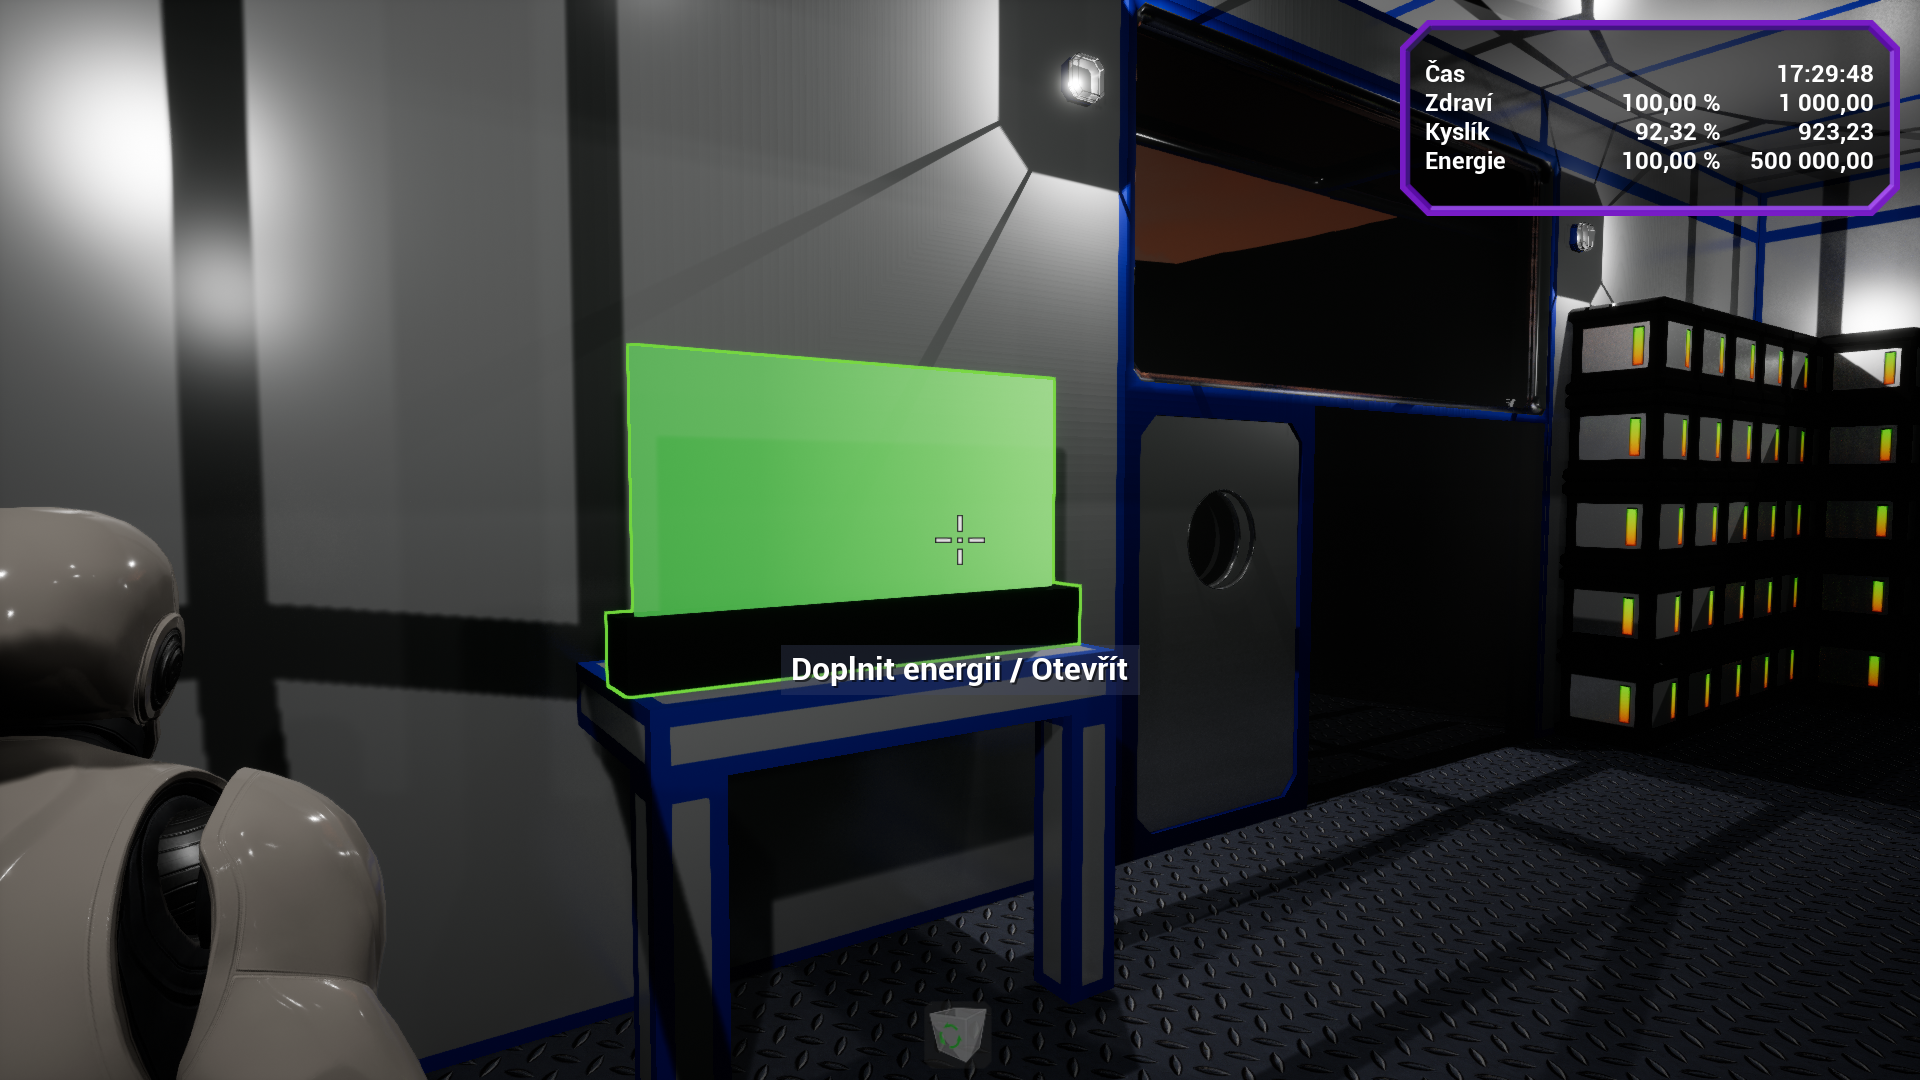
\includegraphics[ width=140mm]{../img/user/terminal/0terminalOverall}

\caption{Terminál - ve hře}
\label{fig:user_terminal_0terminalOverall}

\end{figure}

\FloatBarrier

V \textit{horní} části je vidět selektor obrazovky. Jeho rozkliknutím (více v obrázku \ref{fig:user_terminal_3terminalCtorSelector}) je možné zvolit výchozí obrazovku, nebo jeden z \textbf{Konstruktoru objektů}, které jsou v dispozici v síti.




\begin{figure}[!h]\centering
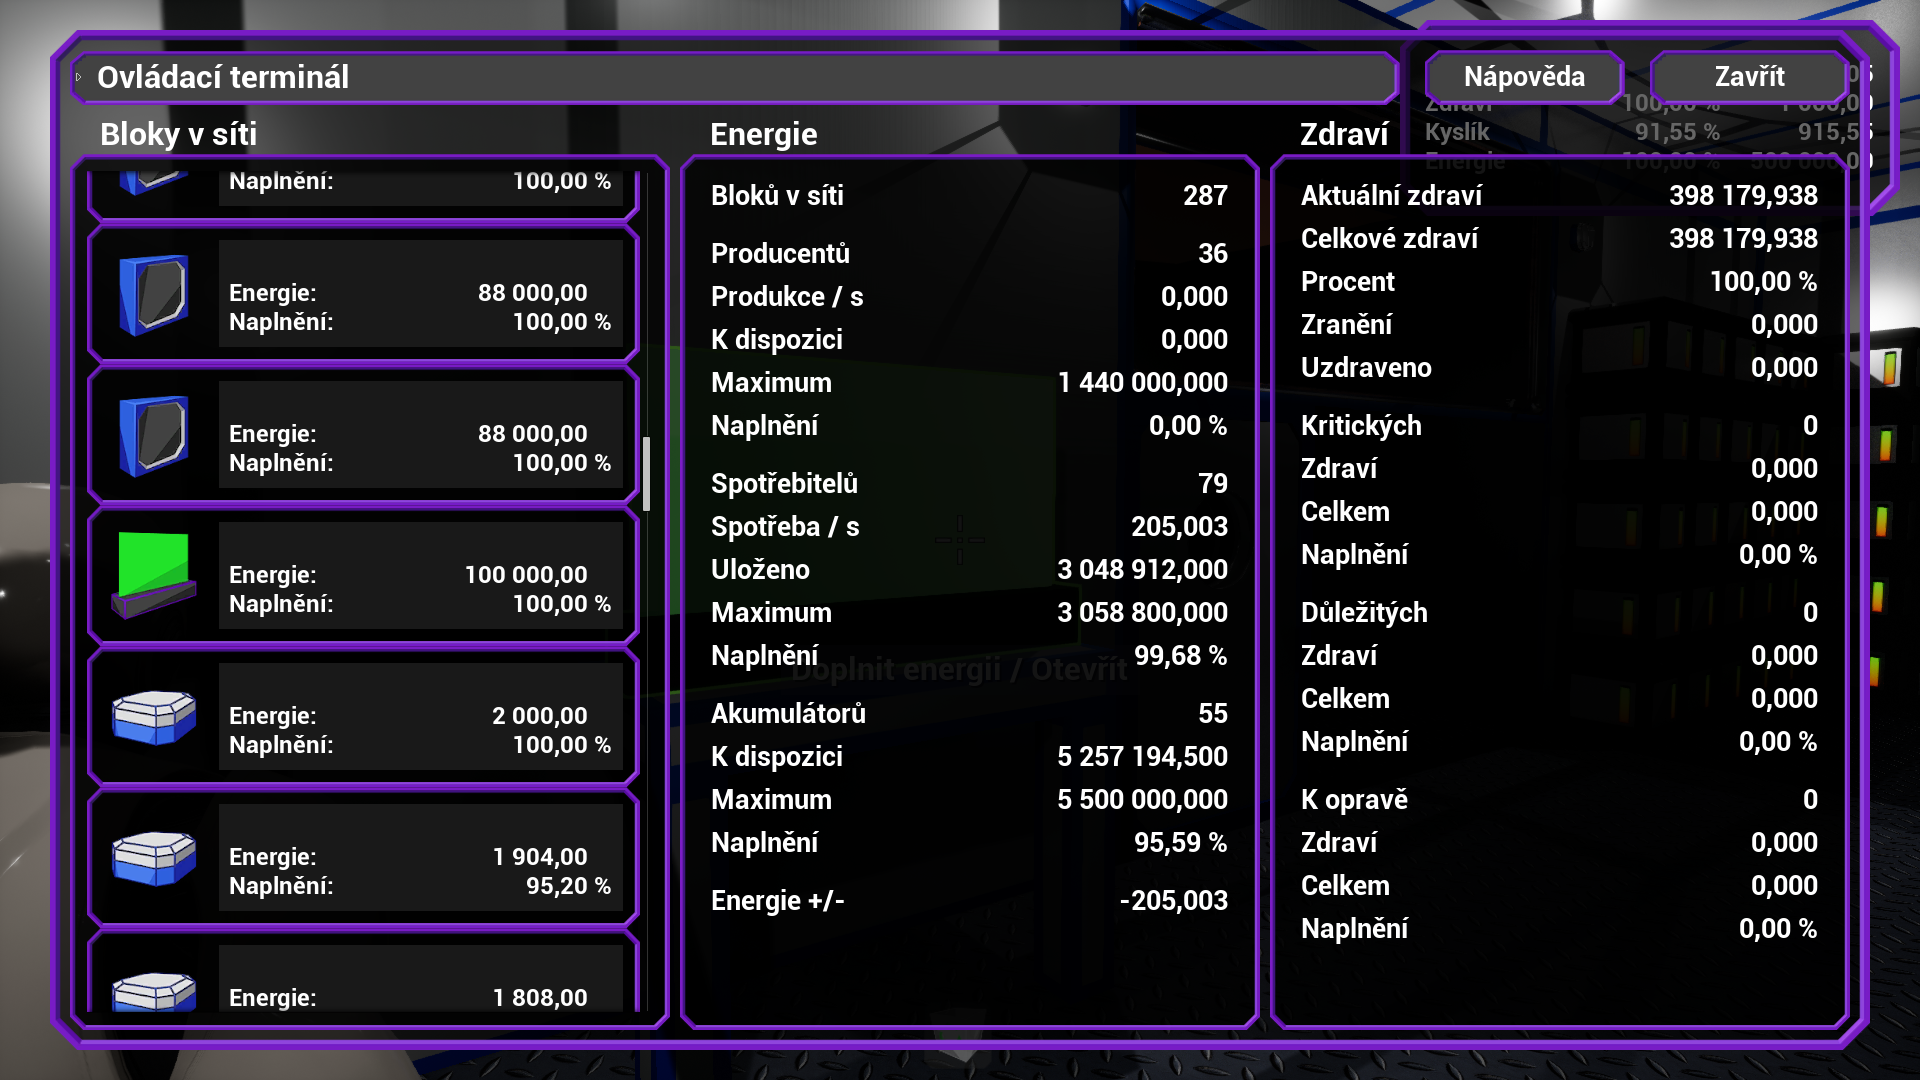
\includegraphics[ width=140mm]{../img/user/terminal/1terminalInfo}

\caption{Terminál - výchozí obrazovka}
\label{fig:user_terminal_1terminalInfo}

\end{figure}

\FloatBarrier
V \textit{levé} části je vidět seznam význačných bloků. \textit{Uprostřed} jsou vidět energetické informace o síti. \textit{Vpravo} je pak možné sledovat aktuální zdravotní stav sítě a bloků v síti.

Tlačítkem \textbf{Nápověda} je možné zobrazit informace o ovládání hry a přiřazených klávesách pro jednotlivé úkony.

\begin{figure}[!h]\centering
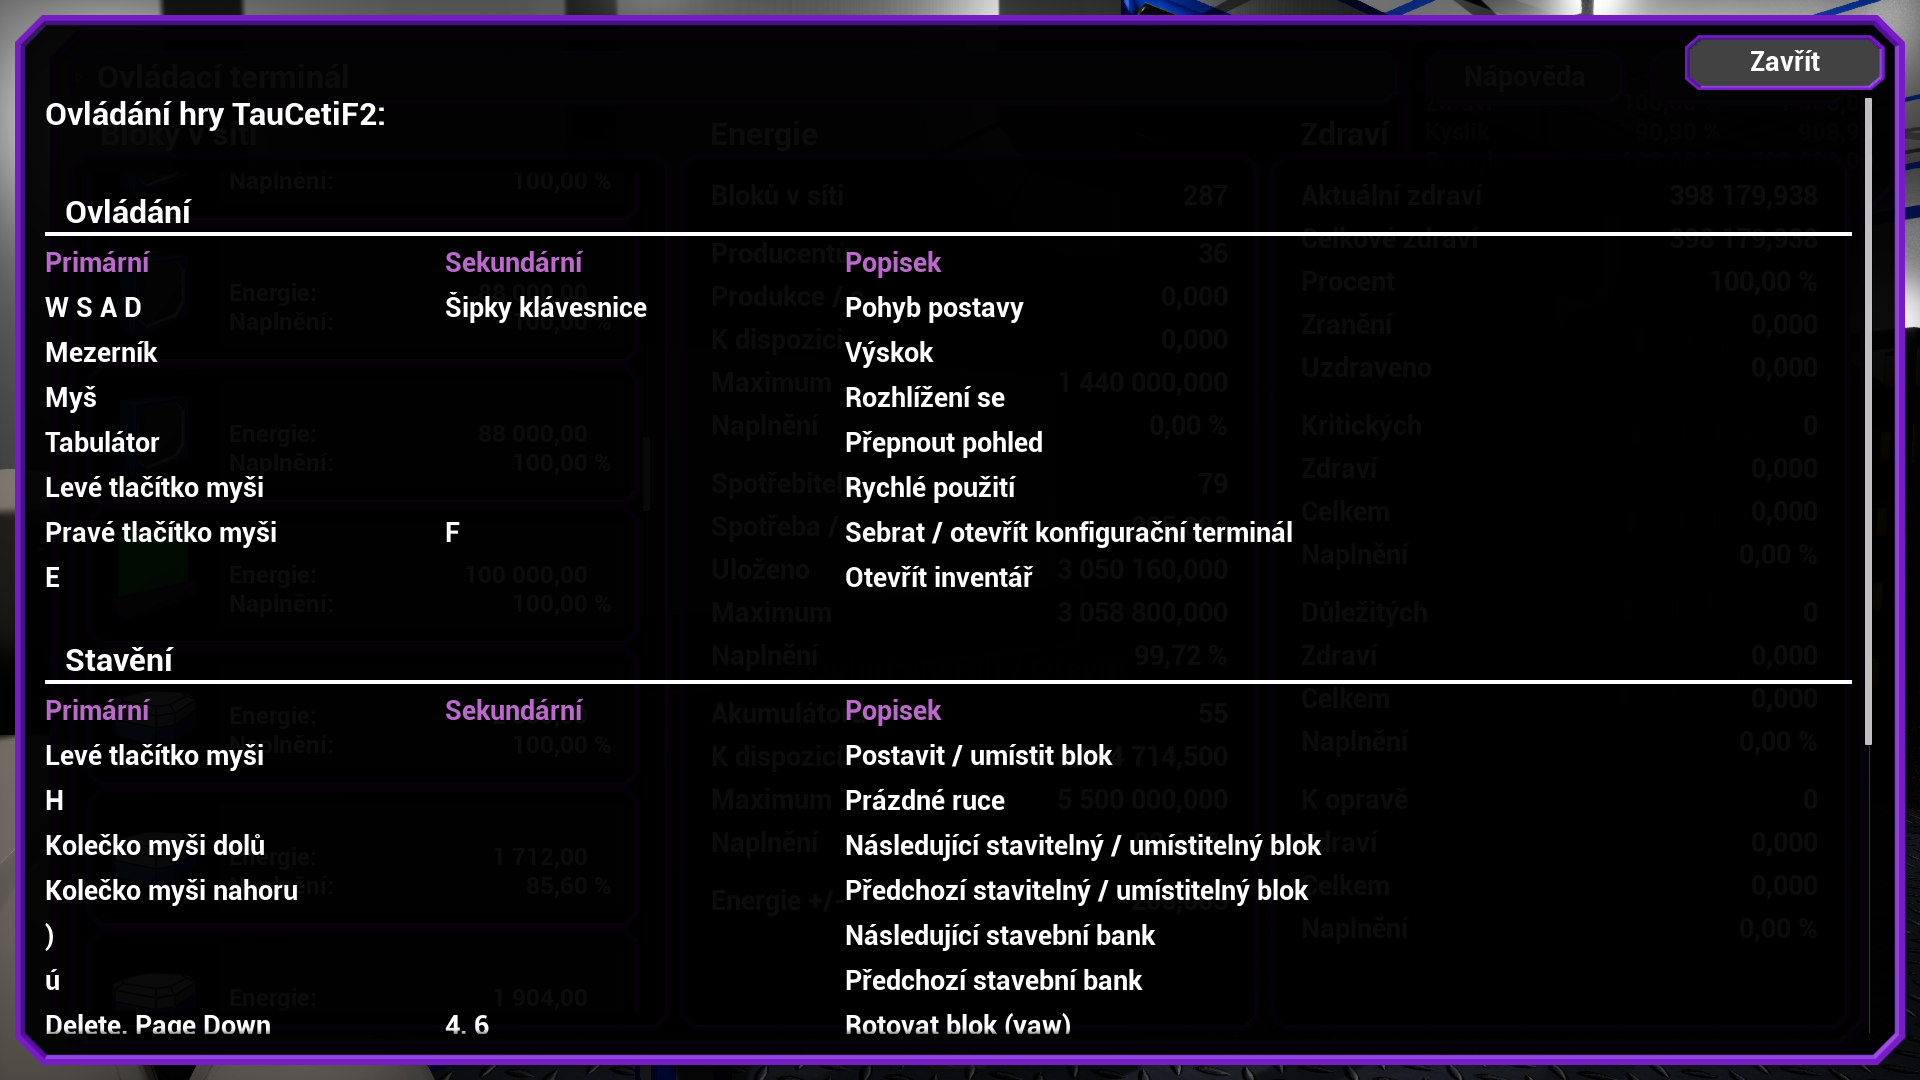
\includegraphics[ width=140mm]{../img/user/terminal/2terminalHelp}

\caption{Terminál - nápověda}
\label{fig:user_terminal_2terminalHelp}

\end{figure}

\FloatBarrier

Selektor dostupných obrazovek:

\begin{figure}[!h]\centering
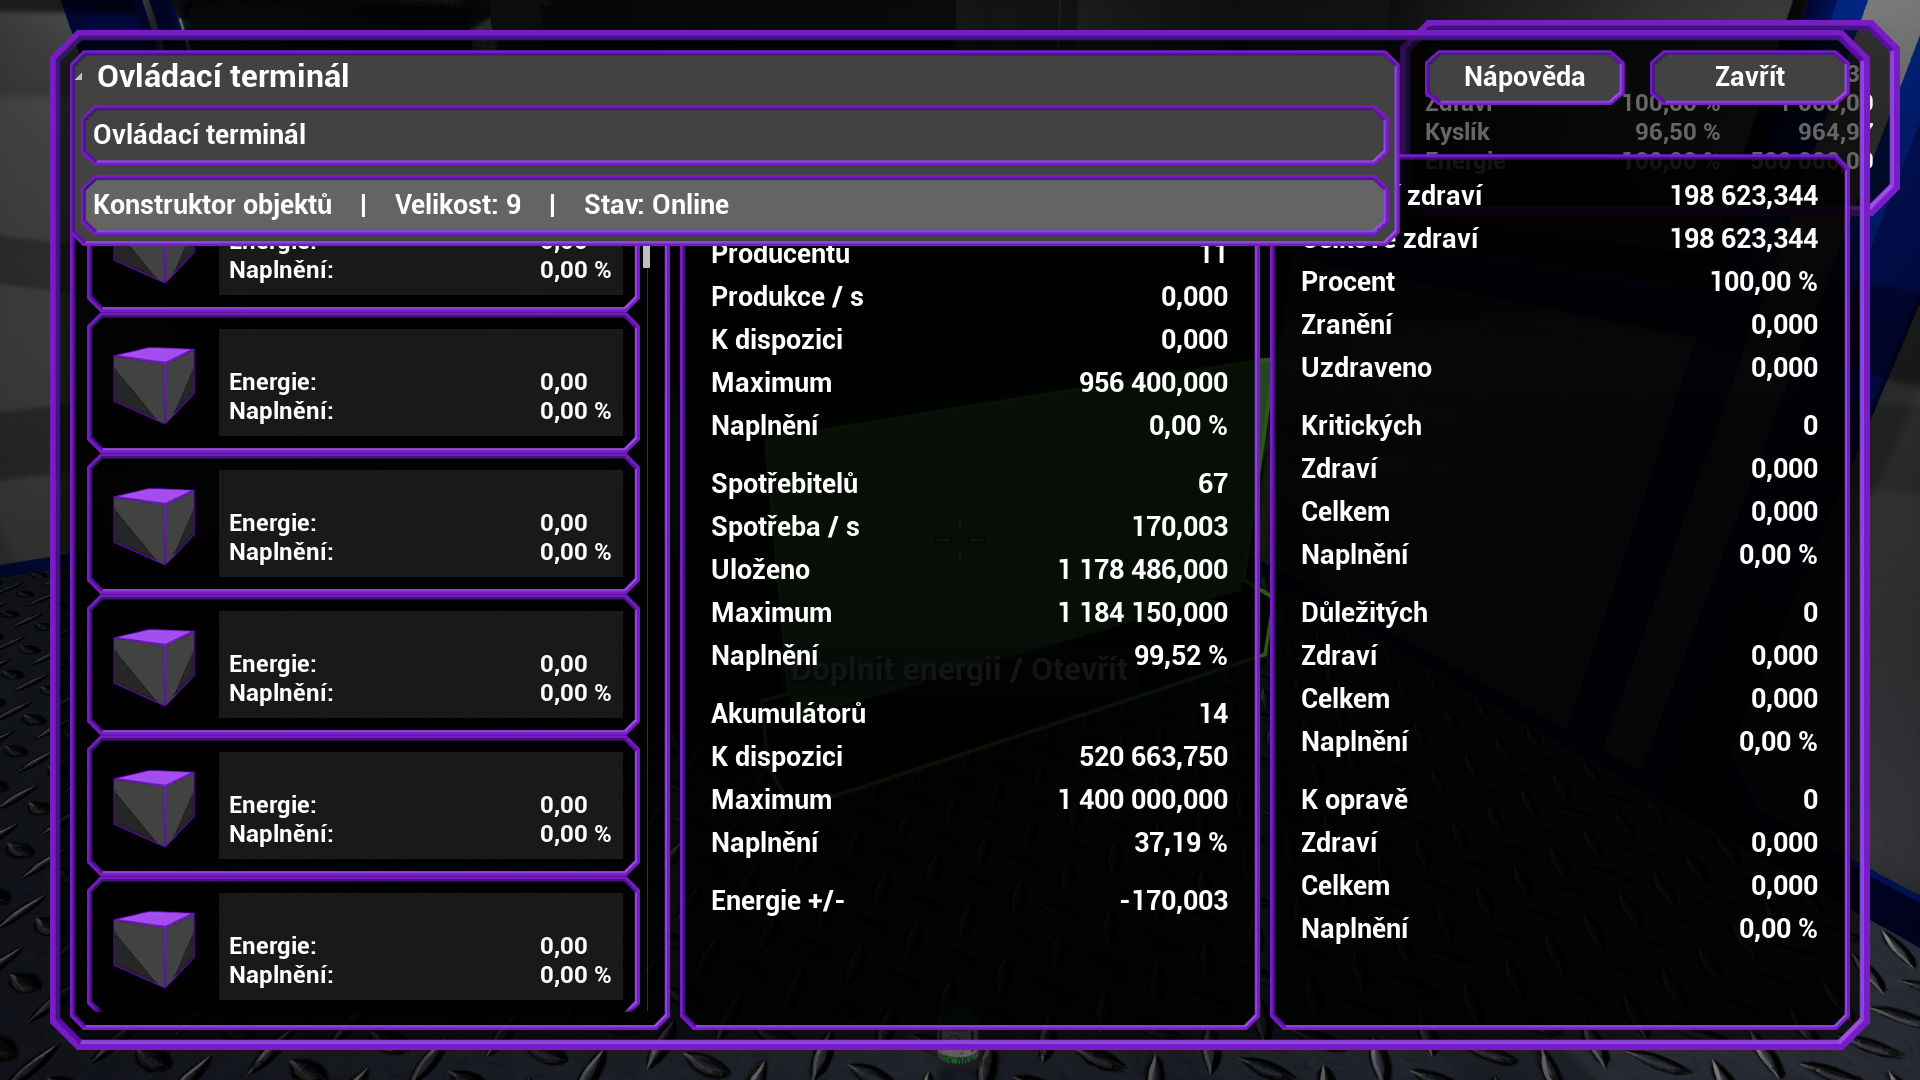
\includegraphics[ width=140mm]{../img/user/terminal/3terminalCtorSelector}

\caption{Terminál - selektor obrazovek}
\label{fig:user_terminal_3terminalCtorSelector}

\end{figure}

\FloatBarrier

Pokud vybereme \textbf{Konstruktor objektů}, vidíme seznam dostupných bloků, které můžeme zkonstruovat. Pokud to pro některé nelze (třeba z důvodu omezení velikosti - konstruktor je na daný objekt příliš malý), blok není aktivní a nelze ho zvolit.


\begin{figure}[!h]\centering
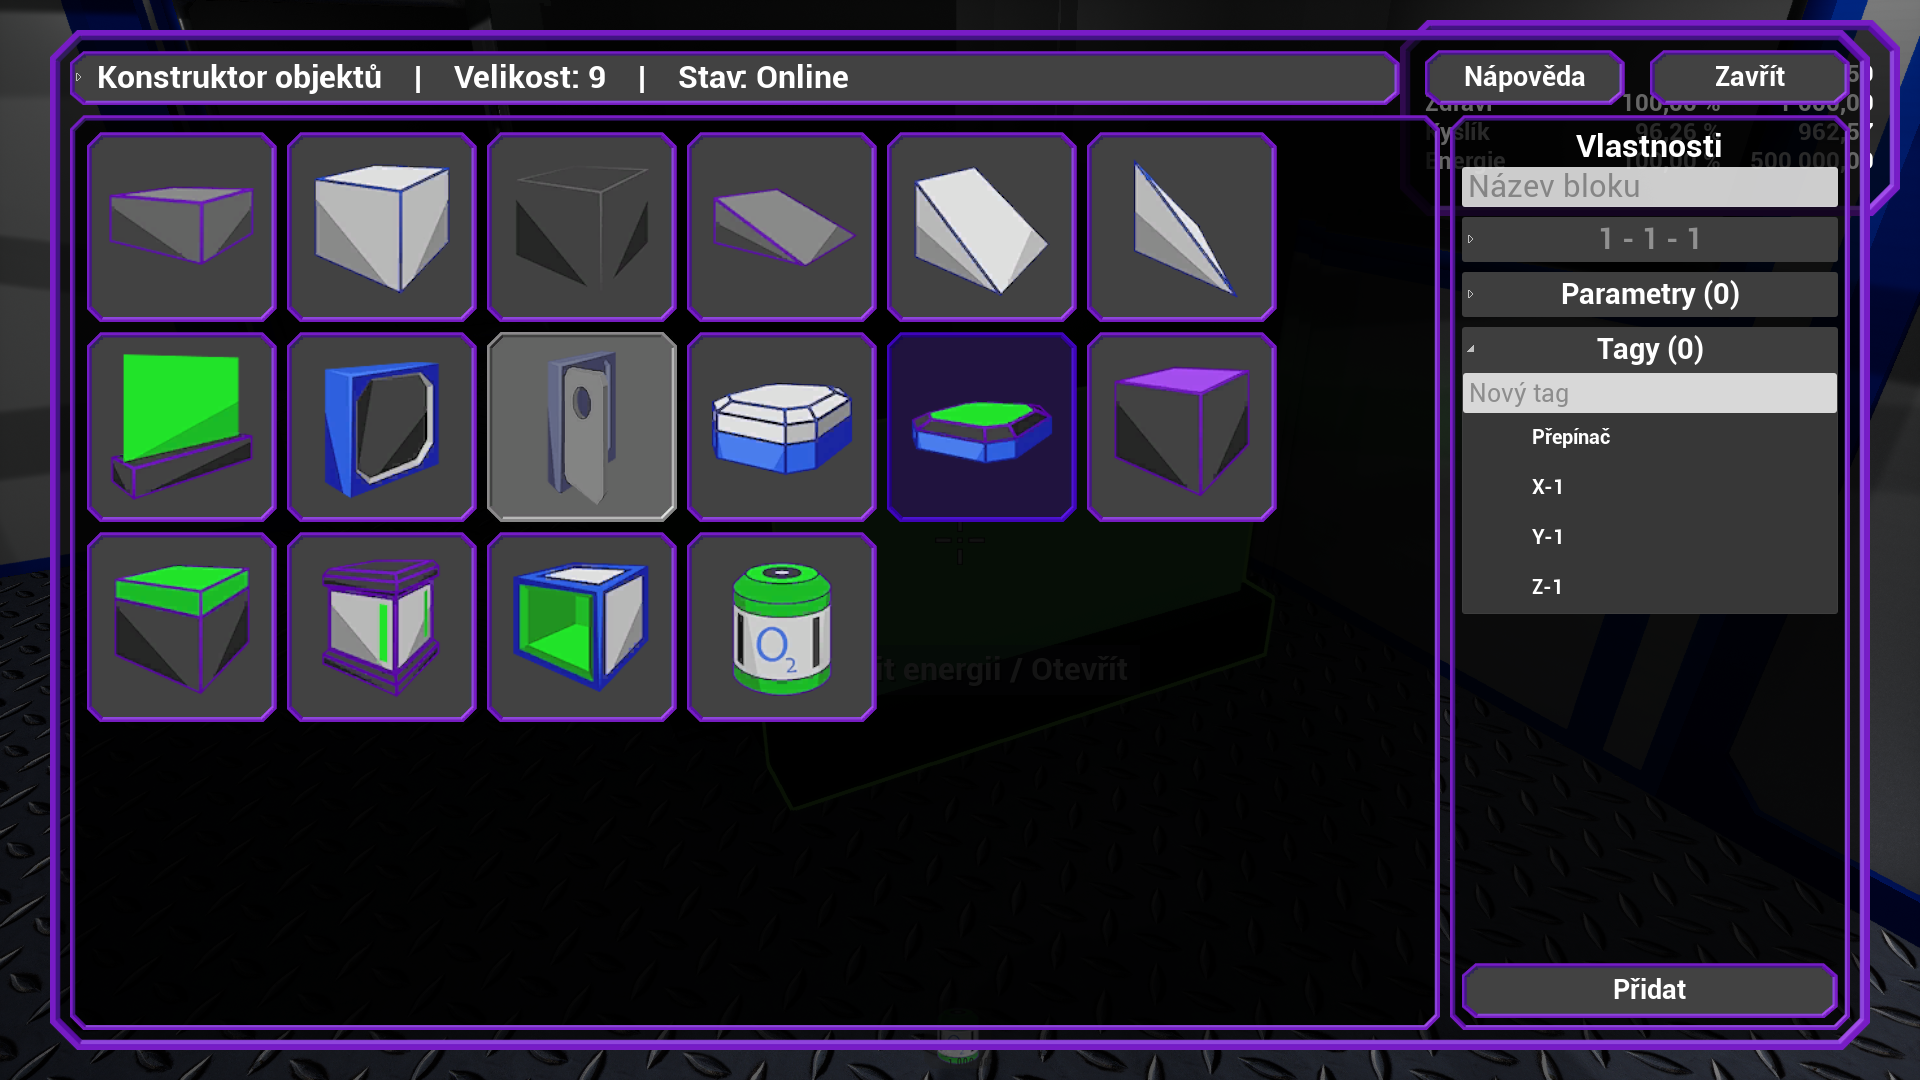
\includegraphics[ width=140mm]{../img/user/terminal/4builderSmall}

\caption{Terminál - konstruktor objektů}
\label{fig:user_terminal_4builderSmall}

\end{figure}

\FloatBarrier

V sekci \textit{Nastavení} je možné kromě tagů definovat i požadovanou velikost a to až do velikosti konstruktoru, nebo globálního omezení 20 násobku  základní kostky.

\begin{figure}[!h]\centering
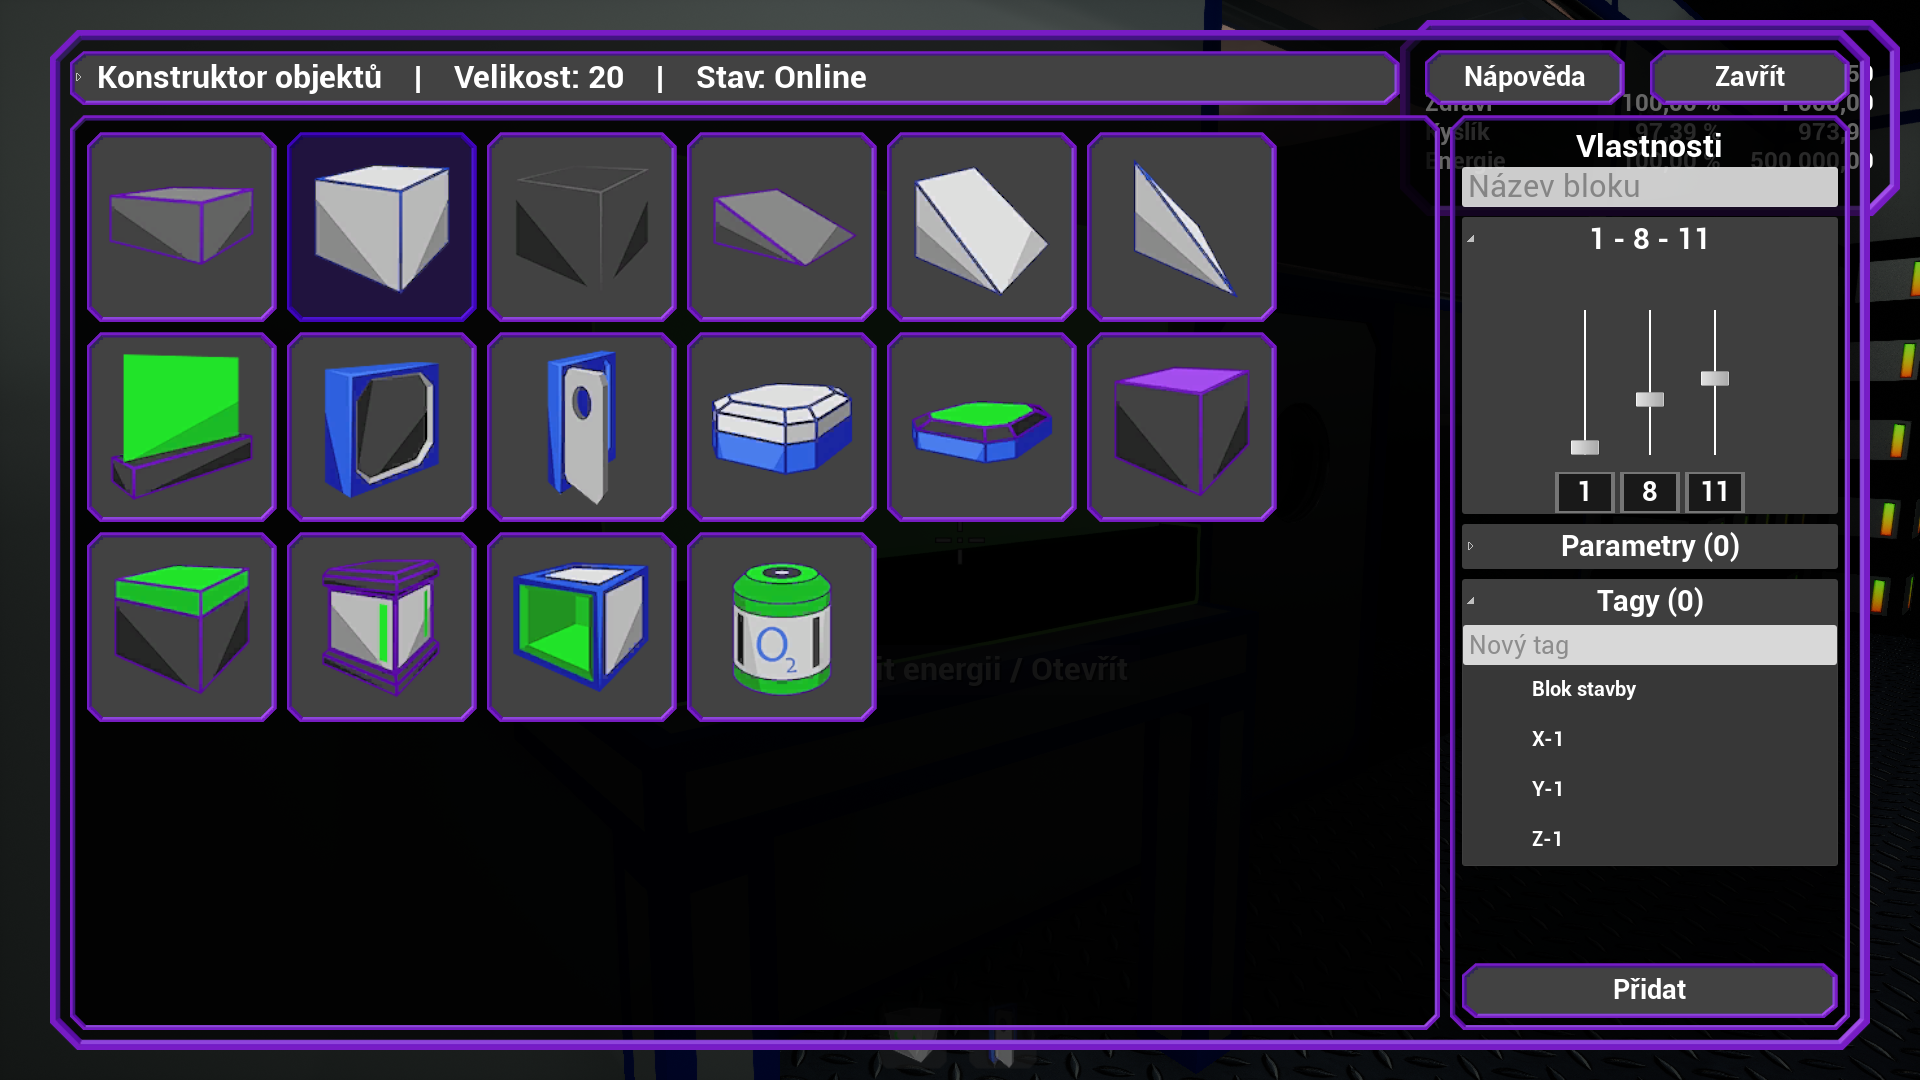
\includegraphics[ width=140mm]{../img/user/terminal/5builderSize}

\caption{Terminál - Nastavení velikosti}
\label{fig:user_terminal_5builderSize}

\end{figure}

\FloatBarrier

Některé bloky, třeba \textbf{Dveře} požadují dodatečné parametry, které ovlivňují jejich výsledné chování. V našem případě to je smysl otevírání dveří při čelním pohledu. Na obrázku je vidět stav po rozkliknutí.

\begin{figure}[!h]\centering
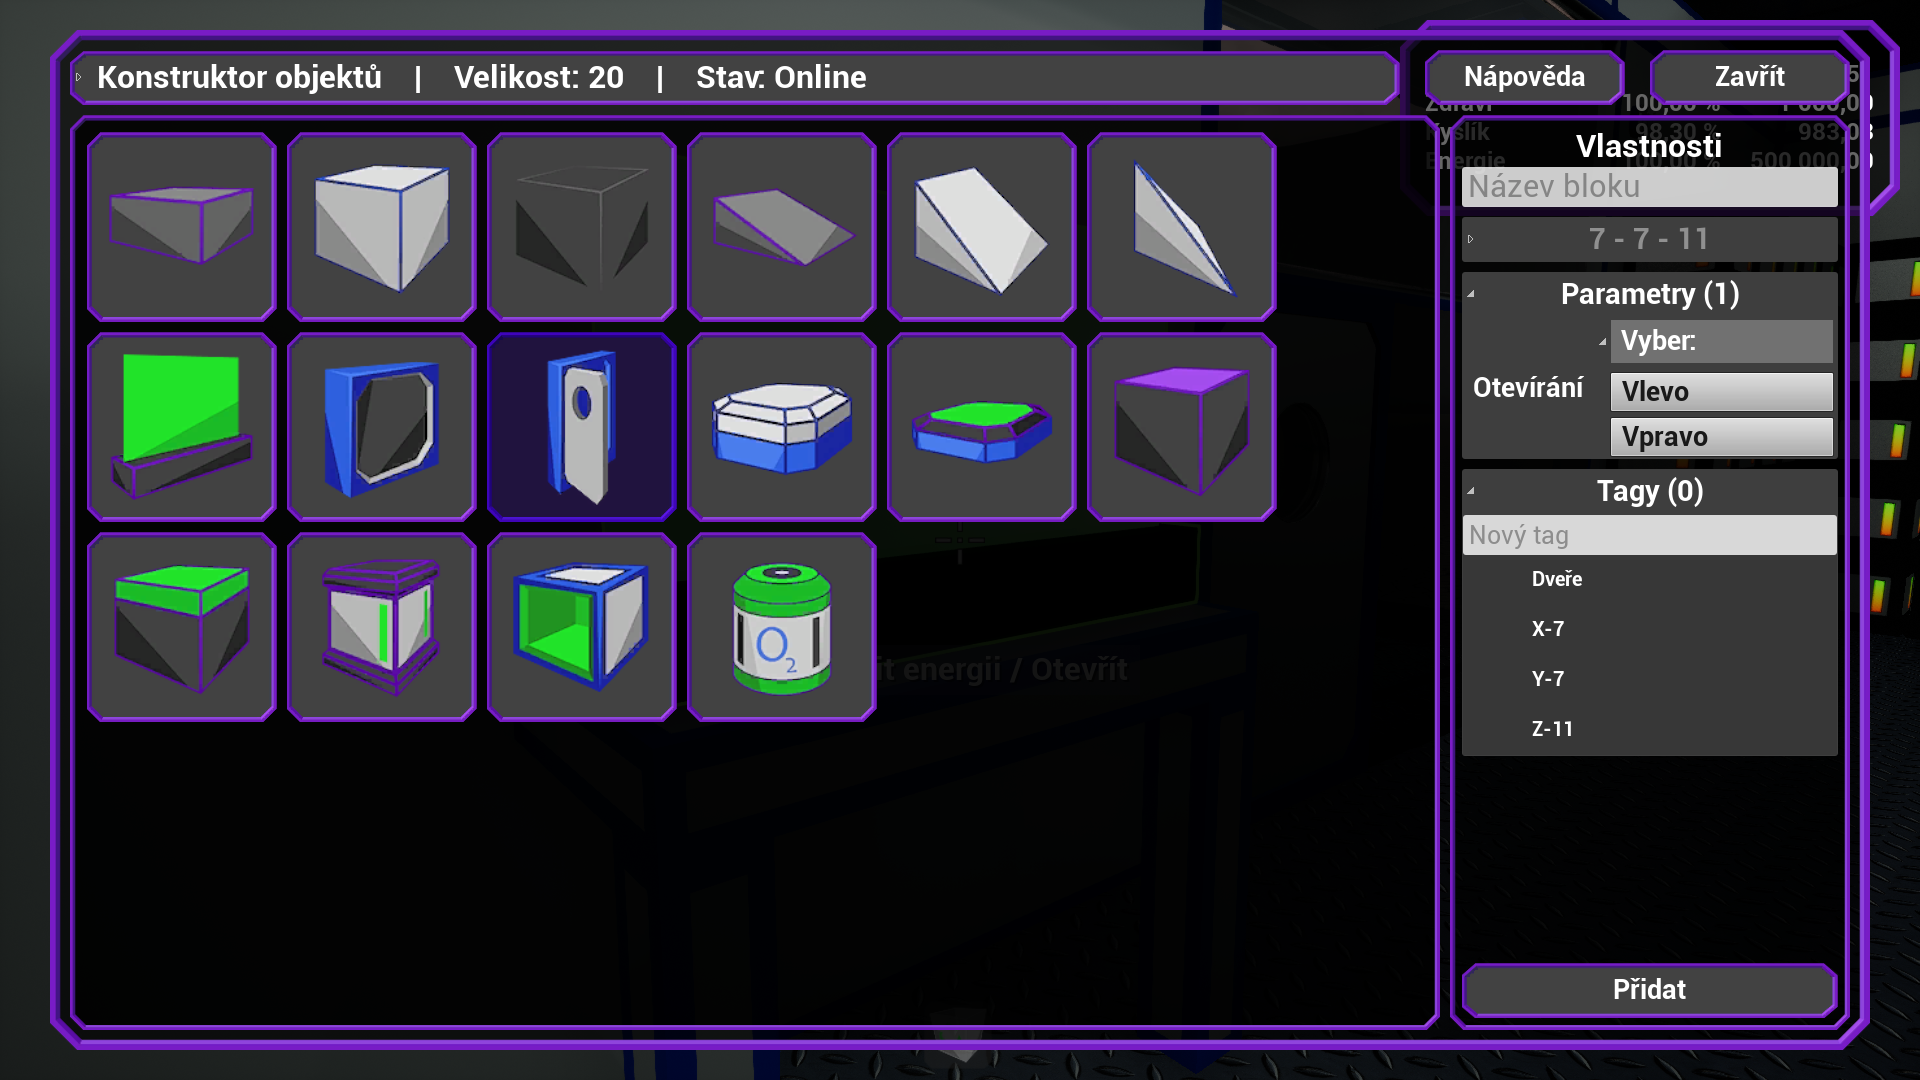
\includegraphics[ width=140mm]{../img/user/terminal/6builderParams}

\caption{Terminál - Nastavení parametrů}
\label{fig:user_terminal_6builderParams}

\end{figure}

\FloatBarrier
%!TEX root = ../../prace.tex

\section{Stavební akce}

\textbf{Destruktor} umožňuje mazat bloky. Po jeho výběru je vidět červený outline vybraného bloku.

\begin{figure}[!ht]\centering
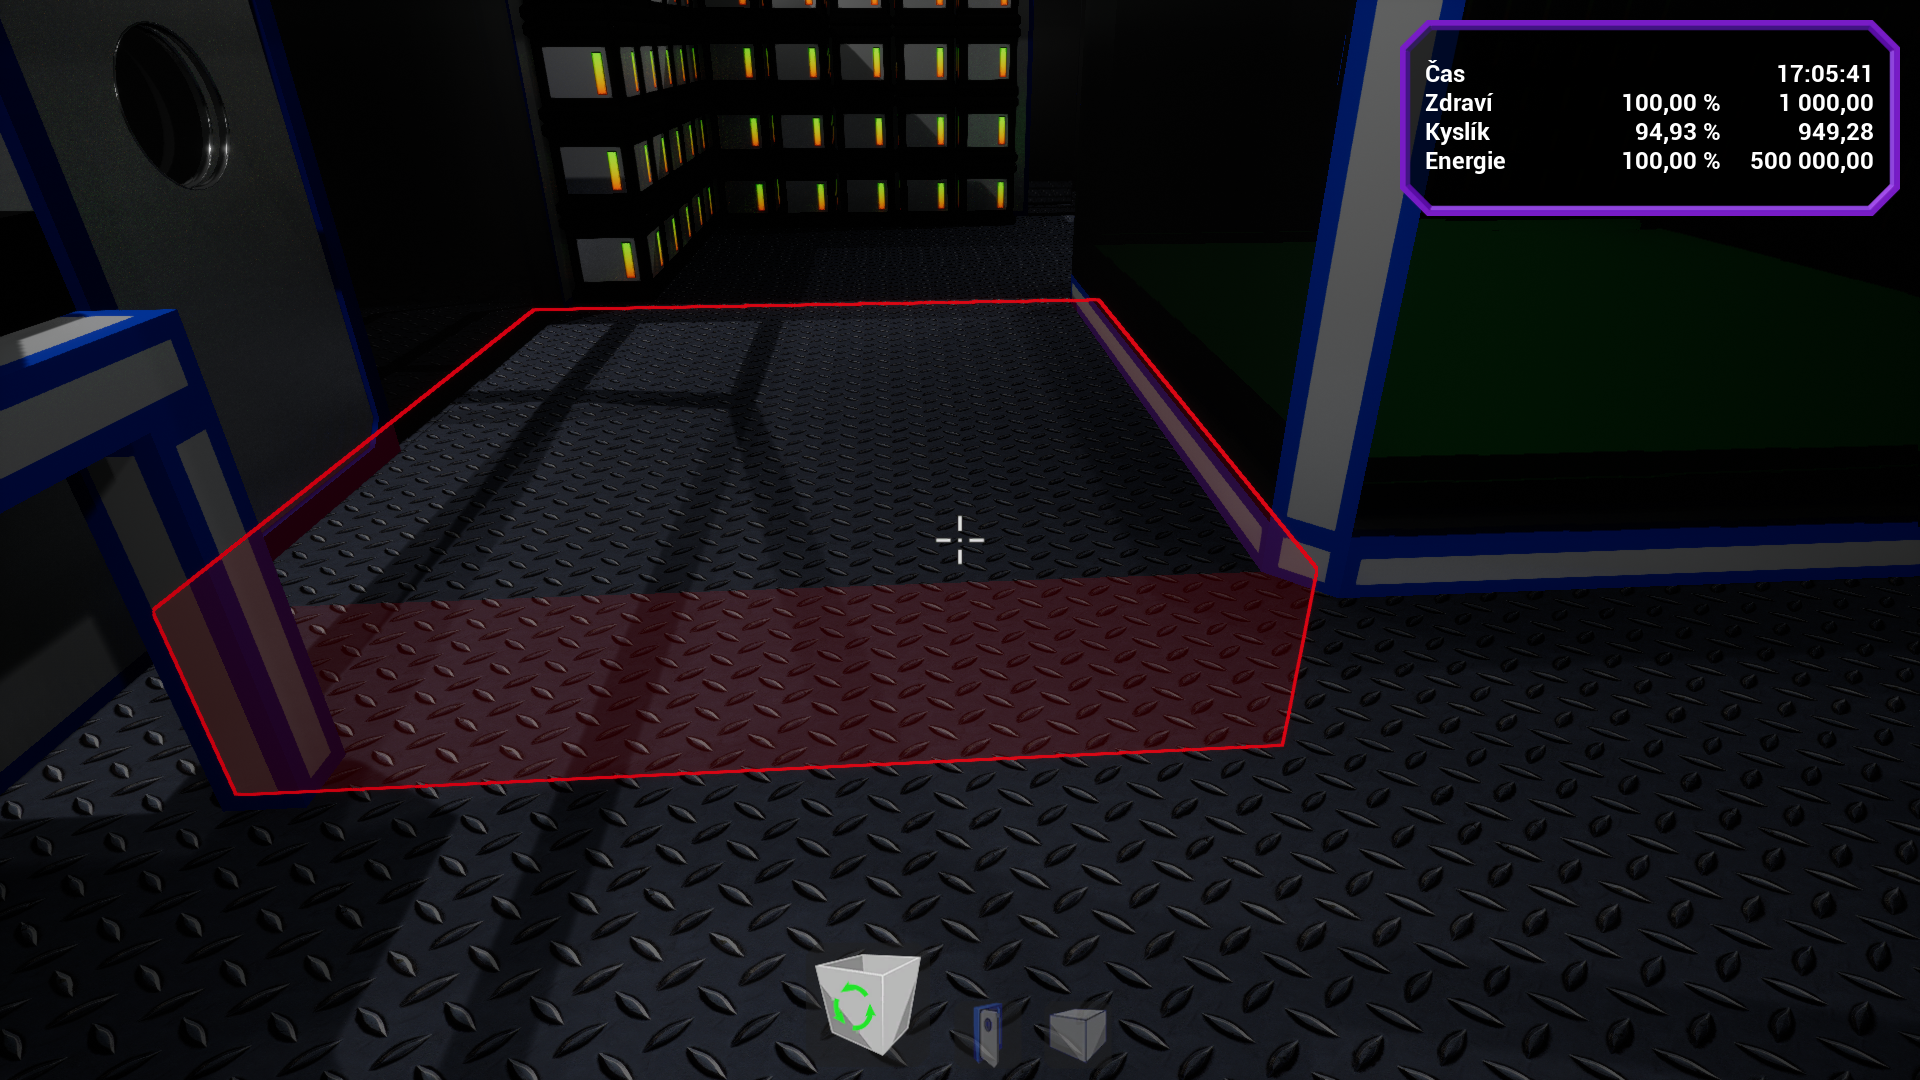
\includegraphics[ width=140mm]{../img/user/buildActions/delete}

\caption{Stavění -- smazat}
\label{fig:user_buildActions_delete}

\end{figure}

\FloatBarrier

Pokud vybereme umístění nového bloku, vidíme žlutě hranice sousedního bloku, ke kterému blok přistavujeme. Stavěný / umisťovaný blok musí mít dostatečné místo pro svoje umístění. Dále je potřeba mít s~sebou dostatečně velkou zásobu energie (dle energetické náročnosti bloku).

\begin{figure}[!ht]\centering
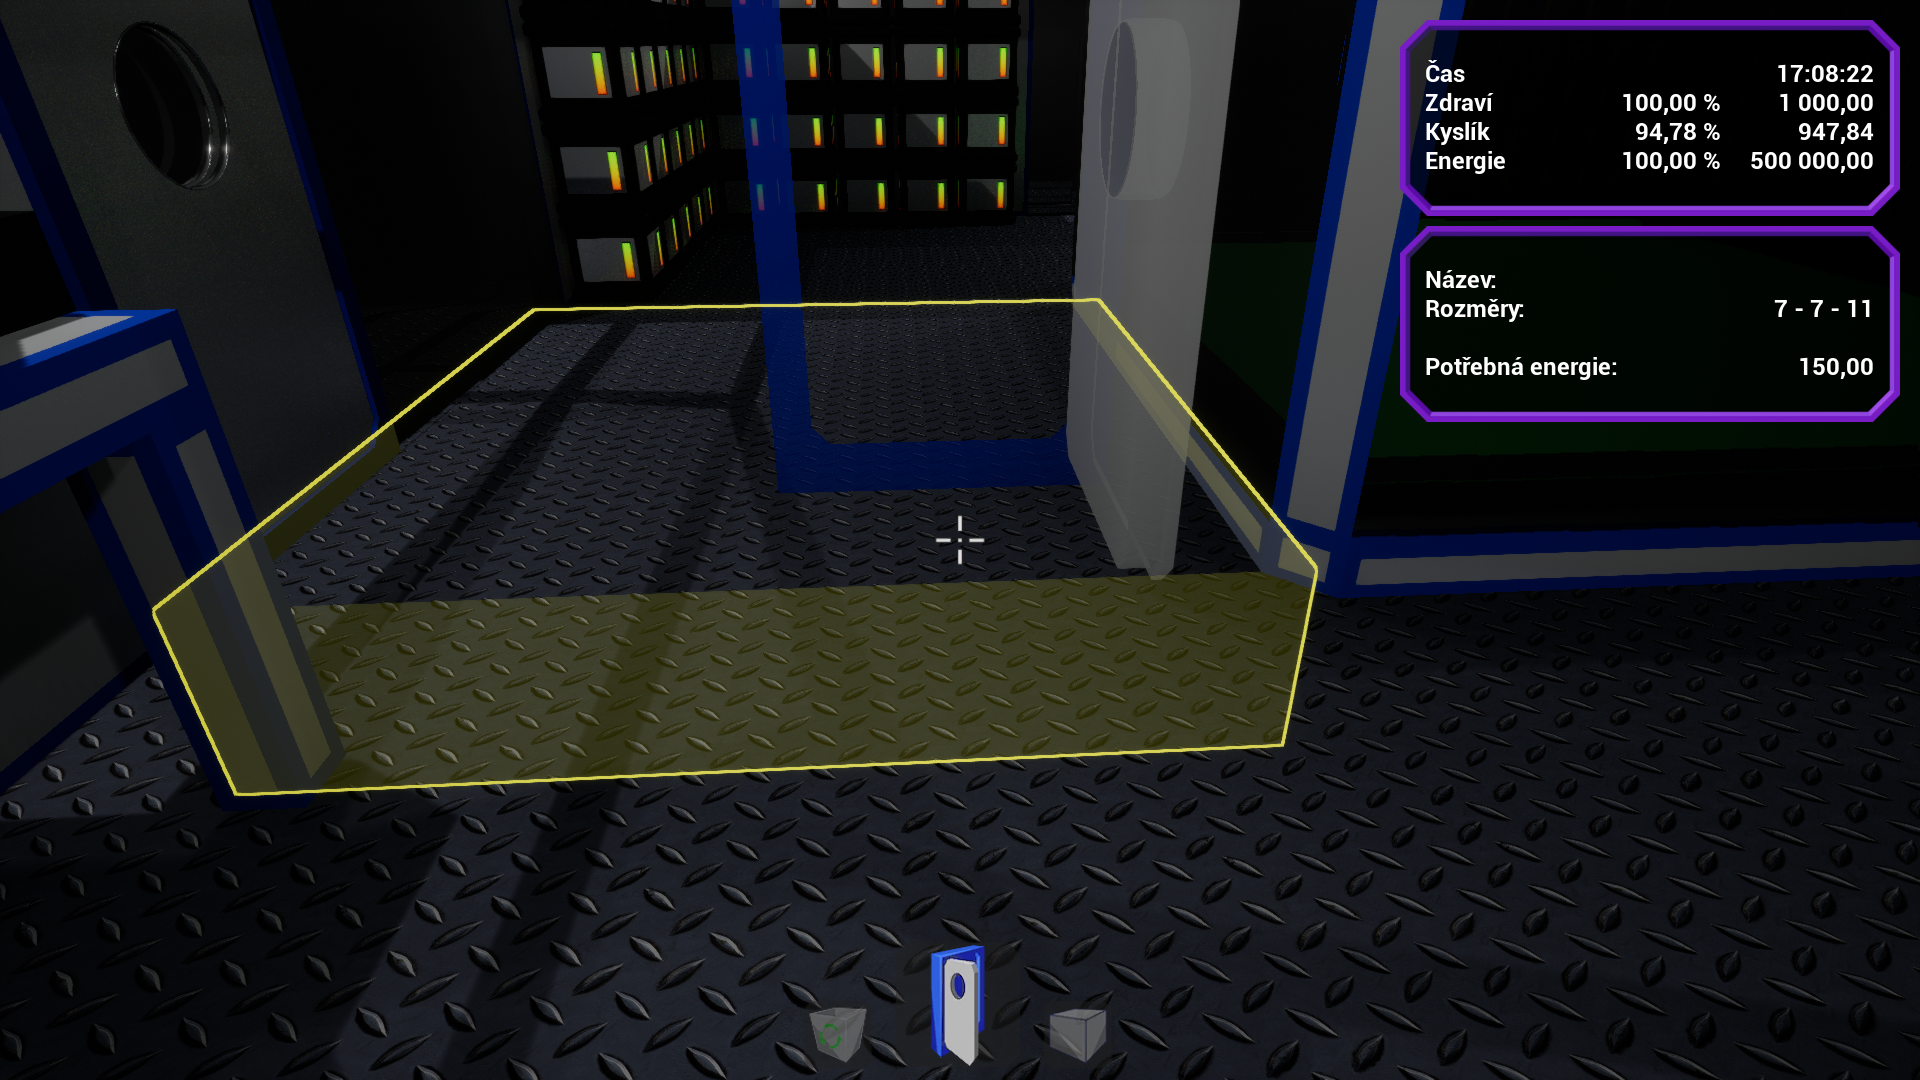
\includegraphics[ width=140mm]{../img/user/buildActions/place}

\caption{Stavění -- umístit}
\label{fig:user_buildActions_place}

\end{figure}

\FloatBarrier

Blok je též možný rotovat (Klávesy v~sekci Insert .. Page Down, případně jejich ekvivalenty 7,8,9,4,5,6).

\begin{figure}[!ht]\centering
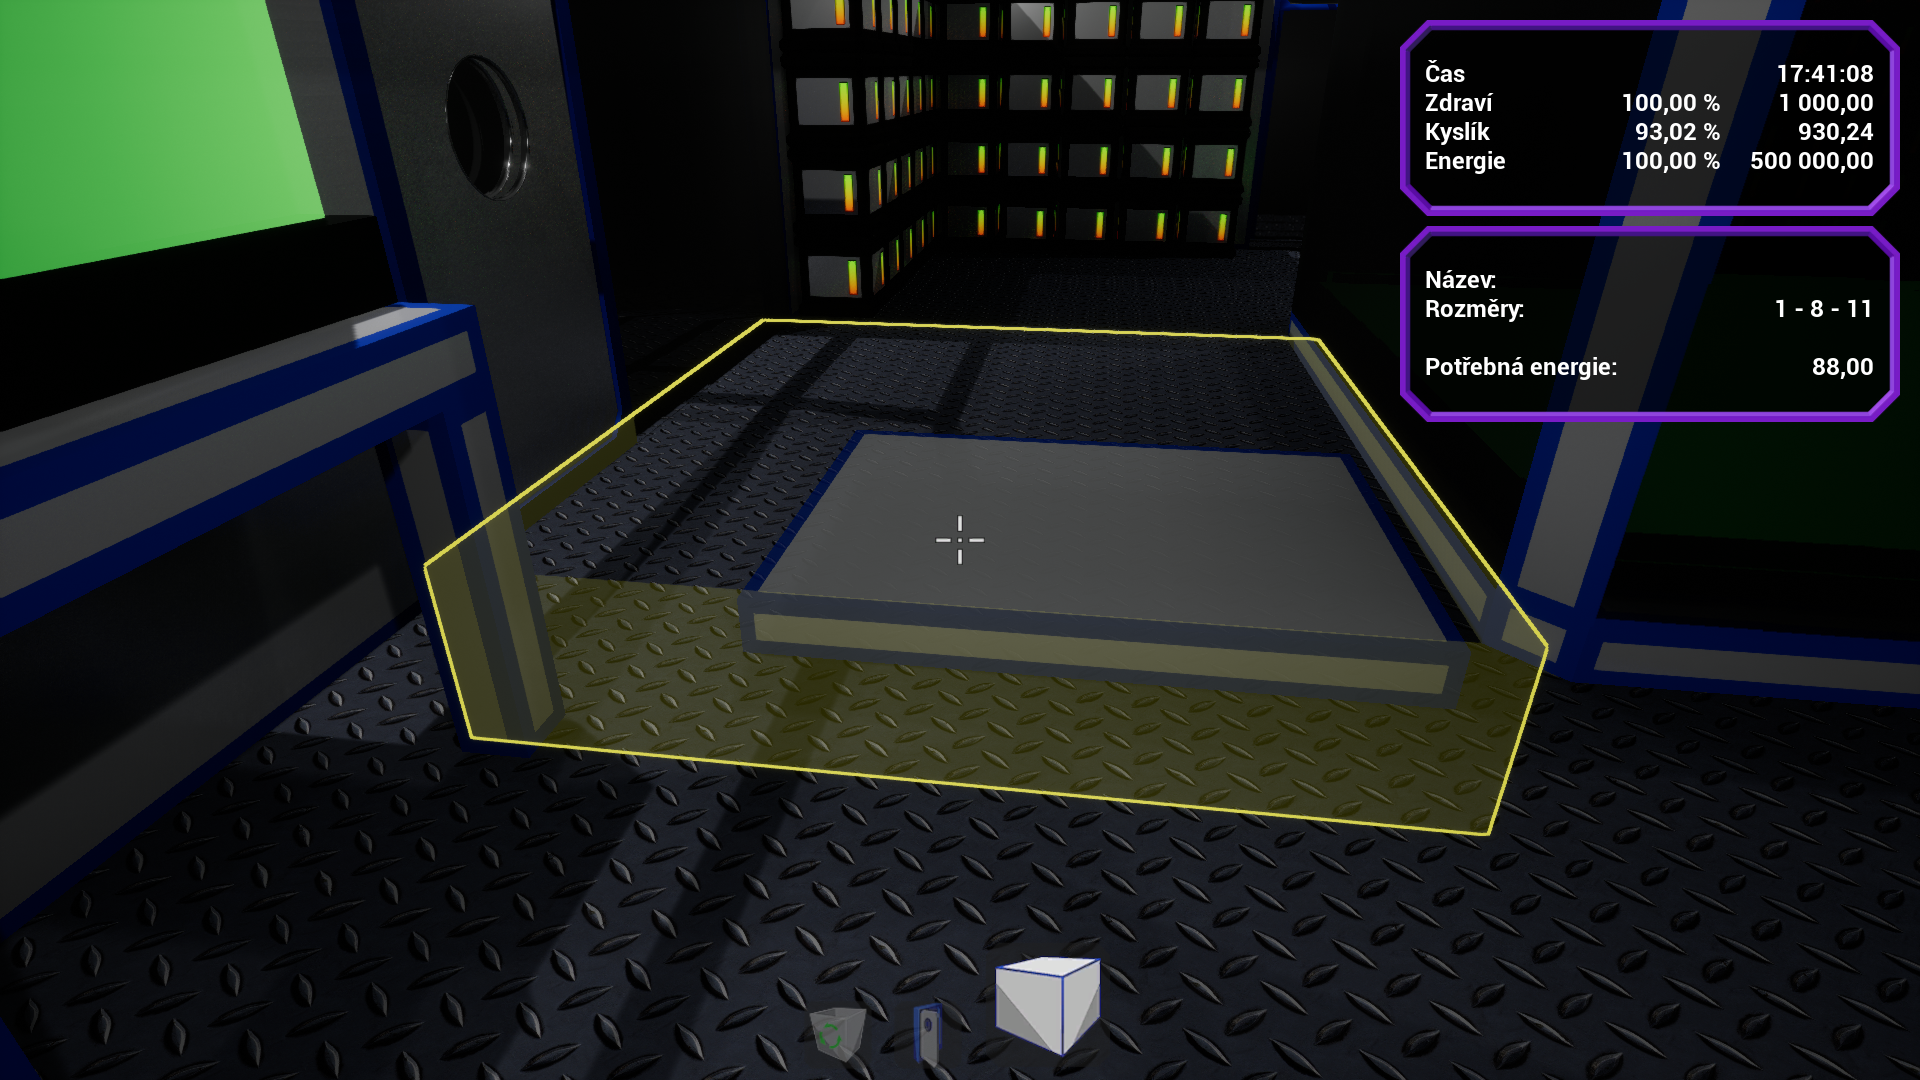
\includegraphics[ width=140mm]{../img/user/buildActions/place_Rotate}

\caption{Stavění -- rotace}
\label{fig:user_buildActions_place_Rotate}

\end{figure}

\FloatBarrier

Pokud bylo umístění v~pořádku, blok již není nadále průhledný a~hráči ubyla energie. Pokud je zapnut kreativní mód, energie samozřejmě neubývá.

\begin{figure}[!ht]\centering
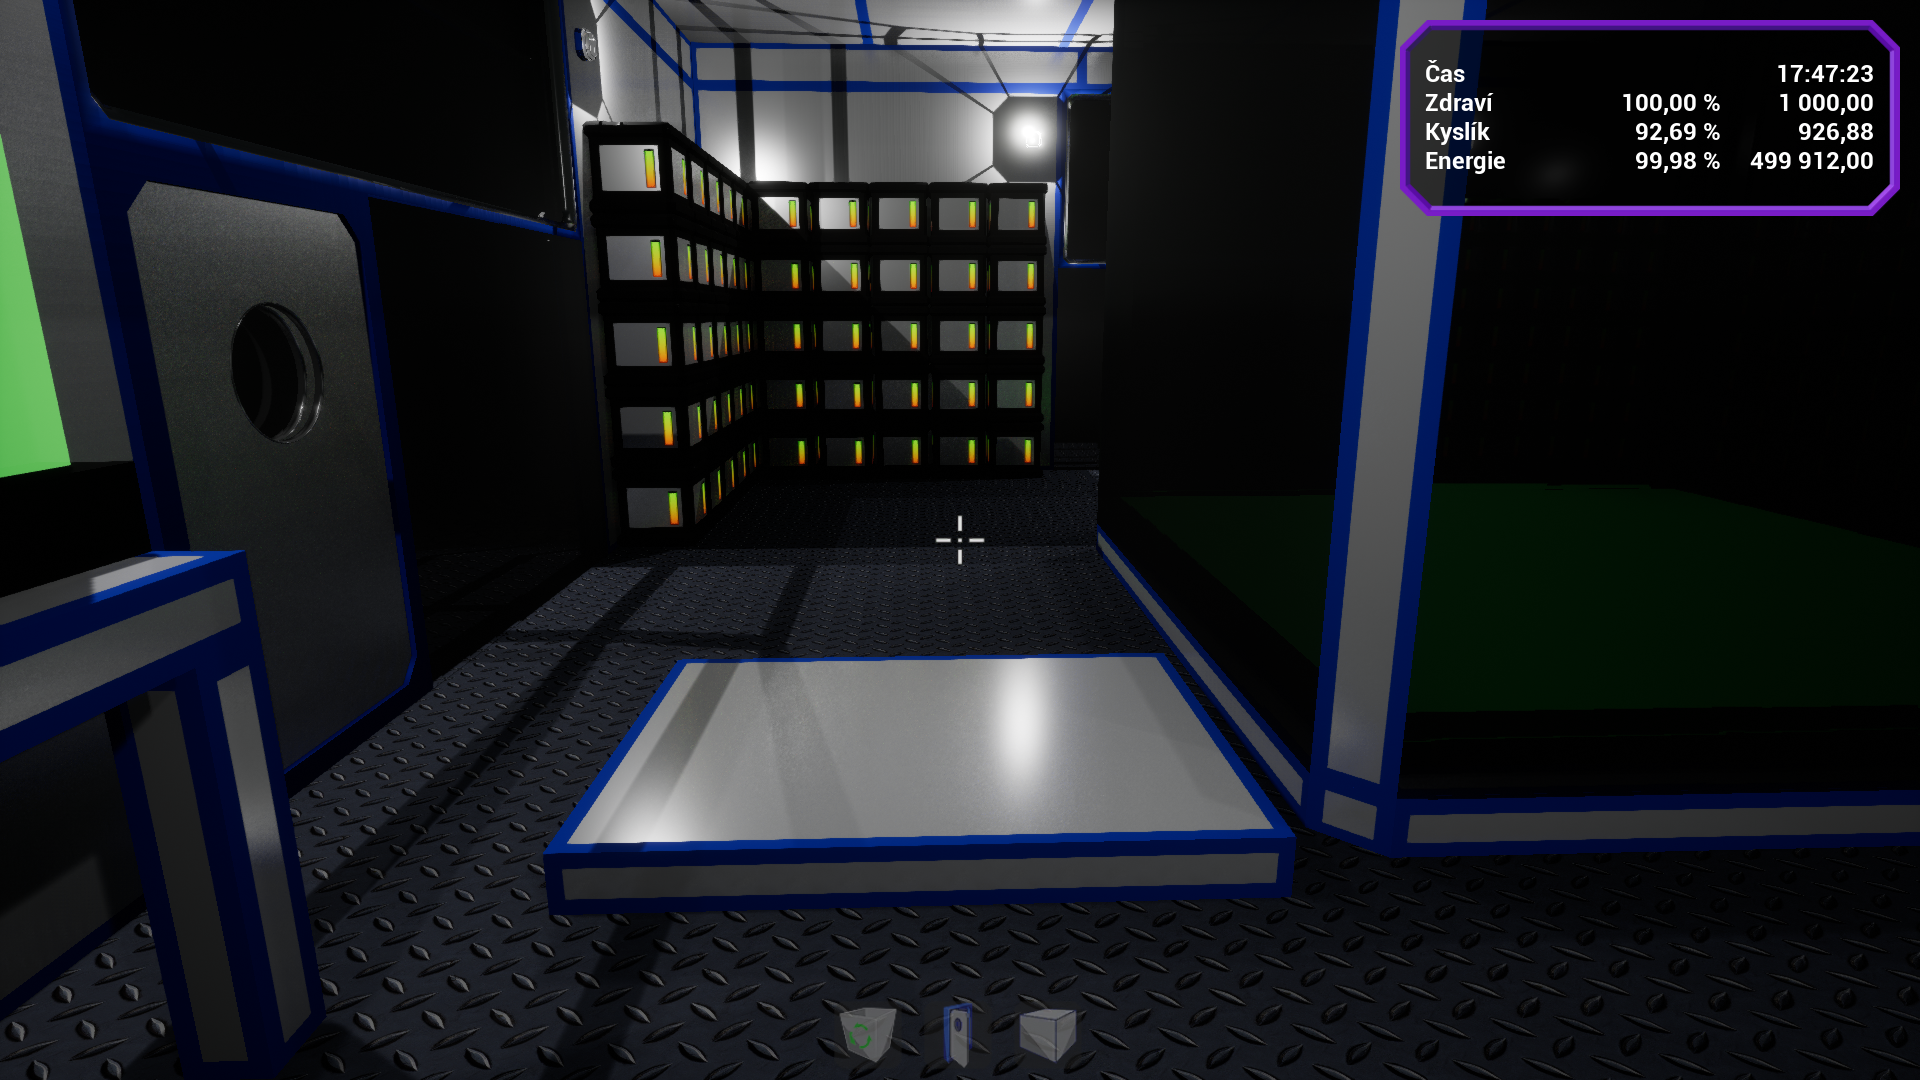
\includegraphics[ width=140mm]{../img/user/buildActions/placeAfter}

\caption{Stavění -- po umístění}
\label{fig:user_buildActions_placeAfter}

\end{figure}


\FloatBarrier
%!TEX root = ../../prace.tex

\section{Umístitelné předměty}

Blok \textbf{Kyslíková bomba} je možné umístit do světa a pak si ho opět vzít do inventáře. Díky tomu je možné tyto bloky dále používat třeba pro plnění v \textbf{Plničce kyslíkových bomb}.
Blok je možné buď rovnou použít (levé tlačítko myši).
Tento blok zároveň rovnou ukazuje, kolik objemu je využito.

\begin{figure}[!ht]\centering
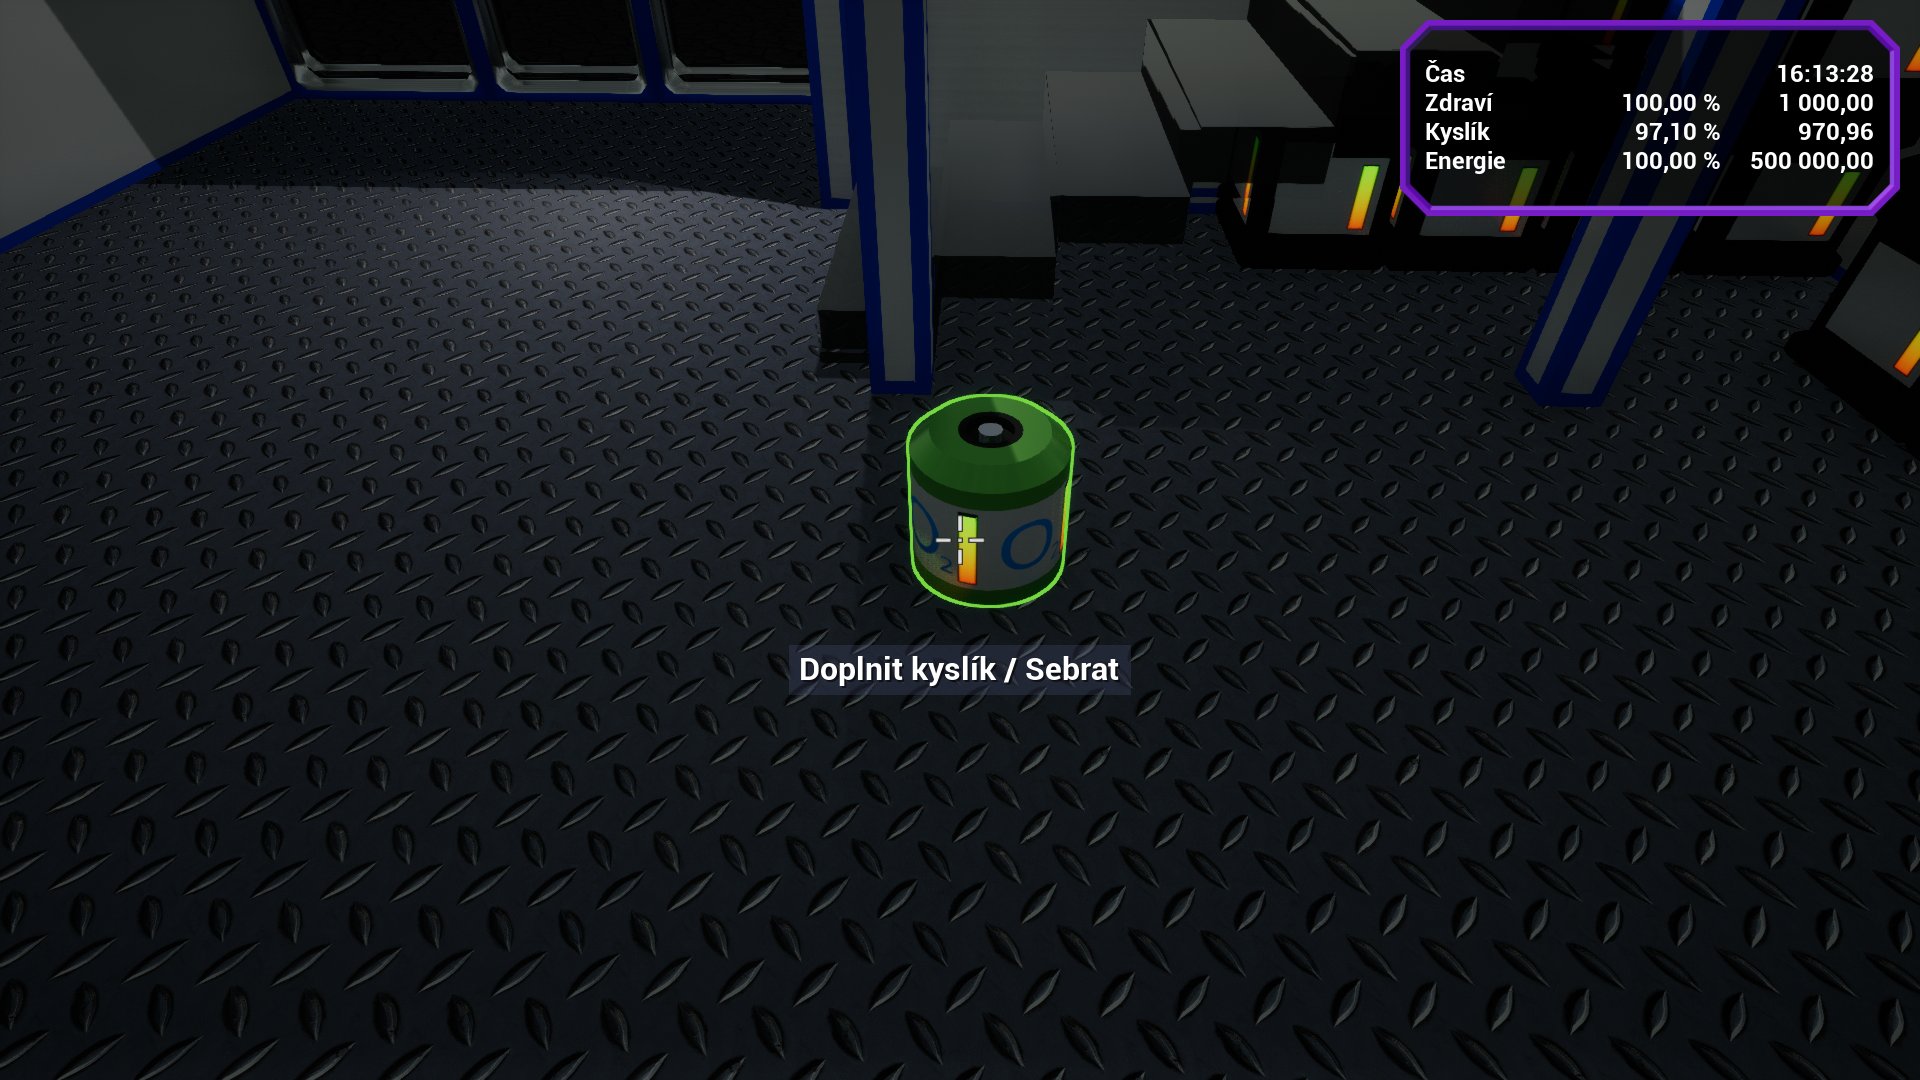
\includegraphics[ width=140mm]{../../img/user/tank/0tankFull}

\caption{Umístitelné předměty - plná kyslíková bomba}
\label{fig:user_tank_0tankFull}

\end{figure}

\FloatBarrier

Na dalším obrázku vidíme již částečně použitou kyslíkovou bombu. Pokud ji pravým tlačítkem myši sebereme a otevřeme si inventář a správnou skupinu (\textbf{Typ: Inventář} v nastavení skupiny), uvidíme tento blok v seznamu.

Požité tagy se při přidání do světa a opětovném sebrání zachovávají.

\begin{figure}[!ht]\centering
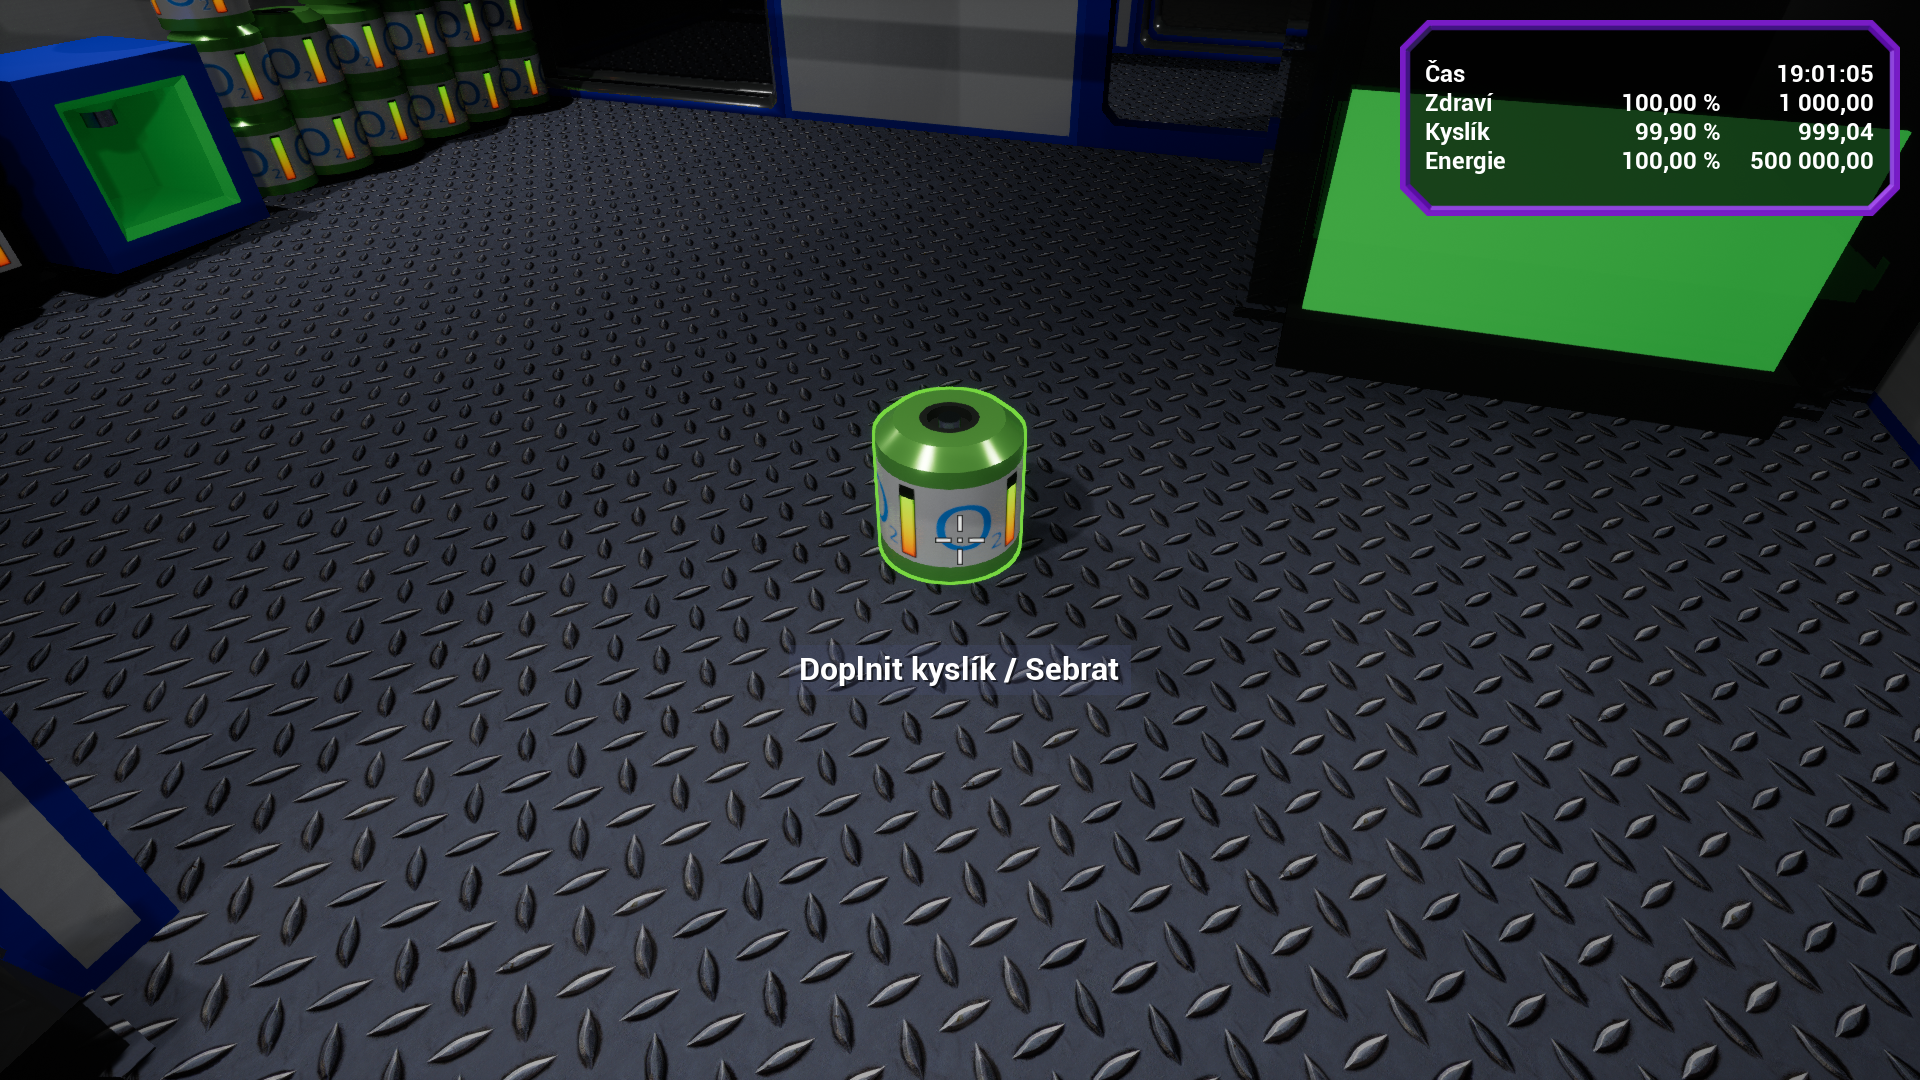
\includegraphics[ width=140mm]{../../img/user/tank/1tankAfterUse}

\caption{Umístitelné předměty - použitá bomba}
\label{fig:user_tank_1tankAfterUse}

\end{figure}

\FloatBarrier

Zároveň v inventáři můžeme vidět přesnou hodnotu naplnění bloku.

\begin{figure}[!ht]\centering
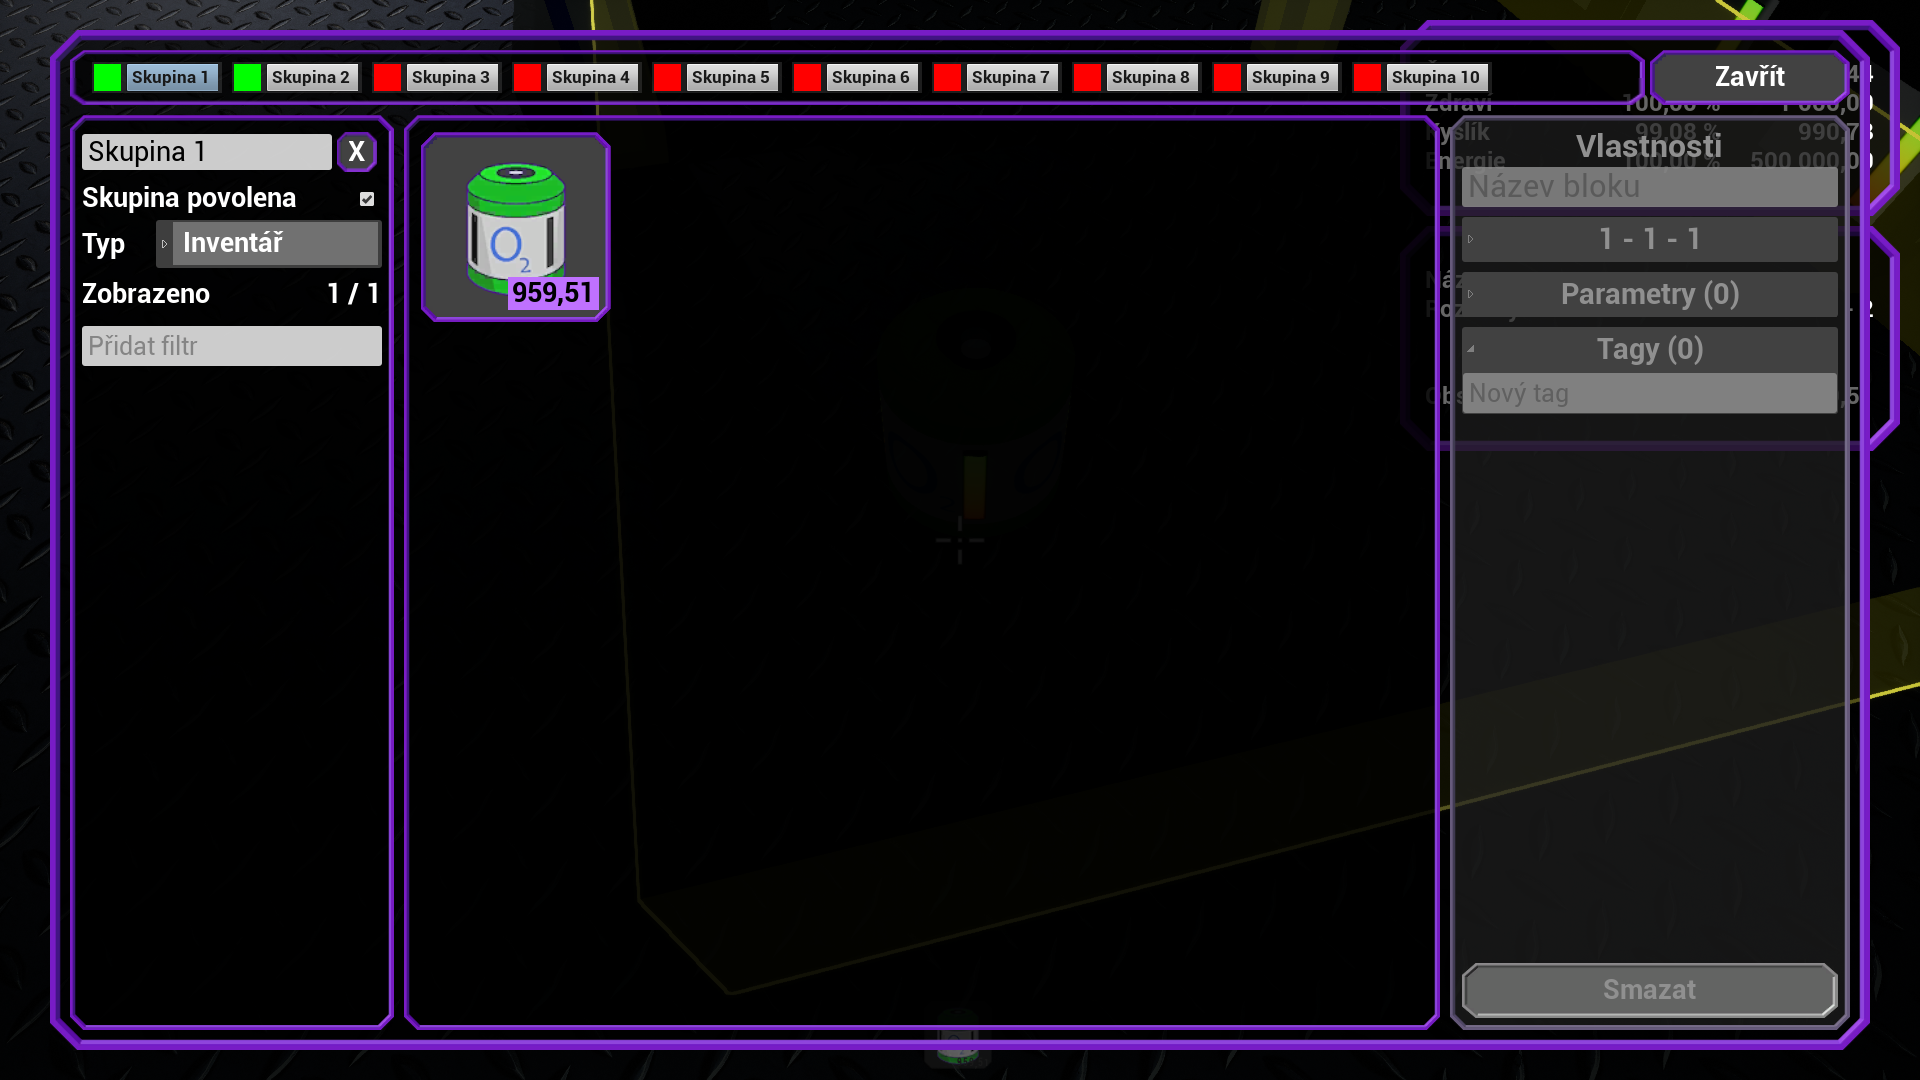
\includegraphics[ width=140mm]{../../img/user/tank/2tankInventory}

\caption{Umístitelné předměty - inventář}
\label{fig:user_tank_2tankInventory}

\end{figure}



\FloatBarrier
%!TEX root = ../../prace.tex

\section{Plnička kyslíkových bomb}

Kyslíkové bomby je potřeba opětovně naplnit, pokud byl jejich obsah spotřebován. Stejně jako u~Kyslíkové bomby, levým tlačítkem myši je možné rovnou doplnit zásoby kyslíku hráče. Pravým se pak otevře ovládací obrazovka.

\begin{figure}[!ht]\centering
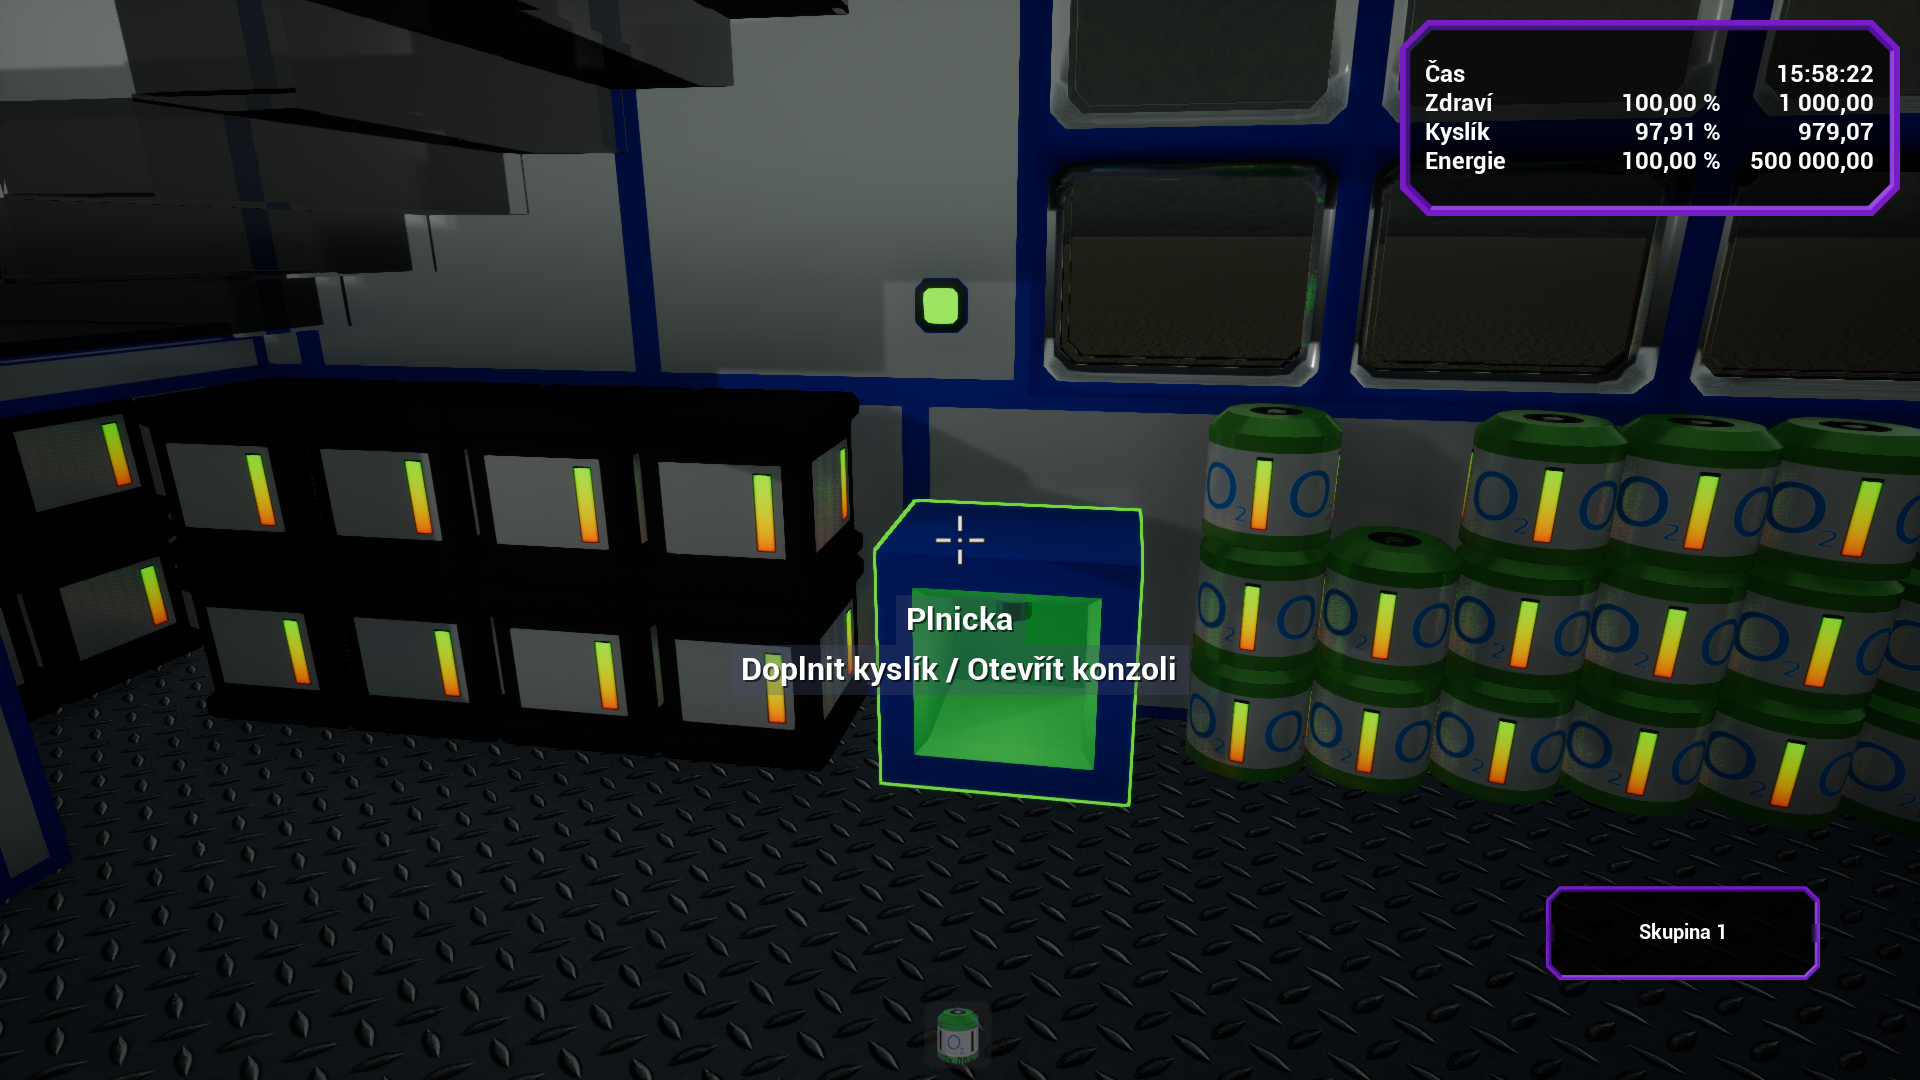
\includegraphics[ width=140mm]{../img/user/filler/0use}

\caption{Plnička kyslíkové bomby -- náhled}
\label{fig:user_filler_0use}

\end{figure}

\FloatBarrier

Ta má v~levé části přiřazený ovladač, případně je možné nejvýše jeden ovladač ze seznamu ovladačů přiřadit. Pokud je přiřazen ovladač, zapnutí bloku se řídí jeho nastavením. V~pravé části je možné regulovat spotřebovávanou energii.

Uprostřed je možné vybrat bomby, které jsou v~inventáři hráče, k~naplnění.

\begin{figure}[!ht]\centering
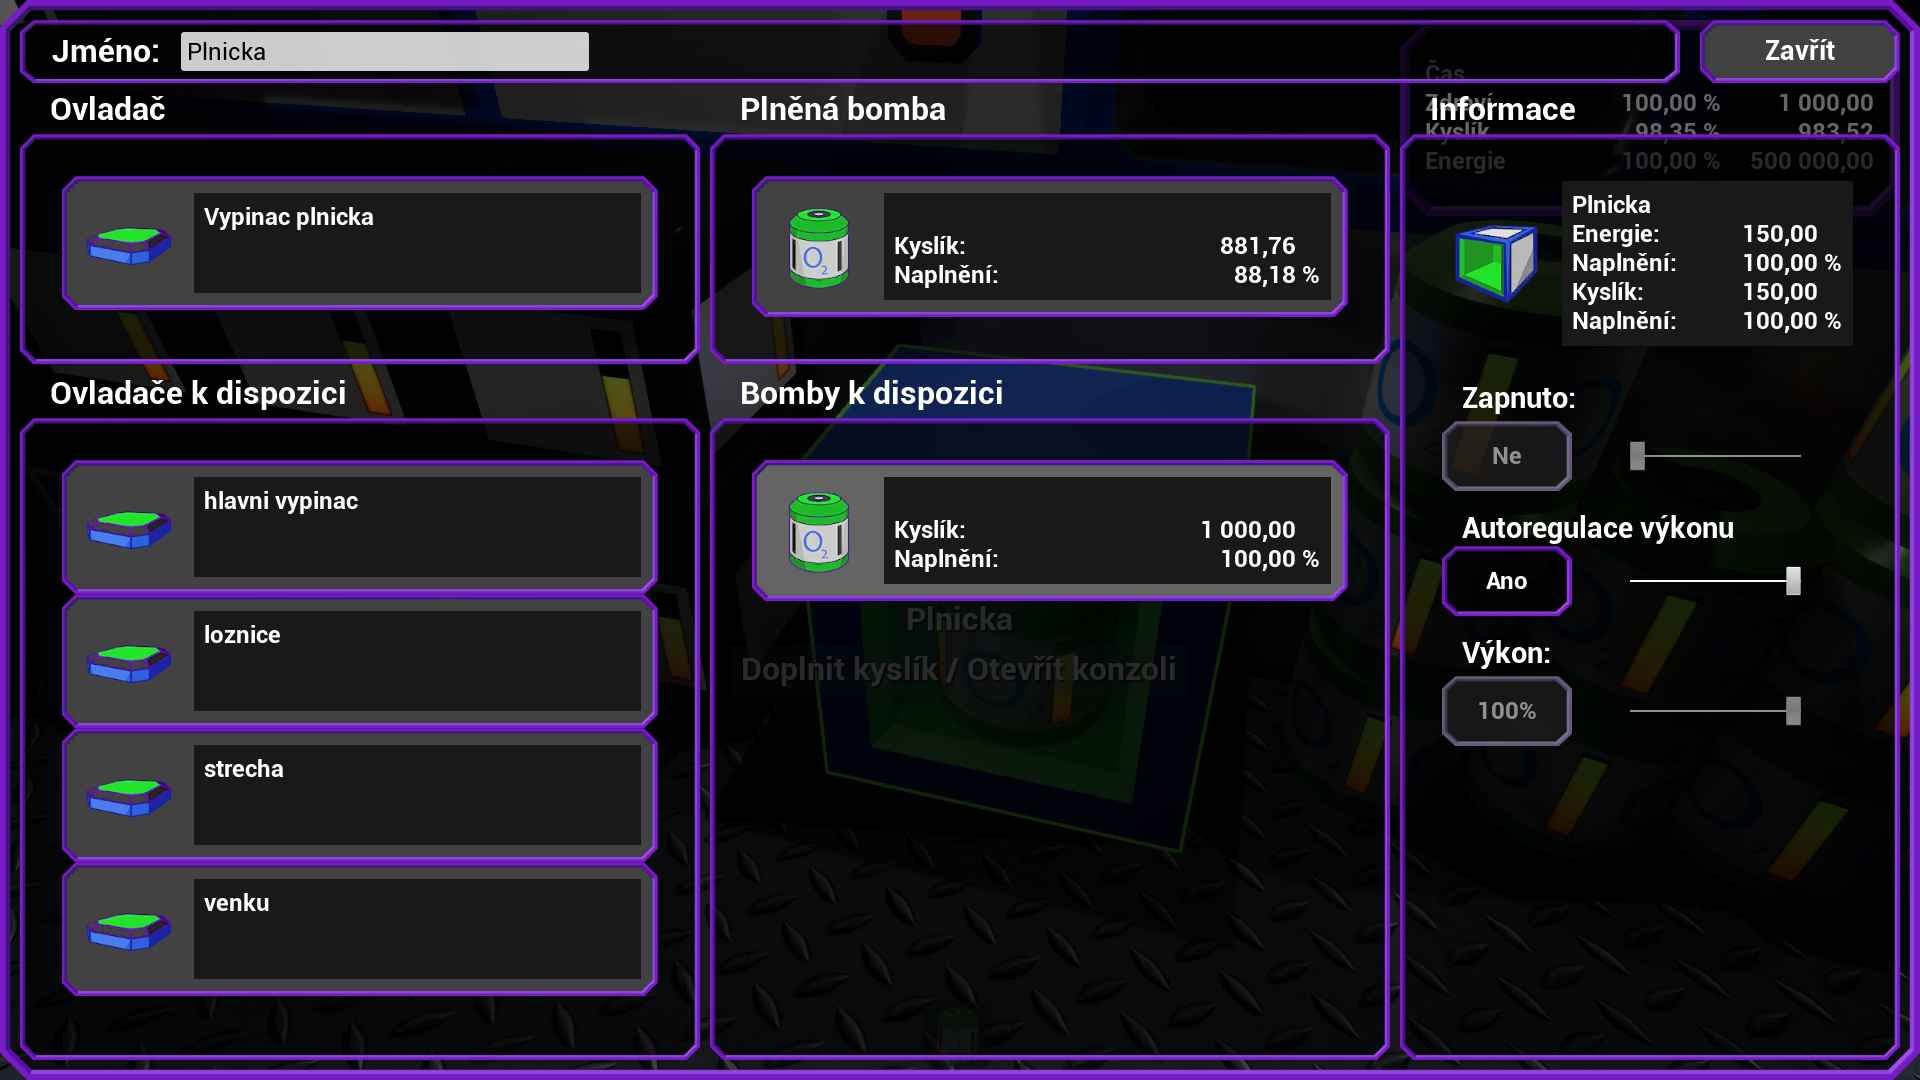
\includegraphics[ width=140mm]{../img/user/filler/1fill}

\caption{Plnička kyslíkové bomby -- ovládací obrazovka}
\label{fig:user_filler_1fill}

\end{figure}

\FloatBarrier

Pokud je plnička zapnuta, generuje kyslík a~ze své zásoby plní přiřazenou kyslíkovou bombu.

\begin{figure}[!ht]\centering
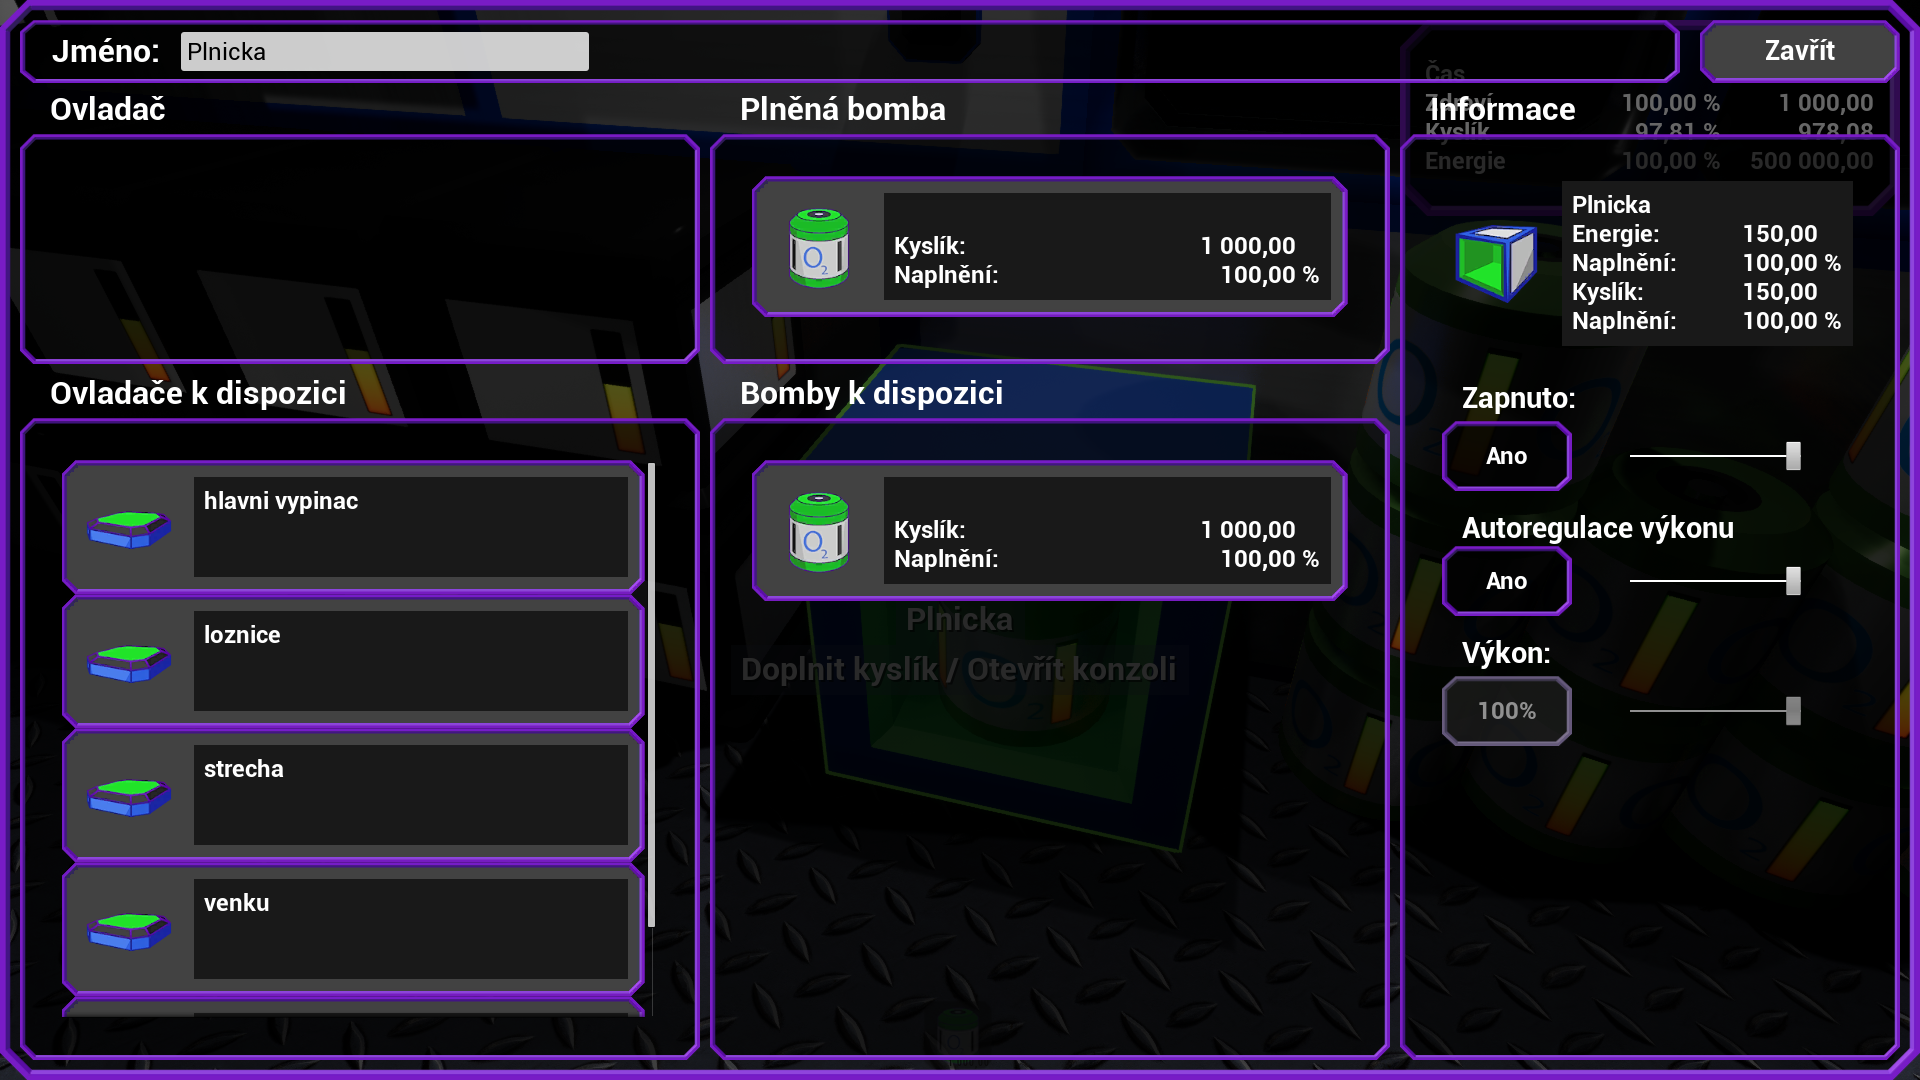
\includegraphics[ width=140mm]{../img/user/filler/2filled}

\caption{Plnička kyslíkové bomby -- naplněno}
\label{fig:user_filler_2filled}

\end{figure}



\FloatBarrier
%!TEX root = ../prace.tex

\section{Přepínač}

Přepínač slouží jako ovládání pro světla a plničku

\begin{figure}[!h]\centering
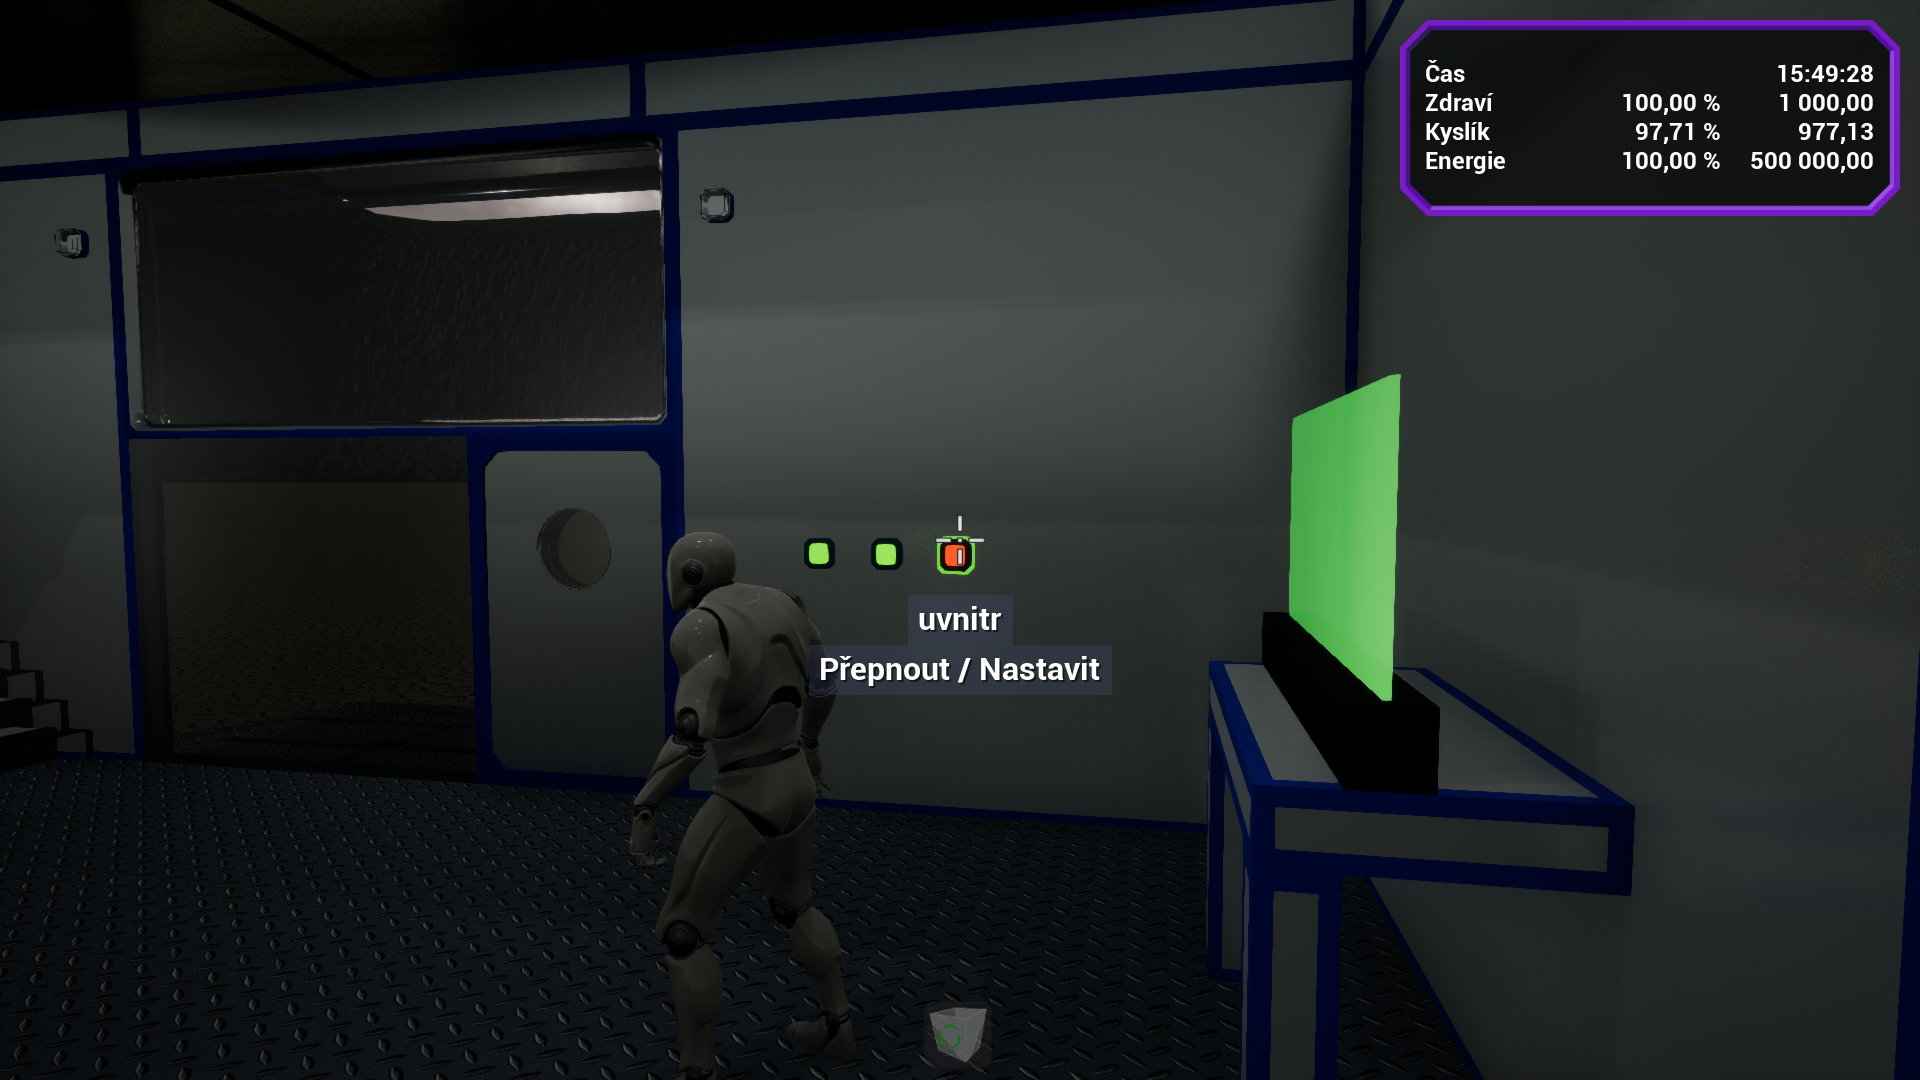
\includegraphics[ width=140mm]{../img/user/switcher/0switcherGeneral}

\caption{Přepínač - den}
\label{fig:user_switcher_0switcherGeneral}

\end{figure}

\FloatBarrier

Blok umožňuje reagovat na denní dobu - automatické přepínání na definovaný stav, pokud začne den, nebo začne noc.

V levé části le možné přiřazovat ovládané bloky

\begin{figure}[!h]\centering
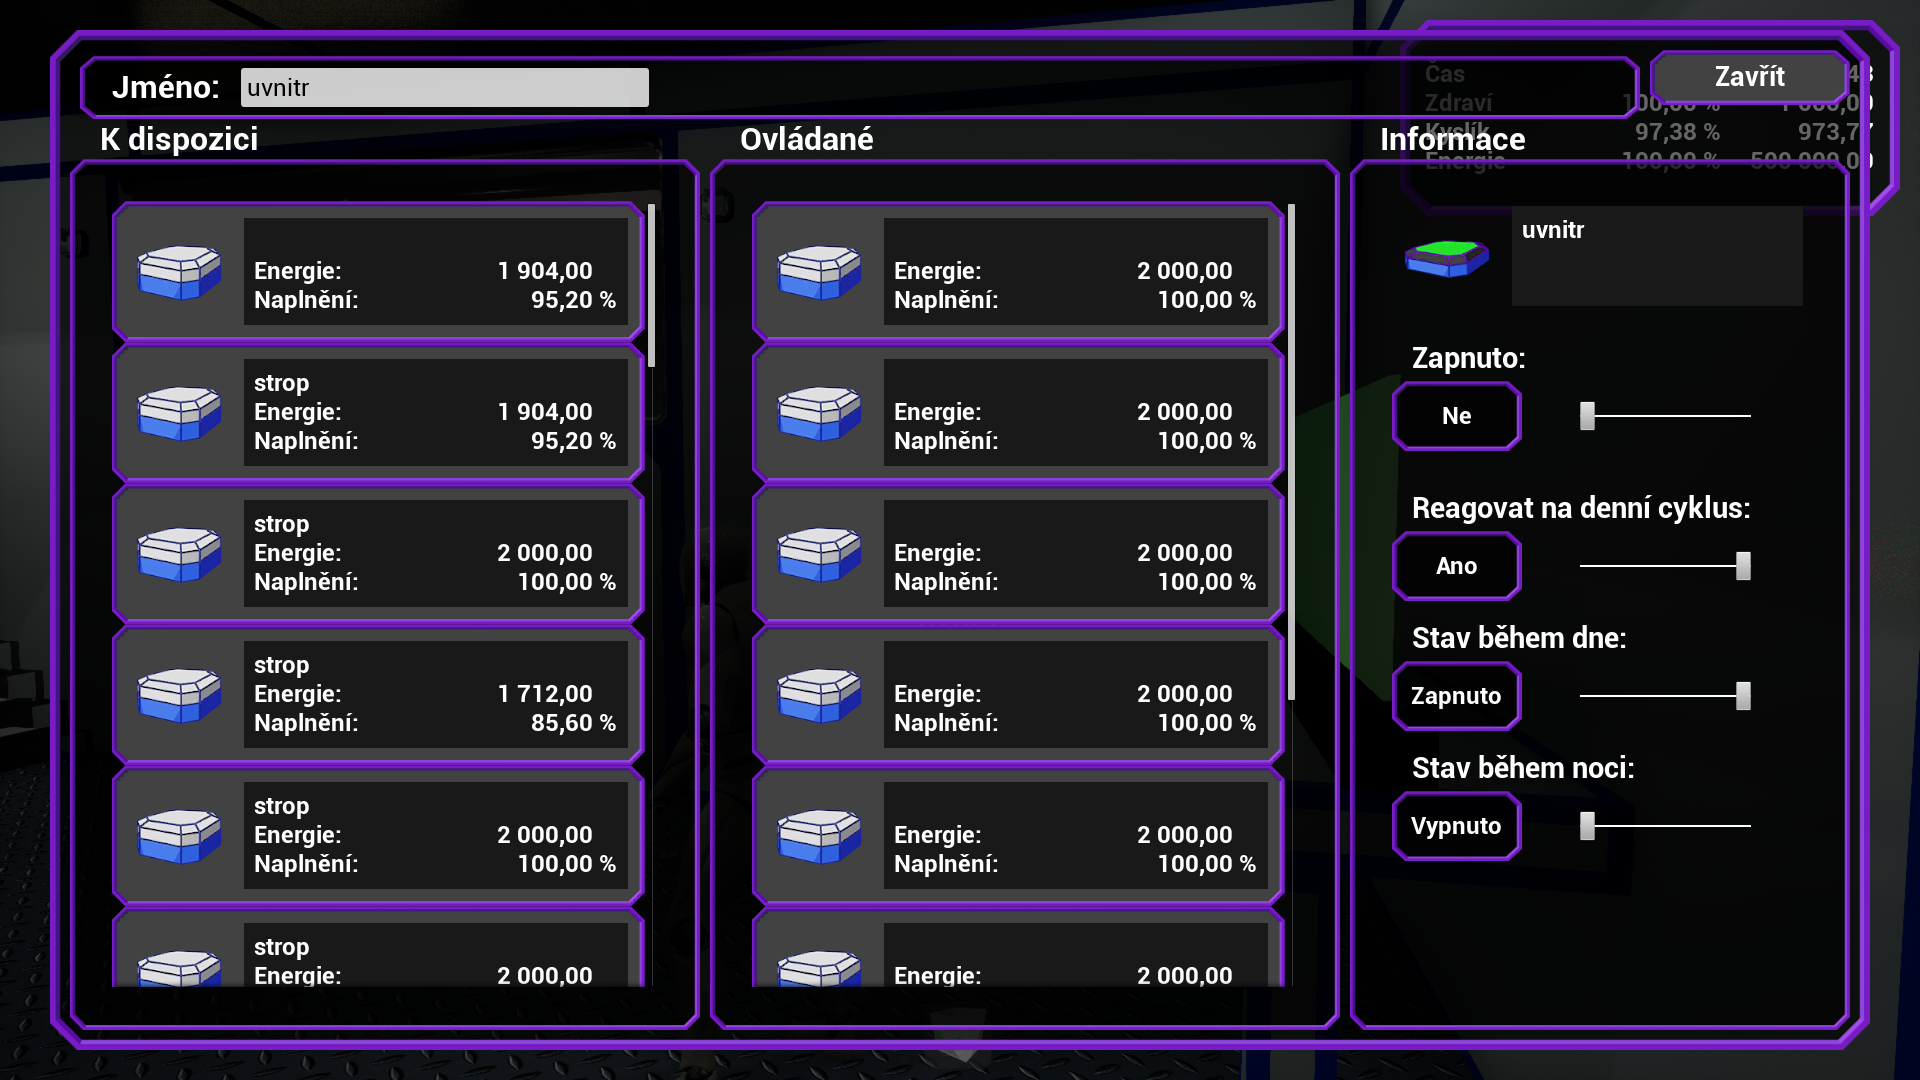
\includegraphics[ width=140mm]{../img/user/switcher/switcherControls}

\caption{Přepínač - poledne, zataženo}
\label{fig:user_switcher_switcherControls}

\end{figure}


\FloatBarrier
%!TEX root = ../prace.tex

\section{Světlo}

Světlo má podobné rozhraní jako Plnička. V levé části se přiřazuje ovladač, v pravé se edituje výkon bloku.

\begin{figure}[!ht]\centering
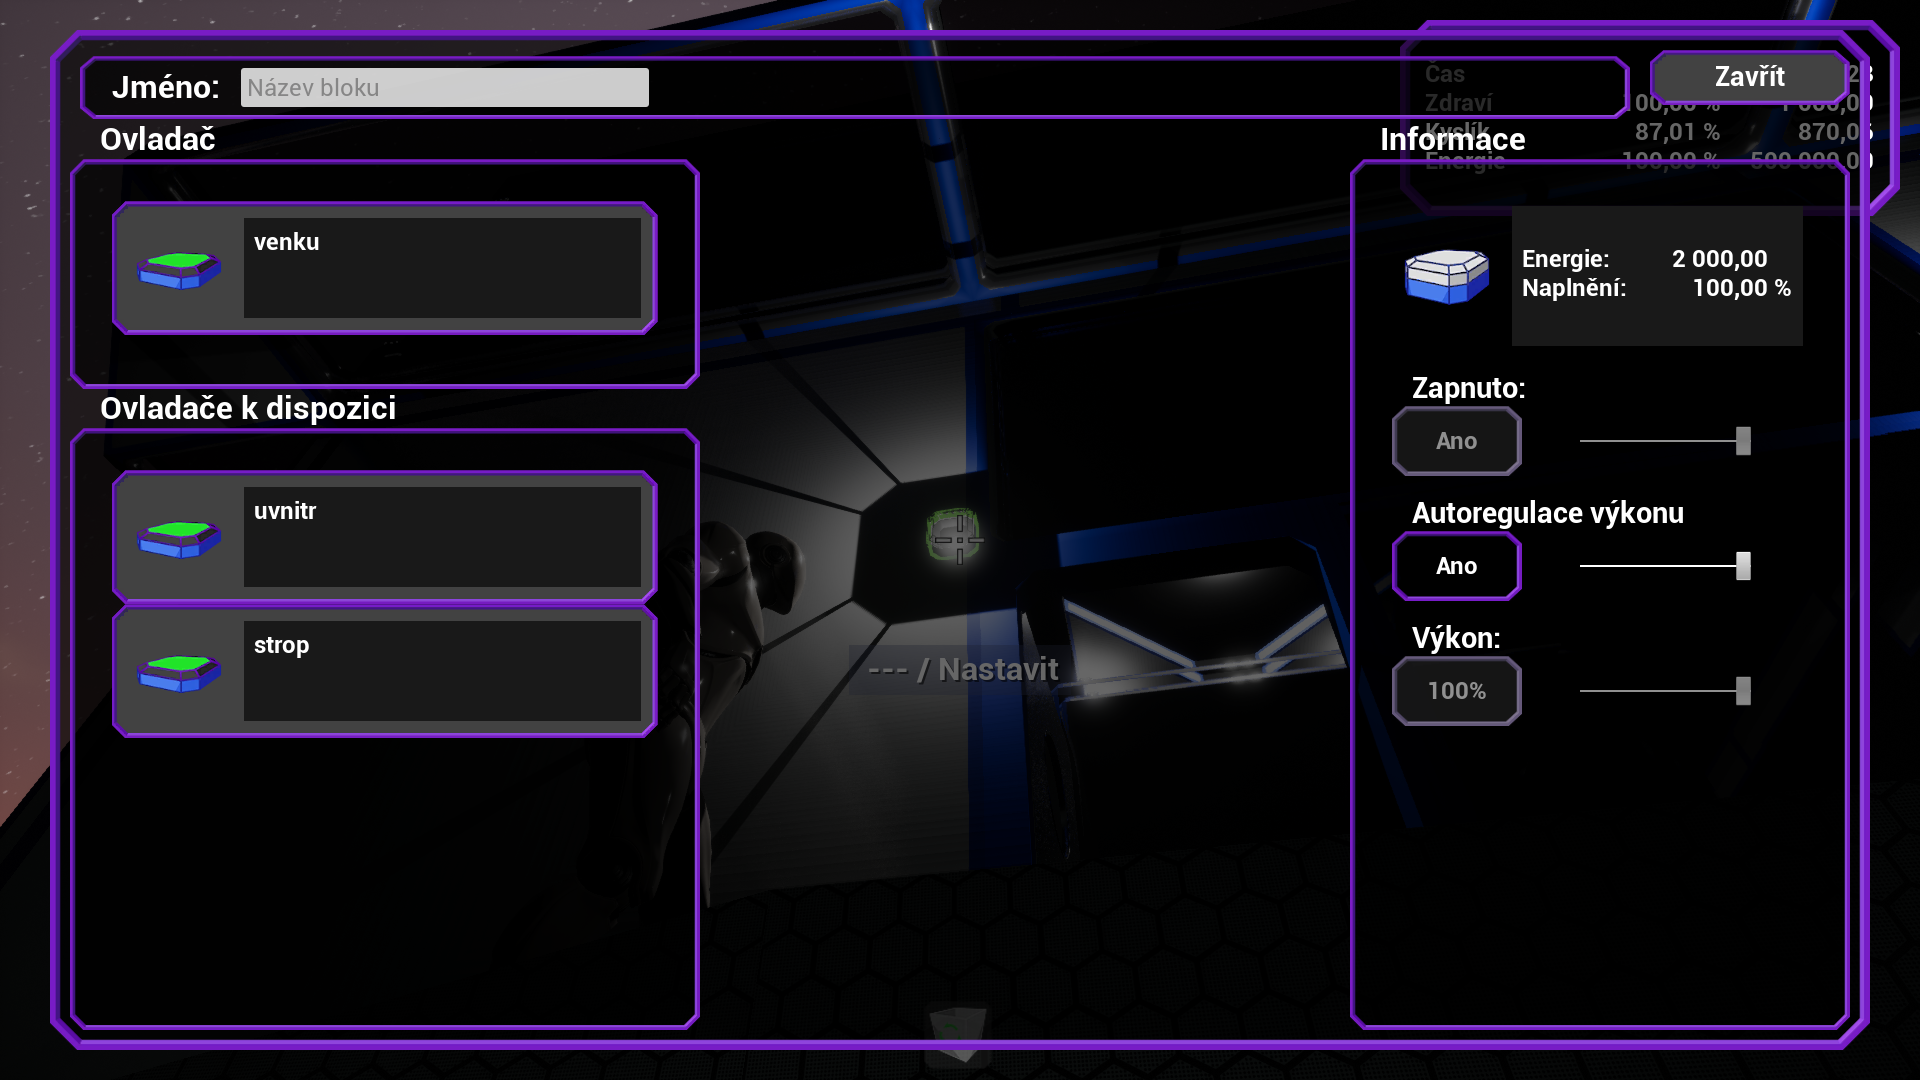
\includegraphics[ width=140mm]{../img/user/light/0light}

\caption{Světlo - ovládací obrazovka}
\label{fig:user_light_0light}

\end{figure}

\FloatBarrier

%!TEX root = ../prace.tex

\section{Kyselý déšť}

Pokud se blíží bouře kyselého deště, nebo právě jedna probíhá, hráč vidí v levé horní části obrazovky zprávu s odhadovaným časem a intenzitou.

To umožňuje strategicky řídit chod svých budov a případně limitovat spotřebovávané zdroje v případě očekávaných dlouhotrvajících bouří. Odhadovaný čas je udán v herním čase.

\begin{figure}[!ht]\centering
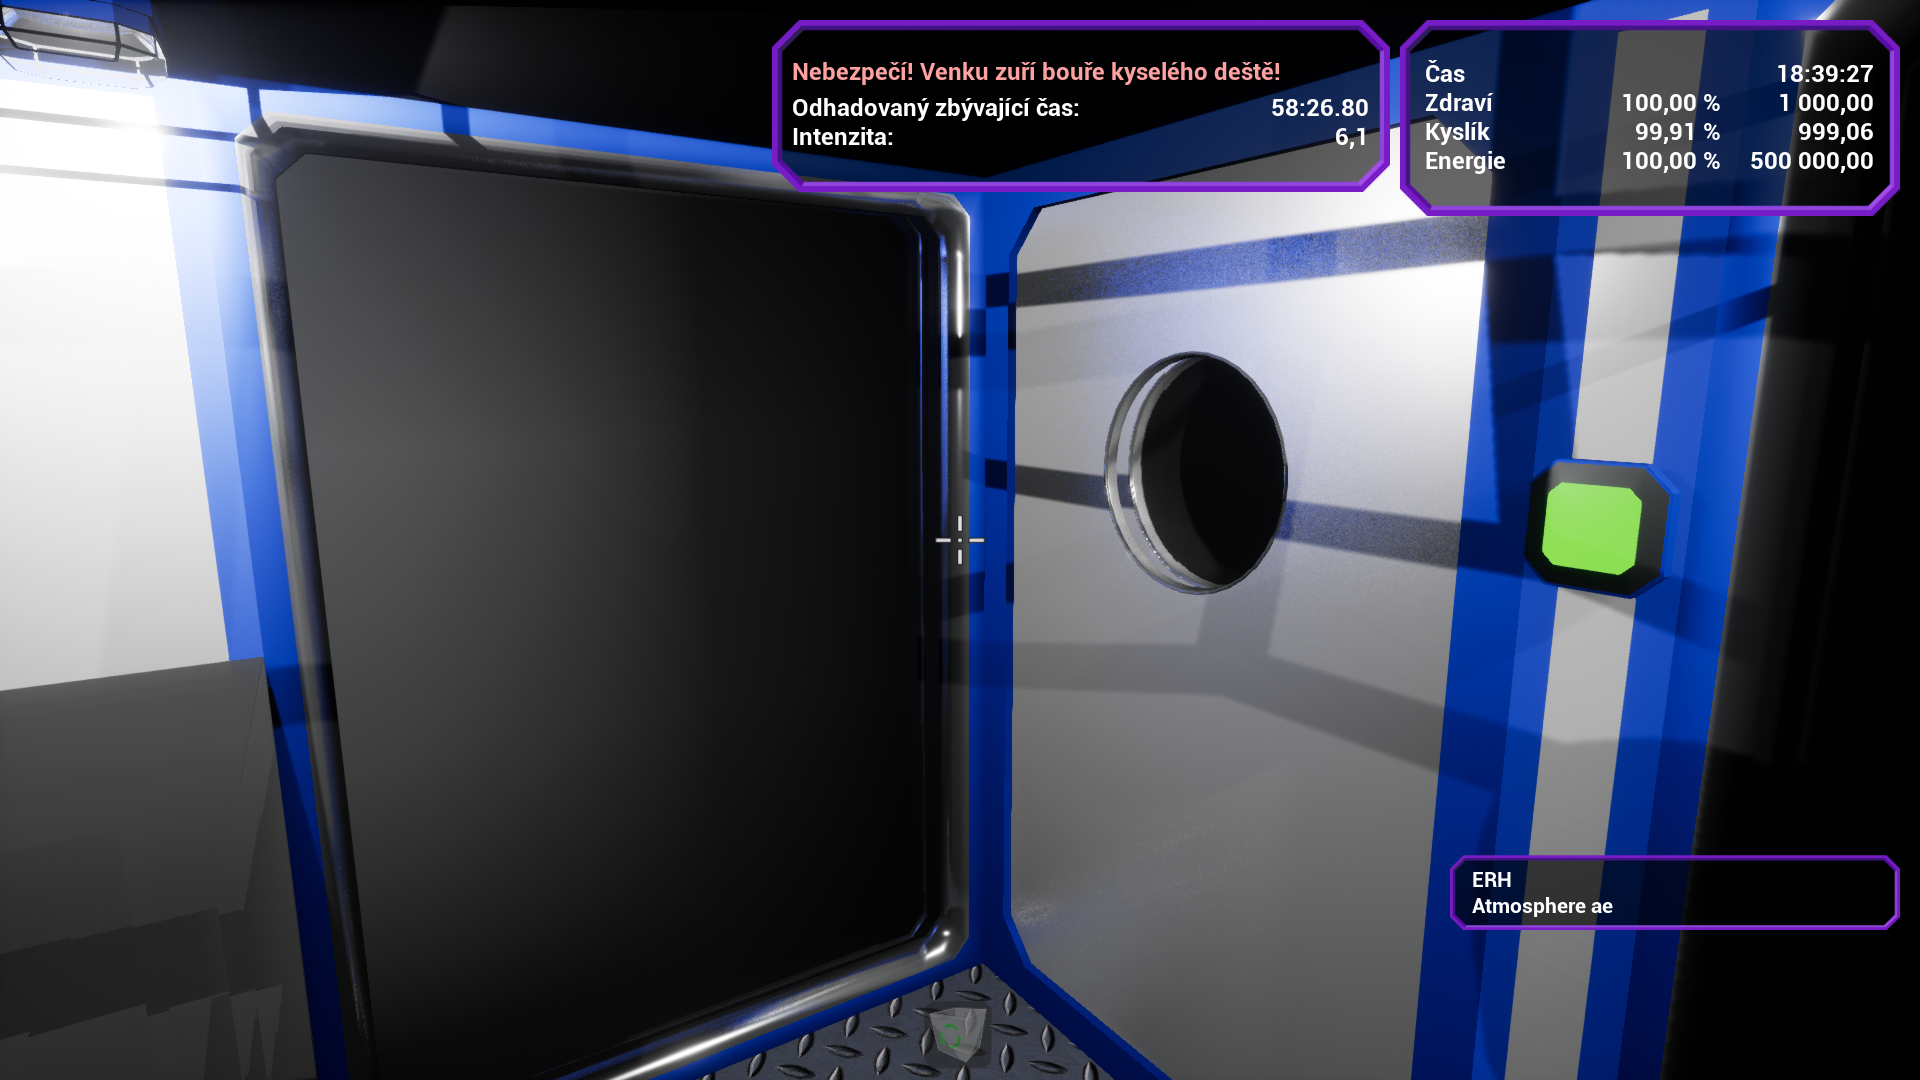
\includegraphics[ width=140mm]{../img/user/rain/0rainInfo}

\caption{Kyselý déšť - info}
\label{fig:user_rain_0rainInfo}

\end{figure}

\FloatBarrier

Pokud hráč není ukrytý v budově či pod nějakým blokem, dostává zásahy. Dokud má dostatek energie, je schopen odolávat účinkům bouře, v momentě, kdy mu energie dojde, začne mu ubývat zdraví.


\begin{figure}[!ht]\centering
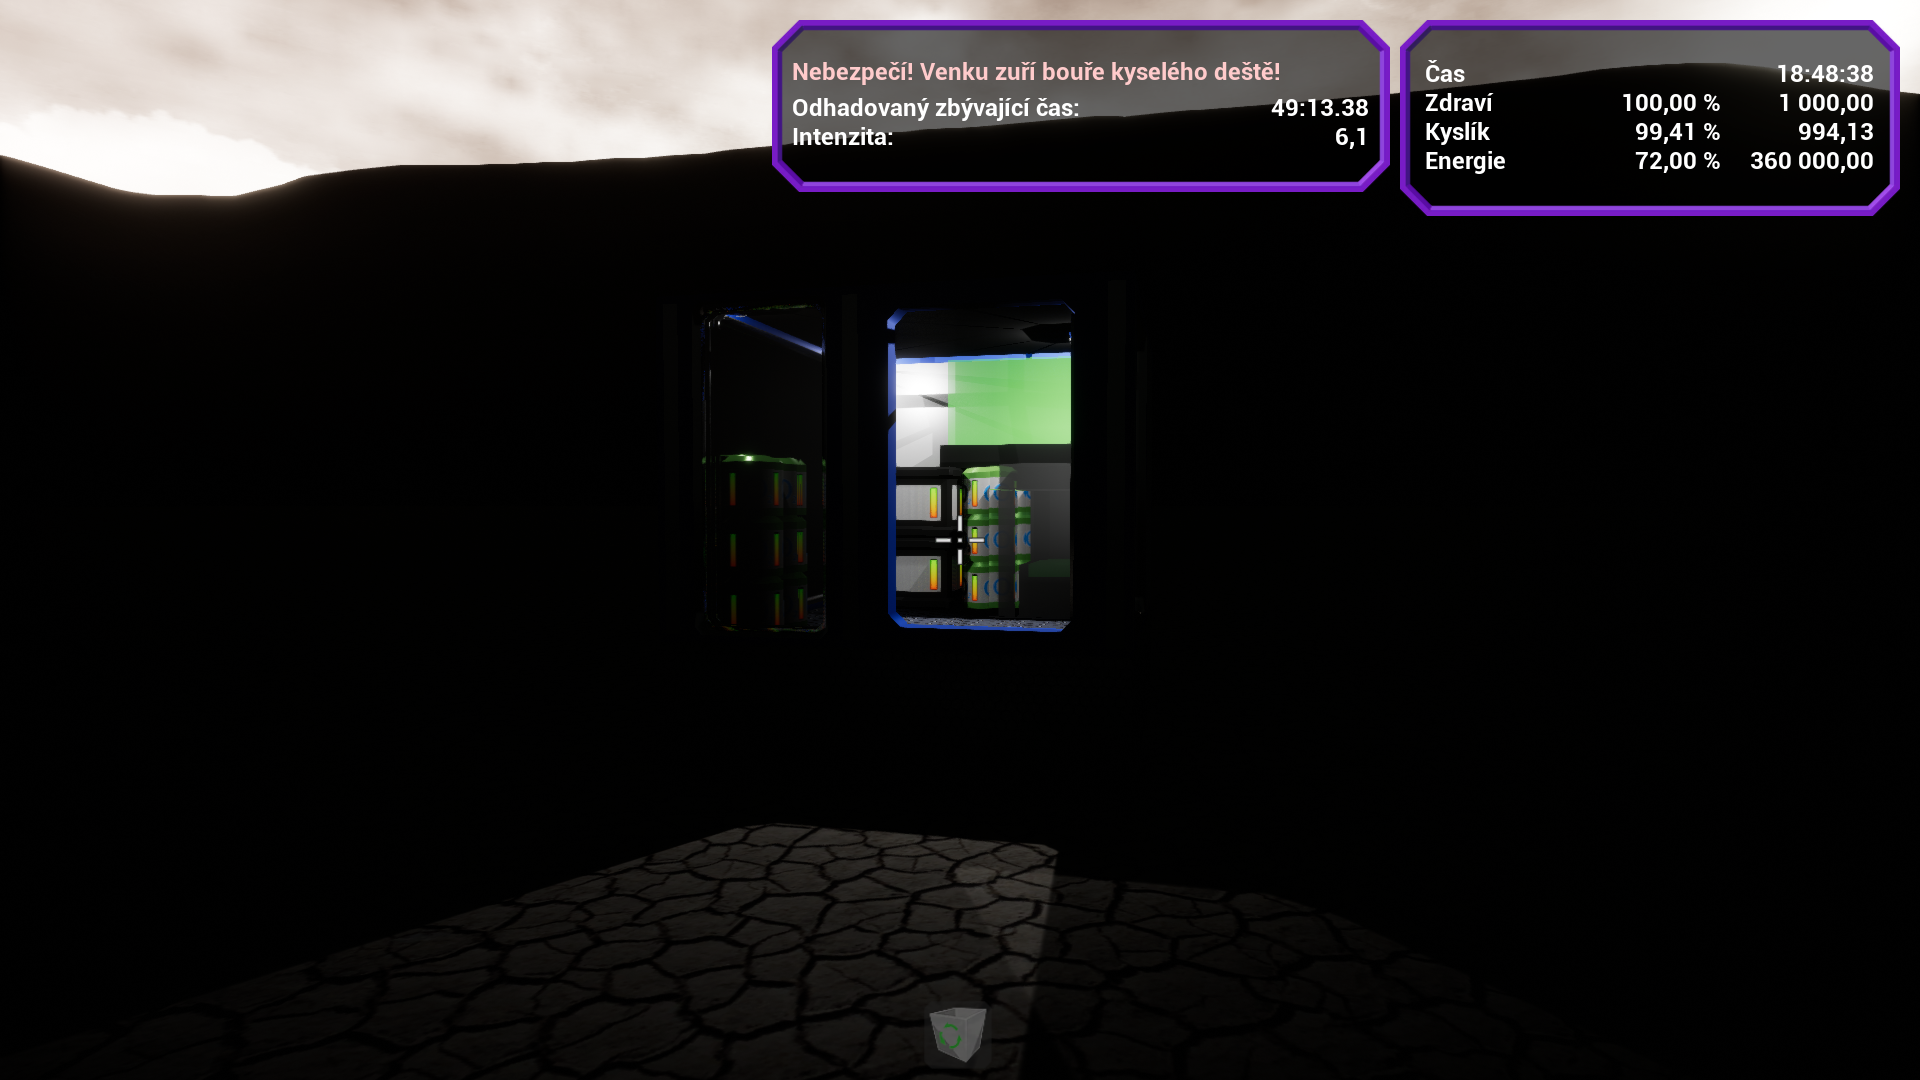
\includegraphics[ width=140mm]{../img/user/rain/1rainDamage}

\caption{Kyselý déšť - zásahy}
\label{fig:user_rain_1rainDamage}

\end{figure}

\FloatBarrier

Pokud si hráč doplní energii, začne se mu zdraví obnovovat.

\begin{figure}[!ht]\centering
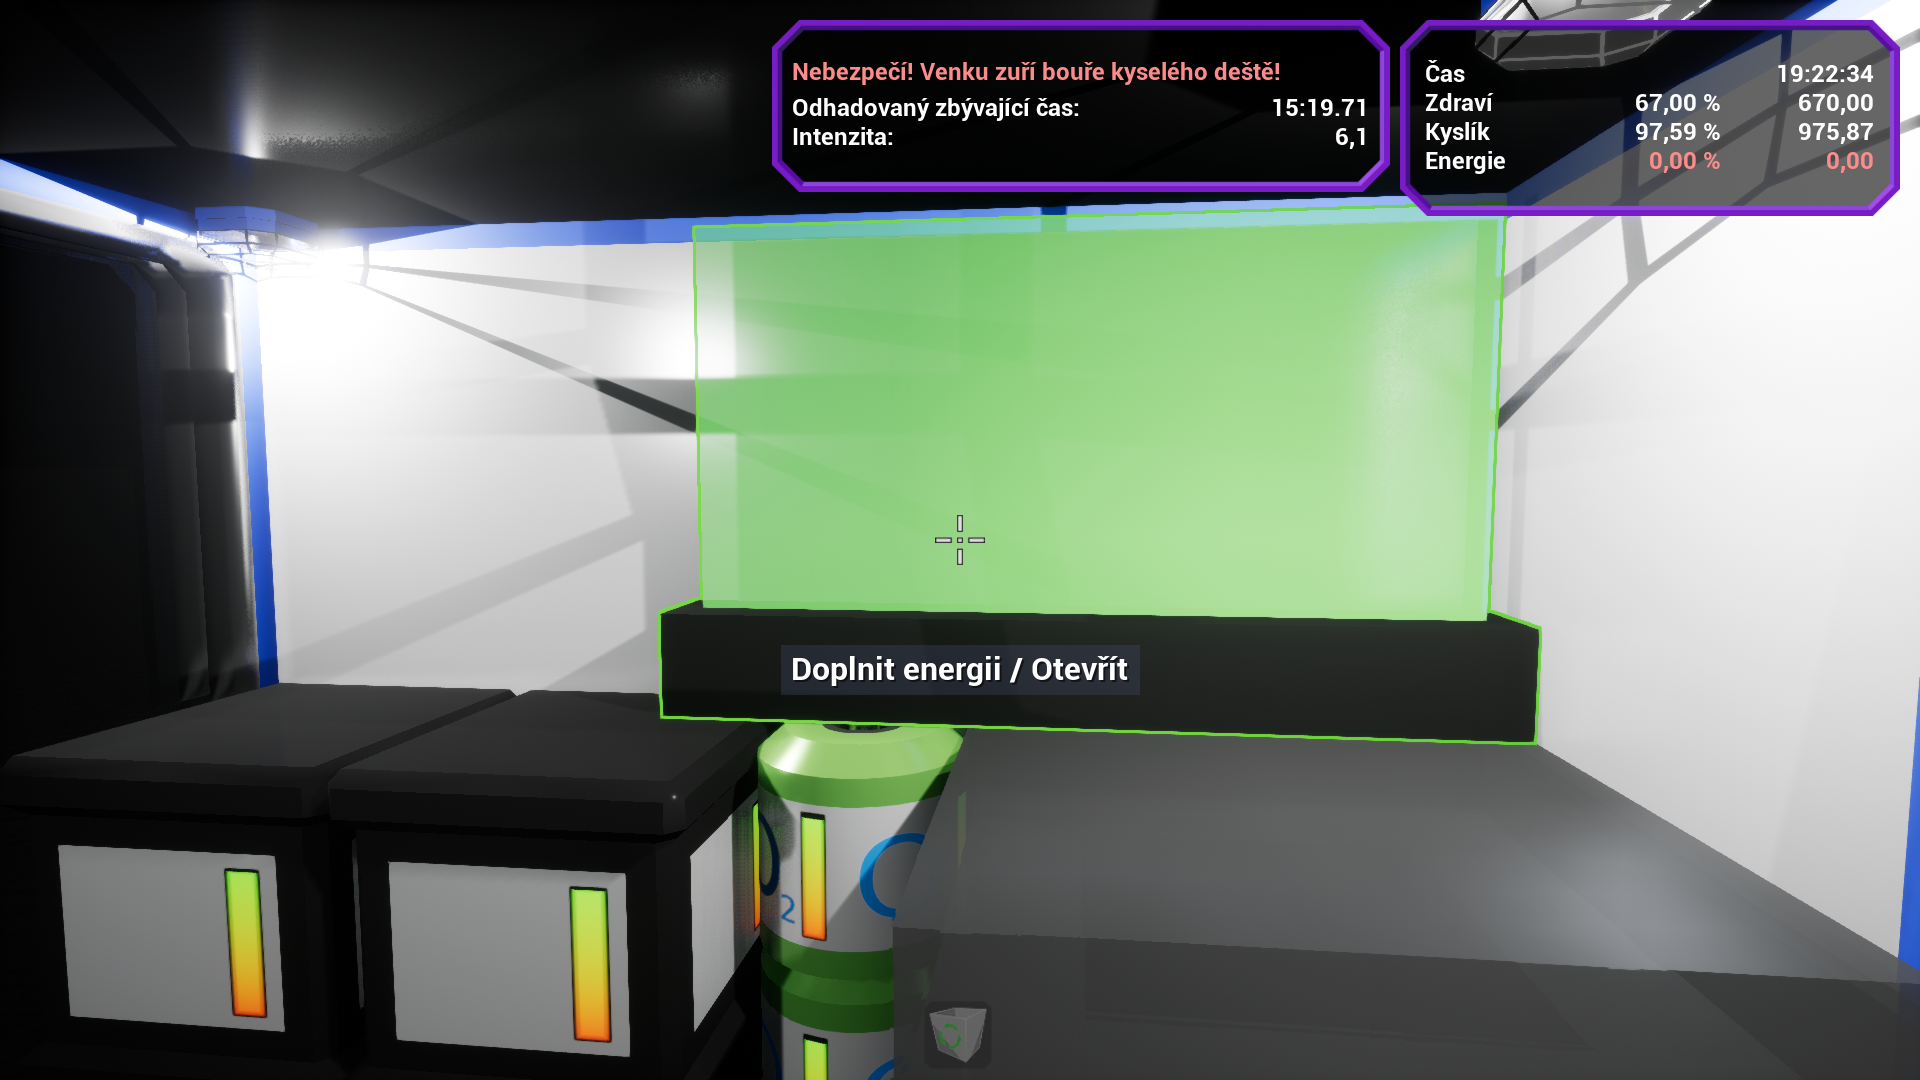
\includegraphics[ width=140mm]{../img/user/rain/2rainRefill}

\caption{Kyselý déšť - obnova zdraví}
\label{fig:user_rain_2rainRefill}

\end{figure}


\begin{figure}[!ht]\centering
\includegraphics[ width=140mm]{../img/user/rain/3rainRefill1}

\caption{Kyselý déšť - obnova zdraví}
\label{fig:user_rain_3rainRefill1}

\end{figure}

\FloatBarrier

Během bouře je též možné pozorovat animaci generátoru energie, kdy je po každém zásahu rozsvícen příslušný čtverec. Tuto animaci lze z menu vypnout a pokud má uživatel slabší stroj, tak to i doporučujeme.

\begin{figure}[!ht]\centering
\includegraphics[ width=140mm]{../img/user/rain/4rainGeneratorAnim}

\caption{Kyselý déšť - animace zásahů}
\label{fig:user_rain_4rainGeneratorAnim}

\end{figure}


\FloatBarrier




%!TEX root = ../prace.tex

\chapter{Závěr}


\section{Zhodnocení práce}


\section{Budoucí práce}


\begin{itemize}
	\item dynamičtějí mřížka? 20cm je nejspíše dost málo a vyžaduje to dost preciznosti // TODO zkusit pro test 25 či 30 cm a patřičným způsobem upravit velikosti modelů? (nejspíše to musí zůstat hardcoded, ale zkusím se nad tím zamyslet, pokud bude čas)
	\item vlastní sortování v seznamech

\end{itemize}

TODO dotazník?

%%% Seznam použité literatury
%%% Seznam použité literatury (bibliografie)
%%%
%%% Pro vytváření bibliografie používáme bibTeX. Ten zpracovává
%%% citace v textu (např. makro \cite{...}) a vyhledává k nim literaturu
%%% v souboru literatura.bib.
%%%
%%% Příkaz \bibliographystyle určuje, jakým stylem budou citovány odkazy
%%% v textu. V závorce je název zvoleného souboru .bst. Styly plainnat
%%% a unsrt jsou standardní součástí latexových distribucí. Styl czplainnat
%%% je dodáván s touto šablonou a bibTeX ho hledá v aktuálním adresáři.

\bibliographystyle{czplainnat}    %% Autor (rok) s českými spojkami
% \bibliographystyle{plainnat}    %% Autor (rok) s anglickými spojkami
% \bibliographystyle{unsrt}       %% [číslo]

\renewcommand{\bibname}{Seznam použité literatury}

%%% Vytvoření seznamu literatury. Pozor, pokud jste necitovali ani jednu
%%% položku, seznam se automaticky vynechá.

\bibliography{literatura}

%%% Kdybyste chtěli bibliografii vytvářet ručně (bez bibTeXu), lze to udělat
%%% následovně. V takovém případě se řiďte normou ISO 690 a zvyklostmi v oboru.

% \begin{thebibliography}{99}
%
% \bibitem{lamport94}
%   {\sc Lamport,} Leslie.
%   \emph{\LaTeX: A Document Preparation System}.
%   2. vydání.
%   Massachusetts: Addison Wesley, 1994.
%   ISBN 0-201-52983-1.
%
% \end{thebibliography}


%%% Obrázky v bakalářské práci
%%% (pokud jich je malé množství, obvykle není třeba seznam uvádět)
\listoffigures

%%% Tabulky v bakalářské práci (opět nemusí být nutné uvádět)
%%% U matematických prací může být lepší přemístit seznam tabulek na začátek práce.
%\listoftables

%%% Použité zkratky v bakalářské práci (opět nemusí být nutné uvádět)
%%% U matematických prací může být lepší přemístit seznam zkratek na začátek práce.

% Soubor se všemi zkratkami uvedenými v práci

%!TEX root = prace.tex


\chapter*{Seznam použitých zkratek}
\addcontentsline{toc}{chapter}{Seznam použitých zkratek}

TODO seznam zkratek

%%% Přílohy k bakalářské práci, existují-li. Každá příloha musí být alespoň jednou
%%% odkazována z vlastního textu práce. Přílohy se číslují.
%%%
%%% Do tištěné verze se spíše hodí přílohy, které lze číst a prohlížet (dodatečné
%%% tabulky a grafy, různé textové doplňky, ukázky výstupů z počítačových programů,
%%% apod.). Do elektronické verze se hodí přílohy, které budou spíše používány
%%% v elektronické podobě než čteny (zdrojové kódy programů, datové soubory,
%%% interaktivní grafy apod.). Elektronické přílohy se nahrávají do SISu a lze
%%% je také do práce vložit na CD/DVD. Povolené formáty souborů specifikuje
%%% opatření rektora č. 23/2016.
\chapwithtoc{Přílohy}

\openright
\end{document}
